%DIFAUXCMD\documentclass[acmsmall,screen,review,anonymous]{acmart}
%DIF LATEXDIFF DIFFERENCE FILE
%DIF DEL main-orig.tex   Fri Jul 10 02:26:04 2026
%DIF ADD main.tex        Tue Jul 21 00:40:28 2026
\usepackage{overpic}
\usepackage{xspace}
\usepackage{enumitem}
\usepackage{listings}
\usepackage{mathpartir}
\usepackage[dvipsnames]{xcolor}
\usepackage{stmaryrd}
%DIF 9a9-12
\usepackage{titlesec} %DIF >
 %DIF >
\newcommand{\lemref}[1]{\hyperref[#1]{Lemma~\ref*{#1}}} %DIF >
\newcommand{\defref}[1]{\hyperref[#1]{Definition~\ref*{#1}}} %DIF >
%DIF -------

% https://tex.stackexchange.com/questions/471464/inverted-exclamation-mark-in-mathmode
\DeclareMathSymbol{\mathinvertedexclamationmark}{\mathclose}{operators}{'074}
\DeclareMathSymbol{\mathexclamationmark}{\mathclose}{operators}{'041}

\makeatletter
\newcommand{\raisedmathinvertedexclamationmark}{%
  \mathclose{\mathpalette\raised@mathinvertedexclamationmark\relax}%
}
\newcommand{\raised@mathinvertedexclamationmark}[2]{%
  \raisebox{\depth}{$\m@th#1\mathinvertedexclamationmark$}%
}
\begingroup\lccode`~=`! \lowercase{\endgroup
  \def~}{\@ifnextchar`{\raisedmathinvertedexclamationmark\@gobble}{\mathexclamationmark}}
\mathcode`!="8000
\makeatother

\settopmatter{printacmref=false}

\newcommand{\coeff}{\,\raisebox{0.3ex}{\text{\scriptsize{@}}}\,}
\newcommand{\Timeline}{\textsc{Timeline}\xspace}
\renewcommand*{\sectionautorefname}{\S\!}
\renewcommand*{\subsectionautorefname}{\S\!}

\newcommand{\ident}[1]{\textsf{#1}}
\newcommand{\kvd}[1]{\textsf{\color{RoyalPurple}{#1}}}
\newcommand{\lsep}{\;\;|\;\;}
\newcommand{\cellref}[1]{\textsf{\color{Bittersweet}{#1}}}

%DIF 38a42-43
\newcommand{\caseref}[2]{\hyperref[#1]{Case~\#{}#2}} %DIF >
 %DIF >
%DIF -------
\newtheorem{theorem}{Theorem}
\newtheorem{lemma}[theorem]{Lemma}

\setcopyright{acmlicensed}
\copyrightyear{2026}
\acmYear{2026}
\acmDOI{XXXXXXX.XXXXXXX}

\acmJournal{JACM}
\acmVolume{37}
\acmNumber{4}
\acmArticle{111}
\acmMonth{8}

\DeclareRobustCommand*{\circled}[1]{\raisebox{-0.4ex}{\includegraphics[height=1.4\fontcharht\font`\B]{fig/circles/#1.pdf}}\hspace{0cm}}
\DeclareRobustCommand*{\circledsm}[1]{\includegraphics[height=1.1\fontcharht\font`\B]{fig/circles/#1.pdf}}

\lstdefinelanguage{lang}{
    morekeywords={false,and,not,if,then,else,let},
    morekeywords=[2]{pre,Behavior,Event,ggplot,aes,geom_point,geom_smooth,preserveAspectRatio,overlay,map,fillColor,column,image},
    morecomment=[l]{--},
    sensitive=true,
    morestring=[b]",
}
\lstdefinestyle{langStyle}{
    language=lang,
    basicstyle=\footnotesize\ttfamily,
    numbers=none,
    frame=none,
    stringstyle=\color{Sepia},
    showstringspaces=false,
    commentstyle=\color{gray},
    keywordstyle=\color{RoyalPurple},
    keywordstyle=[2]\color{Bittersweet},
    literate=
      {zz5}{{{\color{OliveGreen}{0.5}}}}3
      {syl}{{{\color{Bittersweet}{scale\_y\_log10}}}}{11}
      {1}{{{\color{OliveGreen}{1}}}}1
      {0}{{{\color{OliveGreen}{0}}}}1
      {~}{{\hspace{0.2em}}}1
  }


\lstdefinelanguage{timeline}{
    morekeywords={IF, AND, STEP, COS, RADIANS, MAX, SIN, POWER, SUM, POINT, GRAPH, STROKECOLOR,
      LINE, OVERLAY, AXES, KEYPRESS, IMAGE, FALSE, NOT, MIN,FILLCOLOR, COLUMN, APPEND, COORD,
%DIF 84c90
%DIF <       ASPECTRATIO, INDEX, INDIRECT, OFFSET, RANDOM, SQRT, RAND, DIST, NUMBER, DATASET, AVERAGE},
%DIF -------
      ASPECTRATIO, INDEX, INDIRECT, OFFSET, SQRT, RAND, DIST, NUMBER, DATASET, AVERAGE}, %DIF >
%DIF -------
    morekeywords=[2]{B5,C5,D5,E5,F5,B3,C3,D3,E3,F3,G3,H3,I3},
    sensitive=true,
    morestring=[b]",
    morecomment=[s]{/*}{*/}
}
\lstdefinestyle{timelineStyle}{
    language=timeline,
    commentstyle=\color{gray},
    basicstyle=\footnotesize\ttfamily,
    numbers=none,
    frame=none,
    showstringspaces=false,
    keywordstyle=\color{RoyalPurple},
    keywordstyle=[2]\color{Bittersweet},
    stringstyle=\color{Sepia},
    literate=
      {\$M16}{{{\color{Bittersweet}{\$M16}}}}3
      {\$N16}{{{\color{Bittersweet}{\$N16}}}}3
      {\$O16}{{{\color{Bittersweet}{\$O16}}}}3
      {\$G16}{{{\color{Bittersweet}{\$G16}}}}3
      {\$H16}{{{\color{Bittersweet}{\$H16}}}}3
      {\$I16}{{{\color{Bittersweet}{\$I16}}}}3
      {\$B\$6}{{{\color{Bittersweet}{\$B\$6}}}}4
      {\$D\$6}{{{\color{Bittersweet}{\$D\$6}}}}4
      {\$G\$6}{{{\color{Bittersweet}{\$G\$6}}}}4
      {\$C\$6}{{{\color{Bittersweet}{\$C\$6}}}}4
      {\$G\$10}{{{\color{Bittersweet}{\$G\$10}}}}5
      {\$B\$17}{{{\color{Bittersweet}{\$B\$17}}}}5
      {\$C\$17}{{{\color{Bittersweet}{\$C\$17}}}}5
      {\$O\$6}{{{\color{Bittersweet}{\$O\$6}}}}4
      {\$P\$6}{{{\color{Bittersweet}{\$P\$6}}}}4
      {\$Q\$6}{{{\color{Bittersweet}{\$Q\$6}}}}4
      {\$C\$10}{{{\color{Bittersweet}{\$C\$10}}}}5
      {\$D\$10}{{{\color{Bittersweet}{\$D\$10}}}}5
      {\$C11}{{{\color{Bittersweet}{\$C11}}}}4
      {\$D11}{{{\color{Bittersweet}{\$D11}}}}4
      {A1}{{{\color{Bittersweet}{A1}}}}2
      {B1}{{{\color{Bittersweet}{B1}}}}2
      {B5}{{{\color{Bittersweet}{B5}}}}2
      {B9}{{{\color{Bittersweet}{B9}}}}2
      {C9}{{{\color{Bittersweet}{C9}}}}2
      {D9}{{{\color{Bittersweet}{D9}}}}2
      {C1}{{{\color{Bittersweet}{C1}}}}2
      {C6}{{{\color{Bittersweet}{C6}}}}2
      {C8}{{{\color{Bittersweet}{C8}}}}2
      {E6}{{{\color{Bittersweet}{E6}}}}2
      {F6}{{{\color{Bittersweet}{F6}}}}2
      {E1}{{{\color{Bittersweet}{E1}}}}2
      {F1}{{{\color{Bittersweet}{F1}}}}2
      {D1}{{{\color{Bittersweet}{D1}}}}2
      {B10}{{{\color{Bittersweet}{B10}}}}3
      {C10}{{{\color{Bittersweet}{C10}}}}3
      {D10}{{{\color{Bittersweet}{D10}}}}3
      {E10}{{{\color{Bittersweet}{E10}}}}3
      {F10}{{{\color{Bittersweet}{F10}}}}3
      {G10}{{{\color{Bittersweet}{G10}}}}3
      {H10}{{{\color{Bittersweet}{H10}}}}3
      {I10}{{{\color{Bittersweet}{I10}}}}3
      {J10}{{{\color{Bittersweet}{J10}}}}3
      {K10}{{{\color{Bittersweet}{K10}}}}3
      {L10}{{{\color{Bittersweet}{L10}}}}3
      {U10}{{{\color{Bittersweet}{U10}}}}3
      {V10}{{{\color{Bittersweet}{V10}}}}3
      {O10}{{{\color{Bittersweet}{O10}}}}3
      {D14}{{{\color{Bittersweet}{D14}}}}3
      {P16}{{{\color{Bittersweet}{P16}}}}3
      {O16}{{{\color{Bittersweet}{O16}}}}3
      {C16}{{{\color{Bittersweet}{C16}}}}3
      {C35}{{{\color{Bittersweet}{C35}}}}3
      {C23}{{{\color{Bittersweet}{C23}}}}3
      {D17}{{{\color{Bittersweet}{D17}}}}3
      {D21}{{{\color{Bittersweet}{D21}}}}3
      {F19}{{{\color{Bittersweet}{F19}}}}3
      {E21}{{{\color{Bittersweet}{E21}}}}3
      {G19}{{{\color{Bittersweet}{G19}}}}3
      {D16}{{{\color{Bittersweet}{D16}}}}3
      {0}{{{\color{OliveGreen}{0}}}}1
      {-1}{{{\color{OliveGreen}{-1}}}}2
      {1}{{{\color{OliveGreen}{1}}}}1
      {2}{{{\color{OliveGreen}{2}}}}1
      {5}{{{\color{OliveGreen}{5}}}}1
      {cursor}{{{$\bullet$}}}1
      {~}{{\hspace{0.1em}}}1
}
\newcommand{\tml}[1]{\lstinline[style=timelineStyle,basicstyle=\small\ttfamily]{#1}}
\newcommand{\tmlsm}[1]{\lstinline[style=timelineStyle,basicstyle=\footnotesize\ttfamily]{#1}}
\newcommand{\lng}[1]{\lstinline[style=langStyle,basicstyle=\small\ttfamily]{#1}}
\newcommand{\todo}[1]{\textcolor{red}{\sffamily\small TODO: #1}}
%DIF PREAMBLE EXTENSION ADDED BY LATEXDIFF
%DIF UNDERLINE PREAMBLE %DIF PREAMBLE
\RequirePackage[normalem]{ulem} %DIF PREAMBLE
\RequirePackage{color}\definecolor{RED}{rgb}{1,0,0}\definecolor{BLUE}{rgb}{0,0,1} %DIF PREAMBLE
\providecommand{\DIFadd}[1]{{\protect\color{blue}\uwave{#1}}} %DIF PREAMBLE
\providecommand{\DIFdel}[1]{{\protect\color{red}\sout{#1}}}                      %DIF PREAMBLE
%DIF SAFE PREAMBLE %DIF PREAMBLE
\providecommand{\DIFaddbegin}{} %DIF PREAMBLE
\providecommand{\DIFaddend}{} %DIF PREAMBLE
\providecommand{\DIFdelbegin}{} %DIF PREAMBLE
\providecommand{\DIFdelend}{} %DIF PREAMBLE
\providecommand{\DIFmodbegin}{} %DIF PREAMBLE
\providecommand{\DIFmodend}{} %DIF PREAMBLE
%DIF FLOATSAFE PREAMBLE %DIF PREAMBLE
\providecommand{\DIFaddFL}[1]{\DIFadd{#1}} %DIF PREAMBLE
\providecommand{\DIFdelFL}[1]{\DIFdel{#1}} %DIF PREAMBLE
\providecommand{\DIFaddbeginFL}{} %DIF PREAMBLE
\providecommand{\DIFaddendFL}{} %DIF PREAMBLE
\providecommand{\DIFdelbeginFL}{} %DIF PREAMBLE
\providecommand{\DIFdelendFL}{} %DIF PREAMBLE
%DIF LISTINGS PREAMBLE %DIF PREAMBLE
\RequirePackage{listings} %DIF PREAMBLE
\RequirePackage{color} %DIF PREAMBLE
\lstdefinelanguage{DIFcode}{ %DIF PREAMBLE
%DIF DIFCODE_UNDERLINE %DIF PREAMBLE
  moredelim=[il][\color{red}\sout]{\%DIF\ <\ }, %DIF PREAMBLE
  moredelim=[il][\color{blue}\uwave]{\%DIF\ >\ } %DIF PREAMBLE
} %DIF PREAMBLE
\lstdefinestyle{DIFverbatimstyle}{ %DIF PREAMBLE
	language=DIFcode, %DIF PREAMBLE
	basicstyle=\ttfamily, %DIF PREAMBLE
	columns=fullflexible, %DIF PREAMBLE
	keepspaces=true %DIF PREAMBLE
} %DIF PREAMBLE
\lstnewenvironment{DIFverbatim}{\lstset{style=DIFverbatimstyle}}{} %DIF PREAMBLE
\lstnewenvironment{DIFverbatim*}{\lstset{style=DIFverbatimstyle,showspaces=true}}{} %DIF PREAMBLE
%DIF END PREAMBLE EXTENSION ADDED BY LATEXDIFF

\begin{document}
\title{Timeline: Adding the time dimension to spreadsheets}

\author{Authors}
\affiliation{%
  \institution{Place}
  \city{New York}
  \country{USA}}
\email{todo@todo}
\renewcommand{\shortauthors}{xx}

\begin{abstract}
Spreadsheets make it easy to express computations over two-dimensional data, but two dimensions
are not enough to express rich computations \DIFdelbegin \DIFdel{with }\DIFdelend \DIFaddbegin \DIFadd{involving }\DIFaddend time such as physics simulations, agent-based
\DIFdelbegin \DIFdel{models, analyses of financial data , or interactive systems.
}\DIFdelend \DIFaddbegin \DIFadd{modelling, financial data analyses, or simple interactive applications.
}

\DIFaddend We present \Timeline, a system that adds discrete time to spreadsheets. \DIFaddbegin \DIFadd{We motivate the design
of }\Timeline \DIFadd{through a small-scale formative study, present a }\emph{\DIFadd{core calculus}} \DIFadd{that
models system runtime, use it to formalise a static analysis to determine the required number of
past values, and evaluate the system using a series of case studies from the four aforementioned
areas.
}\DIFaddend

The \DIFdelbegin \DIFdel{remarkable insight from our work is }\DIFdelend \DIFaddbegin \DIFadd{paper also shows }\DIFaddend that a large number of advanced programming language concepts
can be directly applied in the context of spreadsheets with time. \Timeline draws from
\emph{dataflow languages} to express computations over time, \emph{coeffect systems} to ensure
bounded memory usage, \emph{functional reactive programming} to support interactivity, \DIFaddbegin \DIFadd{and
}\DIFaddend \emph{grammars of graphics} to support composable visualizations\DIFdelbegin \DIFdel{, and }\emph{\DIFdel{typed holes}} %DIFAUXCMD
\DIFdel{for
inserting cell references in the formula editor.
}%DIFDELCMD <

%DIFDELCMD < %%%
\DIFdel{In this paper, we provide an overview of the }%DIFDELCMD < \Timeline %%%
\DIFdel{design and discuss how it adapts the
aforementioned programming language innovations for the context of spreadsheets.
We formalize
the evaluation of spreadsheets with discrete time through a }\emph{\DIFdel{core calculus}}%DIFAUXCMD
\DIFdel{, describe a
coeffect-based static analysis that determines the required number of past values and prove that the
optimization is sound. More broadly, this paper shows that established programming language
ideas can often be productively used outside of their original domain.
}%DIFDELCMD <

%DIFDELCMD < %%%
\DIFdelend \DIFaddbegin \DIFadd{.
}\DIFaddend \end{abstract}

%%
%% The code below is generated by the tool at http://dl.acm.org/ccs.cfm.
%% Please copy and paste the code instead of the example below.
%%
\begin{CCSXML}
<ccs2012>
   <concept>
       <concept_id>10011007.10011006.10011008.10011009.10011022</concept_id>
       <concept_desc>Software and its engineering~Very high level languages</concept_desc>
       <concept_significance>500</concept_significance>
       </concept>
 </ccs2012>
\end{CCSXML}
\ccsdesc[500]{Software and its engineering~Very high level languages}
%%
%% Keywords. The author(s) should pick words that accurately describe
%% the work being presented. Separate the keywords with commas.
%\keywords{Spreadsheet systems, Dataflow languages, Functional programming}

% \received{20 February 2007}
% \received[revised]{12 March 2009}
% \received[accepted]{5 June 2009}

\begin{teaserfigure}
\begin{overpic}[width=\textwidth]{fig/flappy}
\put(10.2,45.5){\circledsm{A}}
\put(24.5,45.5){\circledsm{B}}
\put(38.5,45.5){\circledsm{C}}
%DIF < \put(38,42.4){\circledsm{D}}
\DIFdelbegin %DIFDELCMD < \put(18.5,9.5){\circledsm{1}}
%DIFDELCMD < \put(58,50.7){\circledsm{2}}
%DIFDELCMD < \put(10,2){\circledsm{3}}
%DIFDELCMD < \put(56.2,37){\circledsm{4}}
%DIFDELCMD < %%%
\DIFdelend \DIFaddbegin \put(18.5,9.5){\circledsm{4}}
\put(58,50.7){\circledsm{1}}
\put(10,2){\circledsm{2}}
\put(56.2,37){\circledsm{3}}
\DIFaddend \end{overpic}
\caption{A \DIFdelbegin \DIFdel{flappy bird }\DIFdelend \DIFaddbegin \DIFadd{Flappy Bird }\DIFaddend game clone in Timeline.
\circled{1} The \DIFdelbegin \DIFdel{selected formula computes the Y
velocity in }\DIFdelend \DIFaddbegin \DIFadd{system shows }\DIFaddend the current \DIFaddbegin \DIFadd{time }\DIFaddend step \DIFdelbegin \DIFdel{. }%DIFDELCMD < \circled{2} %%%
\DIFdel{The system uses discrete }\DIFdelend \DIFaddbegin \DIFadd{and lets the user advance step-by-step or
play/stop }\DIFaddend time.
\DIFdelbegin %DIFDELCMD < \circled{3} %%%
\DIFdelend \DIFaddbegin \circled{2} \DIFaddend Visualizations are built using a composable grammar \DIFdelbegin \DIFdel{of graphics }\DIFdelend and \DIFdelbegin %DIFDELCMD < \circled{4} %%%
\DIFdel{can be }\DIFdelend \DIFaddbegin \circled{3}
\DIFadd{are }\DIFaddend displayed \DIFdelbegin \DIFdel{inline or in a
separate panel}\DIFdelend \DIFaddbegin \DIFadd{on the side}\DIFaddend .
\DIFaddbegin \circled{4} \DIFaddend The \DIFaddbegin \DIFadd{selected }\DIFaddend formula \DIFdelbegin \DIFdel{for }\DIFdelend \DIFaddbegin \DIFadd{computes }\DIFaddend the \DIFaddbegin \DIFadd{Y }\DIFaddend velocity \DIFaddbegin \DIFadd{in the current step.
It }\DIFaddend \circled{A} specifies an initial value,
\circled{B} reacts to user-interface events, and \circled{C} \DIFdelbegin \DIFdel{accesses a previous value to compute
}\DIFdelend \DIFaddbegin \DIFadd{computes }\DIFaddend the current \DIFaddbegin \DIFadd{value using a previous }\DIFaddend one.}
\label{fig:teaser}
\vspace{0.5em}
\end{teaserfigure}

\maketitle

\section{Introduction}
Spreadsheets are sometimes referred to as ``the most widely used programming systems in the
world'' \cite{abraham-2009-prog}. Their uses range from personal productivity tools and
\DIFdelbegin \DIFdel{decision
making }\DIFdelend \DIFaddbegin \DIFadd{decision-making }\DIFaddend support systems to scientific analytical instruments and financial reporting
systems \cite{grossman-2023-taxonomy}. However, spreadsheets are \DIFdelbegin \DIFdel{first-order, limited to }\DIFdelend \DIFaddbegin \DIFadd{limited to flat }\DIFaddend tabular
data structures \DIFdelbegin \DIFdel{, }\DIFdelend and lack abstraction mechanisms.

Many extensions to the core spreadsheet model have been proposed, generalising the tabular
structure to non-tabular forms \cite{burnett-2001-forms3,bazant-2018-nontabular}, adding
support for objects \cite{mccutchen-2016-oop}, or incorporating support for streaming data
to use spreadsheets as the back-end for web development \cite{chang-2014-web,chang-2015-streaming}.
Abstraction mechanisms developed for spreadsheets include sheet-defined functions
\cite{jones-2003-functions,sestoft-2013-sheetdef} and gridlets \cite{joharizadeh-2020-gridlets},
while programming by example \cite{gulwani-2012-examples} simplifies data wrangling within
spreadsheets.

The above extensions show that extending spreadsheets is a difficult balancing act. How can we make
spreadsheets more expressive, while preserving their liveness, directness and
usability \cite{hermans-2016-spreadsheets}? The aim of \Timeline is to extend
spreadsheets with a built-in notion of discrete time, making it possible to use spreadsheets
in a range of domains that are difficult to tackle with only two dimensions \cite{litt-2017-multidim}
such as physics simulations, agent-based modelling \cite{abar-2017-abm}, financial data analysis,
or simple interactive applications. As illustrated in \autoref{fig:teaser}, \Timeline adds an
implicit discrete time to the spreadsheet programming model and extends the formula language to
allow references to previous values and user interface events, but otherwise preserves the
standard spreadsheet model.

\subsubsection*{Adapting programming language research.}
\DIFdelbegin \DIFdel{Although }\DIFdelend \Timeline is \DIFdelbegin \DIFdel{interesting as }\DIFdelend an exploration of the design, expressive power and usability of spreadsheets with
discrete time\DIFdelbegin \DIFdel{, this paper considers it primarily from the technical perspective
of
}\DIFdelend \DIFaddbegin \DIFadd{. We motivate the design through a small-scale formative study (}\autoref{sec:user-study}\DIFadd{)
and reflect on the trade-offs it introduces (}\autoref{sec:discussion}\DIFadd{). The technical core of
the paper presents }\Timeline \DIFadd{from the }\DIFaddend programming language design \DIFdelbegin \DIFdel{and implementation. The remarkable result is }\DIFdelend \DIFaddbegin \DIFadd{perspective. Notably,
we show }\DIFaddend that a large number of concepts and techniques developed in the context of programming
language research are directly applicable to spreadsheets \DIFaddbegin \DIFadd{with time}\DIFaddend .

\DIFdelbegin \DIFdel{The key addition to }\DIFdelend \Timeline \DIFdelbegin \DIFdel{is }\DIFdelend \DIFaddbegin \DIFadd{has }\DIFaddend a built-in notion of discrete time. Formulas \DIFdelbegin \DIFdel{in cells }\DIFdelend can refer to other
cells in the current time step (e.g.~\tml{G19}), but also values computed in earlier steps (e.g.~\tml{F19[-1]}).
The \DIFdelbegin \DIFdel{language design and runtime }\DIFdelend \DIFaddbegin \DIFadd{design and }\DIFaddend implementation of \Timeline \DIFdelbegin \DIFdel{draws }\DIFdelend \DIFaddbegin \DIFadd{draw }\DIFaddend inspiration from research on
\emph{synchronous dataflow languages} \cite{benveniste-2003-sync,halbwachs-1991-lustre}. To ensure
that simulations and interactive applications execute using bounded memory whenever possible,
we augment the runtime with a program analysis based on \emph{coeffects}
\cite{petricek-2013-coeffects,petricek-2014-coeffects}. The support for discrete \DIFdelbegin \DIFdel{times also }\DIFdelend \DIFaddbegin \DIFadd{time }\DIFaddend makes
it possible to use the spreadsheet paradigm for building interactive applications. Here, we draw
on the \emph{functional reactive programming} paradigm~\cite{elliott-1997-fran,wan-2000-frp}.
\DIFdelbegin \DIFdel{Although not strictly related to time}\DIFdelend \DIFaddbegin \DIFadd{To support visualizing time-varying values}\DIFaddend , \Timeline \DIFdelbegin \DIFdel{also }\DIFdelend adopts a \emph{composable data
visualization} model \cite{petricek-2021-compost,marasoiu-2019-cuscus,wilkinson-2012-gg}.
\DIFdelbegin \DIFdel{Finally, }%DIFDELCMD < \Timeline %%%
\DIFdel{also uses a notion of }\emph{\DIFdel{typed holes}} %DIFAUXCMD
\DIFdel{\mbox{%DIFAUXCMD
\cite{omar-2019-typedholes}
}\hspace{0pt}%DIFAUXCMD
to determine when the user may want to insert a cell reference during formula editing.
}\DIFdelend

\subsubsection*{Contributions\DIFaddbegin \DIFadd{.}\DIFaddend } This paper presents the design and implementation of \DIFaddbegin \Timeline\DIFadd{, }\DIFaddend a
spreadsheet system with discrete time\DIFaddbegin \DIFadd{, }\DIFaddend and captures its essence through a core calculus.

\DIFdelbegin %DIFDELCMD < \begin{itemize}[itemsep=2mm,topsep=2mm,leftmargin=0.5cm]
%DIFDELCMD < %%%
\DIFdelend \DIFaddbegin \begin{itemize}[itemsep=1.5mm,topsep=2mm,leftmargin=0.5cm]
\DIFaddend \item We provide an overview of the \Timeline design through a simple physics simulation
  \DIFdelbegin \DIFdel{example }\DIFdelend (\autoref{sec:walkthrough}) and examine the expressive power of the programming model
  through a number of case studies \DIFaddbegin \DIFadd{also }\DIFaddend covering agent-based modelling, \DIFdelbegin \DIFdel{physics simulations and finance
  }\DIFdelend \DIFaddbegin \DIFadd{financial data analysis,
  and interactive applications }\DIFaddend (\autoref{sec:case-studies}).

\item We discuss how the design and implementation of \Timeline adapts advanced
  programming language concepts for the context of spreadsheets
  (\autoref{sec:features}), including synchronous languages, coeffects,
  functional reactive programming, \DIFdelbegin \DIFdel{visualization grammars and typed holes}\DIFdelend \DIFaddbegin \DIFadd{and visualization grammars}\DIFaddend .

\item We present a core calculus of the \Timeline execution model (\autoref{sec:calculus}), which
  captures the way previous values are stored during the \DIFdelbegin \DIFdel{spreadsheet }\DIFdelend evaluation. We define a \DIFdelbegin \DIFdel{mechanism for checking }\DIFdelend \DIFaddbegin \DIFadd{static checking
  mechanism for }\DIFaddend references to earlier time steps\DIFdelbegin \DIFdel{(}%DIFDELCMD < \autoref{sec:calculus-timetypes}%%%
\DIFdel{)}\DIFdelend , formalize a space optimization \DIFdelbegin \DIFdel{based on coeffects (}%DIFDELCMD < \autoref{sec:calculus-optimization}%%%
\DIFdel{)
  and prove their soundness(}%DIFDELCMD < \autoref{sec:calculus-properties}%%%
\DIFdelend \DIFaddbegin \DIFadd{and prove its soundness.
}

\item \DIFadd{We motivate the }\Timeline \DIFadd{design through a small-scale formative study (}\autoref{sec:user-study}\DIFadd{)
  and discuss the resulting trade-offs using the cognitivie dimensions of notation framework (}\autoref{sec:discussion}\DIFaddend ).
\end{itemize}

\section{Overview}
\label{sec:walkthrough}

\DIFdelbegin \DIFdel{Although the focus of this paper is on the programming language aspects of }%DIFDELCMD < \Timeline%%%
\DIFdel{,
we first briefly review the design motivation for adding time to spreadsheets.
We then introduce }%DIFDELCMD < \Timeline %%%
\DIFdel{through an example that leverages the time dimension and
illustrates the capabilities of the system.
}%DIFDELCMD <

%DIFDELCMD < %%%
\subsubsection*{\DIFdel{Design Motivation}}
%DIFAUXCMD
\DIFdel{To motivate the design of }%DIFDELCMD < \Timeline%%%
\DIFdel{, we conducted formative interviews with spreadsheet experts,
including some with major applied experience \mbox{%DIFAUXCMD
\cite{govuk-2020-carbon}}\hspace{0pt}%DIFAUXCMD
, and we analysed models created using
modelling languages with discrete time \mbox{%DIFAUXCMD
\cite{ccl-2025-netlogo}}\hspace{0pt}%DIFAUXCMD
. The analysis shows that
tasks involving discrete time often require three dimensions. In agent-based
modeling \mbox{%DIFAUXCMD
\cite{abar-2017-abm}}\hspace{0pt}%DIFAUXCMD
, a simulation consists of multiple agents with multiple attributes
that evolve over time. Physics simulations that require numerical solution \mbox{%DIFAUXCMD
\cite{ccl-2025-netlogo}
}\hspace{0pt}%DIFAUXCMD
also require tracking multiple attributes of multiple entities over time. Financial analyses of
historical data have the same structure.
}%DIFDELCMD <

%DIFDELCMD < %%%
\DIFdel{Although conceptually simple, such modelling problems are difficult to represent in the traditional
spreadsheet paradigm. Using one dimension for time forces users to seek workarounds for encoding
the remaining two dimensions , for example by splitting attributes of individual agents across
separate tables. In practice, analysts are reluctant to use one of the two spreadsheet
dimensions for time. This has been confirmed by a formative interview participant,
who noted that }\emph{\DIFdel{``once you set the rows to time steps, you have
lost a dimension of your spreadsheet''}} %DIFAUXCMD
\DIFdel{and }\emph{\DIFdel{``if you use one }%DIFDELCMD < [%%%
\DIFdel{dimension}%DIFDELCMD < ] %%%
\DIFdel{for time,
everything else becomes miserable.''}} %DIFAUXCMD
%DIFDELCMD < \Timeline %%%
\DIFdel{aims to avoid such misery.
}%DIFDELCMD <

%DIFDELCMD < %%%
\subsubsection*{\DIFdel{Motivating Example}}
%DIFAUXCMD
\DIFdelend To demonstrate \Timeline, we consider a simple numerical \DIFdelbegin \DIFdel{physics }\DIFdelend simulation of cannonball firing.
In each step, the simulation computes the new cannonball position using the
position in the previous step and the current velocity. The initial velocity is computed from the
initial angle and firing speed and then updated using gravity and air drag, which itself depends
on the velocity in the previous step.
\DIFdelbegin \DIFdel{The simulation runs until the cannonballs hit the ground.
}\DIFdelend

There are three dimensions in the example: we have multiple cannonballs, with multiple attributes,
updated over multiple time steps. Implementing the simulation in a conventional spreadsheet is
possible, but challenging. \DIFdelbegin \DIFdel{One option is to have multiple tables, one for each attribute (X and
Y positions, X and Y velocities, X and Y air drags) with columns for individual cannonballs and
rows for time steps. This results in a complex structure with computation spread across 8 tables,
but it allows adding }\DIFdelend \DIFaddbegin \DIFadd{As discussed later (}\autoref{sec:discuss-grid}\DIFadd{), one option is having
a table for each of the attributes. This makes it possible to add }\DIFaddend cannonballs and time steps
using drag right and drag down operations (\DIFdelbegin \DIFdel{the
user selects the existing table and drags the selection }\DIFdelend to copy formulas to further empty cells)\DIFaddbegin \DIFadd{, but it results
in a complex structure with computation spread across 8 tables}\DIFaddend .


\begin{figure}
\begin{overpic}[width=\textwidth]{fig/cannon}
\put(80,34){\circledsm{1}}
\put(45,39.5){\circledsm{2}}
\put(33.5,19.4){\circledsm{3}}
\put(33.5,4.5){\circledsm{4}}
\put(95,20){\circledsm{5}}
\end{overpic}
\caption{Numerical cannonball firing simulation in \Timeline. \circled{1} Single table records attributes
of multiple cannonballs over time. \circled{2} The attributes are computed based on current and
previous values of other attributes. \circled{3} A separate table plots past positions as lines.
\circled{4} A table with configuration and composed final chart. \circled{5}~The composed chart
is then embedded in the sheet.}
\label{fig:cannon}
\vspace{-0.25em}
\end{figure}

\subsubsection*{Implementing Cannonball Simulation\DIFaddbegin \DIFadd{.}\DIFaddend }
In \Timeline, we can implement the cannonball simulation using a single table.
We use this example to introduce the key features of the system.

The calculation \DIFdelbegin \DIFdel{of the projectile motion is done in a single table that records }\DIFdelend \DIFaddbegin \DIFadd{keeps track of }\DIFaddend attributes of individual cannonballs over time
(\autoref{fig:cannon}, \circled{1}). The table includes the
current position (\tml{B3}, \tml{C3}), velocity (\tml{F3}, \tml{G3}) and air drag (\DIFdelbegin %DIFDELCMD < \tml{H3, I3}%%%
\DIFdelend \DIFaddbegin \tml{H3}\DIFadd{, }\tml{I3}\DIFaddend )
as well as the initial angle and speed (\tml{D3}, \tml{E3}). We discuss the calculation for the
first cannonball (row 3). Other cannonballs are added by selecting the last row and
using the drag down operation to copy its formulas, automatically updating the row references.

To specify the position of a cannonball, we need to give the initial position and then specify
how to compute the position in the current time step in terms of the value in the previous time step.
This illustrates two extensions that \Timeline makes to the core spreadsheet model. First, the
\tml{=>} operator specifies an initial value for a cell. Second, the notation \tml{C3[-1]} lets
us access the value of the cell \tml{C3} in a previous time step. For \DIFaddbegin \DIFadd{the }\DIFaddend cannonball, the initial
X and Y positions are 0, the position in later steps is computed by adding the current X and Y
velocities to the previous position and the computation stops if the cannonball hits the ground:

\begin{lstlisting}[style=timelineStyle]
/* Position X */ B3 = 0 => IF(C3[-1] < 0, B3[-1], B3[-1] + F3)
/* Position Y */ C3 = 0 => IF(C3[-1] < 0, C3[-1], C3[-1] + G3)
\end{lstlisting}

The calculation of the cannonball velocity again uses \tml{=>}. This time, the initial value is a
formula using the firing speed and angle (\tml{E3}, \tml{D3}). The velocity is then computed from
the value in the previous time step and air drag. For the Y velocity, we also subtract gravity,
which is a fixed cell reference (\tml{\$B\$17}) that is not updated during the drag down operation.
Air drag is obtained by multiplying the previous X and Y velocities by the air resistance (\tml{\$C\$17}):

\begin{lstlisting}[style=timelineStyle]
/* Velocity X */ F3 = E3 * COS(RADIANS(D3)) => F3[-1] + H3
/* Velocity Y */ G3 = E3 * SIN(RADIANS(D3)) => G3[-1] + I3 - $B$17
/* Air Drag X */ H3 = F3[-1] * $C$17
/* Air Drag Y */ I3 = G3[-1] * $C$17
\end{lstlisting}

Note that the calculation of air drag does not require specifying an initial value, because there are
no references to previous values of \tml{H3} and \tml{I3}. The \DIFdelbegin \DIFdel{only references to the cells are }\DIFdelend \DIFaddbegin \DIFadd{references }\DIFaddend in the
velocity computation \DIFdelbegin \DIFdel{, but those }\DIFdelend refer to the current value. The air drag computation accesses
velocity at the previous time step, which always exists because velocity defines an initial value
using \tml{=>}. \DIFaddbegin \DIFadd{At the first time step, }\tml{F3[-1]} \DIFadd{in the definition of the X air drag refers to
the initial velcotiy computed using trigonometric functions from the values of }\tml{E3} \DIFadd{and }\tml{D3}\DIFadd{.
}\DIFaddend As in standard spreadsheet systems, references between current values of cells
need to be acyclic. References to previous time steps do not introduce a cycle.

An interesting problem is how many past values need to be kept by the system. In the computation
described so far, we access one previous value of cells \tml{B3}, \tml{C3} and \tml{F3}, \tml{G3}
using the \tml{[-1]} notation. It is thus sufficient to keep one past value for these four cells.
For the chart (\autoref{fig:cannon}, \circled{5}) we need to store all previous values of the
cells that define the line. We discuss this aspect in detail in \autoref{sec:features-coeffects}.

\subsubsection*{Composable Data Visualization\DIFaddbegin \DIFadd{.}\DIFaddend }
Data visualizations in standard spreadsheet systems exist separately from the core spreadsheet
model. They are created through a graphical user interface where the user specifies data sources
and other chart attributes. \DIFaddbegin \DIFadd{With the additional time dimension, such user interface would grow
more complex, but visualizations in }\Timeline \DIFadd{also play a more central role. They
make it possible to see past values that are not directly displayed in the grid.
}\DIFaddend \Timeline takes inspiration from research on spreadsheet-based
and functional composable visualizations \cite{petricek-2021-compost,marasoiu-2019-cuscus}
and allows construction of visualizations directly in the spreadsheet.

The cannonball firing chart (\autoref{fig:cannon}, \circled{5}) is obtained by constructing
line charts that represent the movement of individual cannonballs over time and composing
the individual lines (\circled{3} and \circled{4}). This is done in a separate table that
contains one chart for each cannonball. \DIFdelbegin \DIFdel{Table }\DIFdelend \DIFaddbegin \DIFadd{The table }\DIFaddend row at index 10 (\tml{C10}, \tml{D10}) constructs
a line chart for cannonball at row index 3 (\tml{B3}, \tml{C3}):

\begin{lstlisting}[style=timelineStyle]
/* Point */ C10 = POINT(B3, C3)
/* Line */  D10 = GRAPH(STROKECOLOR(B10, LINE(C10[:-STEP()])))
/* Graph */ D17 = AXES("left bottom", OVERLAY(D10:D14))
\end{lstlisting}

The example uses a function \tml{POINT} that constructs a value representing a two-dimensional
point and a number of functions for constructing and transforming charts including
\tml{LINE}, \tml{OVERLAY} and \tml{AXES}. The latter are inspired by composable data visualizations
\cite{petricek-2021-compost}. \tml{LINE} takes a range of points and constructs a primitive chart
shape representing a line; \tml{OVERLAY} takes a range of chart shapes and constructs a single
chart shape consisting of the individual shapes; \tml{AXES} attaches axes with labels to a
given chart shape. \DIFdelbegin \DIFdel{The addition }\DIFdelend \DIFaddbegin \DIFadd{This }\DIFaddend requires adding points and chart shapes as two additional
primitive values to the core spreadsheet model. In systems that support richer data structures
\cite{mccutchen-2016-oop,yoder-1994-real,clack-1997-object,burnett-2001-forms3}, a point
could be a user-defined object or a record.

To construct the chart, the cell \tml{C10} constructs a point consisting of the current X and Y
positions of the cannonball. We then want to construct a line from all previous locations of the
cannonball. This is done by specifying a time range \tml{[:-STEP()]} in the cell reference.
The syntax is a shorthand for \tml{[-1:-STEP()]} and it selects all previous steps (\tml{STEP} is a
function that returns the number of the current step). The array of past values is then passed
to \tml{LINE}, which constructs a primitive chart shape. The \tml{GRAPH} function used in cell
\tml{D10} instructs \Timeline to display the chart inline in the cell as a sparkline \cite{frishberg-2011-sparklines}
without modifying the shape value. Finally, the cell \tml{D17} \DIFdelbegin \DIFdel{then }\DIFdelend overlays the
individual lines and adds axes. The underlying charting library automatically aligns the chart
elements and computes the range.

\subsubsection*{Extending the Spreadsheet Paradigm\DIFaddbegin \DIFadd{.}\DIFaddend }
The preceding example illustrated most of the extensions that \Timeline makes to the core
model of spreadsheets. In fact, the only significant additional feature needed by the
opening Flappy Bird clone (\autoref{fig:teaser}) is the \tml{KEYPRESS("A")} function, which
detects whether a key has been pressed \DIFaddbegin \DIFadd{in the current time step}\DIFaddend . The game movements and collision detection are
ordinary formulas and the game scene is constructed using the composable data visualization
library, leveraging the \tml{IMAGE} function to construct a primitive chart shape from an image URL.

The motivating example shows how the additions made in \Timeline preserve the simplicity
and directness of the core spreadsheet model. We add only a limited number of extensions
to the formula language (the \tml{=>} operator and references across time).
Moreover, when creating a spreadsheet in \Timeline, users still start with concrete values and then
extend their formulas using the drag down operation to apply a formula across a range of inputs,
preserving the \emph{from concrete cases} mode of \emph{abstraction construction} \cite{jakubovic-2023-techdims}.

\section{Research themes}
\label{sec:features}

Syntactically, the only extensions that \Timeline makes to the core spreadsheet model are the
operator for specifying the \DIFdelbegin \DIFdel{previous (default) }\DIFdelend \DIFaddbegin \DIFadd{initial }\DIFaddend value \tml{=>} and a notation for accessing
previous values \tml{A1[-1]} or time ranges \DIFdelbegin %DIFDELCMD < \tml{A1[-1:STEP()]}%%%
\DIFdelend \DIFaddbegin \tml{A1[-1:-STEP()]}\DIFaddend . However, the design and
implementation of \Timeline \DIFdelbegin \DIFdel{draws }\DIFdelend \DIFaddbegin \DIFadd{draw }\DIFaddend on a number of research directions on programming languages
that have previously not been connected to spreadsheets. This section provides an overview
discussing the major connections. More formal treatment
(\autoref{sec:calculus}) and case studies (\autoref{sec:case-studies}) follow in later sections.

\subsection{Synchronous languages}
\label{sec:features-dataflow}

The notion of discrete time, as implemented in \Timeline, is based on the notion of time
in declarative synchronous programming languages. Synchronous languages \cite{benveniste-2003-sync}
are based on the idea that time proceeds in discrete logical ticks and components react
concurrently to changes in each step. The approach has been successful in areas such
as signal processing and embedded control systems.

In imperative synchronous languages such as Esterel \cite{berry-1992-esterel}, programs explicitly
await and emit time signals. Our approach is akin to declarative synchronous languages like
Lucid and Lustre \cite{ashcroft-1977-lucid,caspi-1987-lustre} where expressions denote streams
of values and operators and functions operate on streams in a pointwise manner. The languages
additionally include a number of operators for manipulating streams. Consider the following
Lustre example adapted from \cite{benveniste-2003-sync}:

\begin{lstlisting}[style=langStyle]
      nat = 0 -> pre(nat) + 1;
     edge = false -> (c and not pre(c));
edgecount = if edge then pre(edgecount) + 1 else pre(edgecount)
\end{lstlisting}

The definition of \lng{nat} illustrates two operators for manipulating streams.
The \lng{e1 -> e2} operator creates a stream that has the value of the stream \lng{e1} in the
first time step and the value of \lng{e2} in subsequent steps. The \lng{pre(e)} operator
constructs a stream that, in a time step $t$, returns the value of \lng{e} in \DIFdelbegin \DIFdel{a }\DIFdelend time step $t\!-\!1$.
The \DIFdelbegin \DIFdel{examples can be directly implemented in }\DIFdelend \DIFaddbegin \DIFadd{Lustre examples map directly to }\DIFaddend \Timeline:

\begin{lstlisting}[style=timelineStyle]
      /* nat */ A1 = 0 => A1[-1] + 1
     /* edge */ C1 = FALSE => AND(B1, NOT(B1[-1]))
/* edgecount */ D1 = IF(C1, D1[-1] + 1, D1[-1])
\end{lstlisting}

\DIFdelbegin \DIFdel{The Lustre examples map directly to }%DIFDELCMD < \Timeline%%%
\DIFdel{. }\DIFdelend Although we do not explain, or formally model,
\Timeline in terms of streams, in practice our \tml{=>} and \tml{[-1]} operations provide the same
functionality as \lng{->} and \lng{pre} in Lustre. Of course, Lustre also provides higher-order
abstraction capabilities that are not present in \Timeline, but those could be supported through
some of the proposed abstraction mechanisms for spreadsheets
\cite{sestoft-2013-sheetdef,jones-2003-functions,mccutchen-2020-sdfs}.

It is also worth noting that these examples could
\DIFdelbegin \DIFdel{also }\DIFdelend be easily encoded in an ordinary two-dimensional spreadsheet (using rows for time steps).
As illustrated by our case study from the finance domain (\autoref{sec:case-finance}) \DIFdelbegin \DIFdel{the above
way of }\DIFdelend encoding
stream processing in \Timeline \DIFaddbegin \DIFadd{using built-in time }\DIFaddend is practically useful when working with
large data sets.

\subsection{Coeffect analysis}
\label{sec:features-coeffects}

An interesting problem that \Timeline shares with synchronous languages is how many past values
need to be stored and whether the buffer size is bounded \cite{caspi-1992-clocks,caspi-2008-lucid}.
In all the examples in \autoref{sec:features-dataflow}, the memory is bounded---the runtime needs to store one past
value for each cell accessed via \tml{[-1]}.

\DIFdelbegin %DIFDELCMD < \begin{figure}[b]
%DIFDELCMD < %%%
\DIFdelendFL \DIFaddbeginFL \begin{figure}[t]
\DIFaddendFL \vspace{-1em}
\[
\inferrule
  {x\!:\!\tau\in\Gamma}
  {\Gamma \coeff 0 \vdash x : \tau}
\qquad
\inferrule
  {\Gamma \coeff n \vdash e : \tau}
  {\Gamma \coeff n\!+\!1 \vdash \mathsf{prev}~e : \tau}
\qquad
\inferrule
  {\Gamma \coeff m \vdash e_1 : \tau_1 \DIFdelbeginFL \DIFdelFL{\xrightarrow{t} }\DIFdelendFL \DIFaddbeginFL \DIFaddFL{\xrightarrow{k} }\DIFaddendFL \tau_2 \quad
    \Gamma \coeff n \vdash e_2 : \tau_1}
  {\Gamma \coeff \mathsf{max}(m,n+\DIFdelbeginFL \DIFdelFL{t}\DIFdelendFL \DIFaddbeginFL \DIFaddFL{k}\DIFaddendFL ) \vdash e_1~e_2 : \tau_2}
\]
\vspace{-0.5em}
\caption{Coeffect typing rules for variables, previous value access and application.}
\label{fig:coeffects-calculus}
\vspace{-0.5em}
\end{figure}

In \Timeline, we adopt a static analysis based on dataflow coeffects
\cite{petricek-2013-coeffects,brunel-2014-coeffects,petricek-2014-coeffects}. A type system
based on coeffects annotates expressions with context requirements, such as variable liveness
or, in the case of dataflow, the number of required past values. In dataflow coeffects,
type judgements of the form $\Gamma \coeff n \vdash e : \tau$ indicate that a given expression $e$
can be evaluated in a variable context $\Gamma$ with at least $n$ past values for
each of the variables. Structural coeffects \cite{petricek-2014-coeffects} are more precise
and track context requirements per-variable, by using a vector of annotations and explicit
weakening, contraction and exchange rules. \autoref{fig:coeffects-calculus} shows three of the
coeffect typing rules.

The rule for variables states that accessing the current value of a variable does not require
any past values. This is akin to a cell reference such as \tml{B1}. The rule for $\kvd{prev}~e$
indicates that, if evaluating $e$ requires $n$ past values, then obtaining the previous value
of $e$ requires $n+1$ past values. Function types in the coeffect calculus are annotated
with how many past values the function requires (a function $\lambda x.\kvd{prev}~x$ would be
annotated with $1$). The rule for function application thus combines context requirements of the
expression that defines the function with the context requirements of the evaluation of the
argument, followed by the evaluation of the function (if evaluating the argument requires
$n$ past values and the function needs \DIFdelbegin \DIFdel{further $t$ }\DIFdelend \DIFaddbegin \DIFadd{$k$ additional }\DIFaddend past values, then evaluating the function call
requires \DIFdelbegin \DIFdel{$n+t$ }\DIFdelend \DIFaddbegin \DIFadd{$n+k$ }\DIFaddend past values).

In \Timeline, we can only access previous values via a cell reference. Computations such as
$\kvd{prev}(a+b)$ can be expressed by storing $a+b$ in a cell, say \tml{A1}, and accessing \tml{A1[-1]}.
Time ranges in \Timeline can be dynamic, e.g., \tml{C10[:-STEP()]}, or even indirect,
e.g., \tml{A1[-B1]}. Such references cannot be statically checked and so the inferred number
of required past values can be unbounded.

We describe the type system for checking previous value references formally in
\autoref{sec:calculus-timetypes}. The type system is used in two ways. First, it is used to
determine the size of buffers required to store past values during spreadsheet execution.
Second, it is used to check that a sufficient number of previous values is specified using the
\tml{=>} operator (for cells with potentially unbounded number of past values, we assume that the
first use of \tml{=>} specifies a default value for any previous time step; an alternative design
would be to have a separate operator for this purpose).

A basic static checking mechanism simply ensures that a cell referenced via \tml{A1[-n]} has
at least $n$ past values, but the coeffect calculus suggests a more flexible semantics.
\DIFdelbegin \DIFdel{Consider for example }\DIFdelend \DIFaddbegin \DIFadd{The following example shows how the same computation admits two evaluation strategies with different
memory use}\DIFaddend :

\begin{lstlisting}[style=timelineStyle]
            /* counter */ A1 = 0 => A1[-1] + 1
      /* prev(counter) */ B1 = 0 => A1[-1]
/* prev(prev(counter)) */ C1 = B1[-1]
\end{lstlisting}

We refer to cells that require storing past values as \emph{stateful} and cells that are
always computed instantaneously as \emph{stateless}. Note that the same distinction is made
in synchronous languages, where expressions may be stateless/combinatorial/memoryless or
stateful/with memory.

In the above example, \tml{A1} and \tml{B1} are stateful and require 1 past value each.
Correspondingly, we specify one previous value for each of the cells using \tml{=>}.
However, the same spreadsheet could be executed by making \tml{B1} stateless and requiring
two past values of \tml{A1}:

\begin{lstlisting}[style=timelineStyle]
            /* counter */ A1 = 0 => 1 => A1[-1] + 1
      /* prev(counter) */ B1 = A1[-1]
/* prev(prev(counter)) */ C1 = B1[-1]
\end{lstlisting}

This alternative corresponds to the application rule of the coeffect calculus where the context
requirements of a function argument and the context requirements of a function are combined.
If we make \tml{B1} stateless, we can always recompute its single previous value using the second
past value of \tml{A1}. We discuss this coeffect-based generalisation of past value access checking
in \autoref{sec:calculus-optimization}.

\DIFdelbegin \DIFdel{In practice, static analysis that ensures }\DIFdelend \DIFaddbegin \DIFadd{Ensuring }\DIFaddend bounded buffer sizes for stateful cells in \Timeline
\DIFdelbegin \DIFdel{is crucial }\DIFdelend \DIFaddbegin \DIFadd{matters }\DIFaddend for an efficient execution of all of the \Timeline applications (\autoref{sec:case-studies})\DIFdelbegin \DIFdel{.
}\DIFdelend \DIFaddbegin \DIFadd{,
}\DIFaddend Unbounded buffers are only needed in situations such as the cannonball visualization
(\autoref{sec:walkthrough}) where we explicitly access all past data to draw a chart, but
the \DIFdelbegin \DIFdel{flappy bird clone }\DIFdelend \DIFaddbegin \DIFadd{Flappy Bird }\DIFaddend game (\autoref{fig:teaser}) requires only one past value of several cells,
rather than storing all previously encountered states. \DIFdelbegin \DIFdel{Optionally, }\DIFdelend \DIFaddbegin \DIFadd{In practice, our case studies are small
enough that memory is not a practical constraint and }\DIFaddend \Timeline makes it possible to keep
all past values \DIFdelbegin \DIFdel{, which enables }\DIFdelend \DIFaddbegin \DIFadd{to enable }\DIFaddend stepping back through time for debugging.

The generalised coeffect-based execution makes it possible to trade space for time. This is
theoretically interesting and it is useful in cases where, for example, a large table
has a column of values that all depend on a single cell outside of the table. The optimization may
reduce the memory footprint, although this would be practically useful only in limited execution
environments.

\subsection{Functional reactive programming}
\label{sec:features-frp}

Functional reactive programming (FRP) \cite{elliott-1997-fran,wan-2000-frp} is a programming
paradigm for building reactive and interactive applications in functional programming languages.
Given the close connection between spreadsheets and functional programming \cite{burnett-2001-forms3},
it is not surprising that \Timeline can draw \DIFdelbegin \DIFdel{ideas from }\DIFdelend \DIFaddbegin \DIFadd{on }\DIFaddend functional reactive programming \DIFaddbegin \DIFadd{ideas}\DIFaddend .

In FRP, programs are structured in terms of two abstractions: \emph{behaviors} model time-varying
values and \emph{events} represent discrete event occurrences. Programs are constructed using a
number of combinators that relate the two abstractions. In Fran~\cite{elliott-1997-fran}
the type \lng{Behavior~a} represents streams of values of type \lng{a}, while \lng{Event~a}
represents discrete events emitting values of type \lng{a}. The two abstractions are composed
using combinators such as \lng{untilB}:

\begin{lstlisting}[style=langStyle]
-- Behave as the initial behavior, changing to the one emitted by the event
untilB :: Behavior a -> Event (Behavior a) -> Behavior a
\end{lstlisting}

The behavior \lng{untilB start evt} has the value of \lng{start} initially. When \lng{evt}
occurs, the value becomes that of the time-varying value emitted by the event. In
Yampa \cite{courtney-2003-yampa,hudak-2003-arrows}, behaviors are represented using arrows
\lng{SF a b} from input \lng{a} to output \lng{b}, which can be composed using a family of
switch combinators such as:

\begin{lstlisting}[style=langStyle]
-- Switch to a new signal function 'SF a b' whenever the specified event occurs
switch :: SF a (b, Event c) -> (c -> SF a b) -> SF a b
\end{lstlisting}

Conceptually, FRP systems are based on a continuous notion of time. Together with the rich
higher-order primitives, this has historically been difficult to implement efficiently
\cite{krishnaswami-2013-leaks,bahr-2022-frp} and some implementations adopted a model with
clocks \cite{wan-2002-efrp} more akin to synchronous languages. \Timeline is based on
discrete time and so it eschews such implementation difficulties.
\DIFdelbegin \DIFdel{However}\DIFdelend \DIFaddbegin

\Timeline \DIFadd{also does not use switching functions to dynamically reconfigure the dataflow graph
as in some FRP systems \mbox{%DIFAUXCMD
\cite{cooper-2006-frtime}}\hspace{0pt}%DIFAUXCMD
. When the projectile hits the ground in the
cannonball simulation, the simulation continues running but the value is no longer updated.
(The }\Timeline \DIFadd{user interface allows specifying a reset condition outside of the formula language,
which is used in the Flappy Bird clone.) Despite these limitations}\DIFaddend , it is still \DIFdelbegin \DIFdel{possible }\DIFdelend \DIFaddbegin \DIFadd{useful }\DIFaddend to
view \Timeline formulas as specifying time-varying behaviors.
\DIFdelbegin \DIFdel{The }%DIFDELCMD < \tml{=>} %%%
\DIFdel{operator is akin to }%DIFDELCMD < \lng{untilB} %%%
\DIFdel{and constructs a behavior that changes when the
clock tick event occurs.
}\DIFdelend

Our main inspiration from functional reactive programming is for the integration of events
into the programming model of \Timeline. For example, in the \DIFdelbegin \DIFdel{flappy bird }\DIFdelend \DIFaddbegin \DIFadd{Flappy Bird }\DIFaddend clone
(\autoref{fig:teaser}), the key press event controls the velocity of the bird.
In the game, the cells \tml{\$O\$6}, \tml{\$P\$6}, and \tml{\$Q\$6} contain constants that
specify the gravity, jump speed and maximal velocity. The new velocity is\DIFdelbegin \DIFdel{computed as}\DIFdelend :

\begin{lstlisting}[style=timelineStyle]
/* Velocity */ D21 = 0 => MIN($Q$6, IF(KEYPRESS("A"), -$P$6, D21[-1] + $O$6))
\end{lstlisting}

In \Timeline, we can think of \DIFdelbegin %DIFDELCMD < \tml{IF(KEYPRESS("A"), .., ..))} %%%
\DIFdelend \DIFaddbegin \tml{IF(KEYPRESS("A"), .., ..)} \DIFaddend as a switching operator akin to
\lng{untilB} or \lng{switch} that changes the behavior from one time-varying value to another
when the event occurs. However, because of the discrete time model, the behavior changes once
and the state is stored implicitly in the history of the cell, rather than explicitly using
accumulator combinators as in FRP.

\subsection{Composable data visualizations}
\label{sec:features-datavis}

In traditional spreadsheets, visualizations are created outside of the formula language and
data is selected through a user interface. \DIFdelbegin \DIFdel{This approach is not reproducible,
does not enable
learning \mbox{%DIFAUXCMD
\cite{sarkar-2018-learn} }\hspace{0pt}%DIFAUXCMD
and is difficult to extend to data sources with the time
dimension or richer visualizations }\DIFdelend \DIFaddbegin \DIFadd{As noted earlier (}\autoref{sec:walkthrough}\DIFadd{),
}\Timeline \DIFadd{provides a more flexible, formula-based mechanism that makes it easy to display not just
the current but also past values that are not directly visible in the grid. It makes it possible
to build rich visualizations across multiple dimensions, and it also enables users to learn how
to construct visualizations by examining existing spreadsheets \mbox{%DIFAUXCMD
\cite{sarkar-2018-learn}}\hspace{0pt}%DIFAUXCMD
}\DIFaddend .

Research that originates from grammar of graphics \cite{wilkinson-2012-gg} offers a more
declarative and compositional alternative \cite{satyanarayan-2017-vegalite,wickham-2010-layered}.
In systems based on the grammar of graphics, a chart is created by putting together
data, scales that transform data to visual values, coordinate system, geometric marks that
specify how to display data, data transformations and other aspects of visualization.
For example, using the ggplot2 library \cite{wickham-2010-layered} we can compose a chart as:

\begin{lstlisting}[style=langStyle]
ggplot(diamonds, aes(x = carat, y = price)) +
  geom_point(alpha = zz5) + geom_smooth() + syl()
\end{lstlisting}

The snippet separately specifies the data source \ident{diamonds}, aesthetics that \DIFdelbegin \DIFdel{maps }\DIFdelend \DIFaddbegin \DIFadd{map }\DIFaddend properties
\ident{carat} and \ident{price} from the data source to X and Y coordinates, adds two geometric
marks (points and smooth line) and makes the Y scale logarithmic. Grammar of graphics is very
effective for scientific visualizations, but it assumes \DIFaddbegin \DIFadd{a }\DIFaddend two-dimensional data source, requires a
large number of primitive constructs and its range of charts is still limited.

\begin{figure}
\begin{overpic}[width=\textwidth]{fig/fruits}
\put(41,15.3){\circledsm{1}}
\put(50.5,15.3){\circledsm{2}}
\put(21.2,2.5){\circledsm{3}}
\put(95,15.5){\circledsm{4}}
\end{overpic}
\caption{Composing rich data visualization in \Timeline. \circled{1} Columns are constructed
using the fruit name and popularity. \circled{2} Image for each fruit is loaded, positioned and
also displayed inside the table. \circled{3} Columns and images are composed in a single cell,
\circled{4} which is displayed as a chart in the spreadsheet.}
\label{fig:fruits}
\DIFdelbeginFL %DIFDELCMD < \vspace{-0.25em}
%DIFDELCMD < %%%
\DIFdelendFL \end{figure}

\DIFdelbegin \DIFdel{~
}%DIFDELCMD <

%DIFDELCMD < %%%
\DIFdelend A more flexible approach, which fits well with the spreadsheet paradigm\DIFaddbegin \DIFadd{, }\DIFaddend is based on the
composition of graphical shapes. This has been developed in the context of functional
programming \cite{petricek-2021-compost}, but is conceptually similar to a design prototype
envisioned for spreadsheets \cite{marasoiu-2019-cuscus}.

In composable visualizations, graphical shapes are specified using domain values such
as exchange rate, number of votes, country names, or population. When composed, the
system infers composite scales, checks that all shapes have a compatible scale, and arranges
individual shapes. This makes it possible to compose visualizations that combine different
visual elements generated from data. For example, the following
uses Compost.js \cite{petricek-2017-compostjs} to overlay fruit images over a column chart:

\begin{lstlisting}[style=langStyle]
let fruitBars =
  c.preserveAspectRatio("none", c.overlay(fruits.map(f =>
    c.overlay([
      c.fillColor(f.color,
        c.column(f.kind, f.value)),
      c.image("img/" + f.kind + ".png",
        [[f.kind, 0], 0], [[f.kind, 1], f.value]) ])
    )))
\end{lstlisting}

The snippet iterates over the data using \lng{fruits.map}. For each data point, it
creates a column and an image and overlays the two. The X scale is categorical and
the image position is specified as \lng{[f.kind,0]} and \lng{[f.kind,1]}, which defines
the left and the right end of the area allocated for the category \lng{f.kind}. The Y scale is
continuous and the values are numbers. The individual images are combined using
\lng{overlay} and the snippet uses \lng{preserveAspectRatio} to enable scaling.

As shown in \autoref{fig:fruits}, the same chart can be constructed in \Timeline.
We specify input data in a table and add two columns representing the column and
image. Those are then overlaid in cell \tml{C8}:

\begin{lstlisting}[style=timelineStyle]
/* Construct column and image graphical shapes for each data point */
E3 = FILLCOLOR(COLUMN(B3, C3))
F3 = GRAPH(IMAGE(APPEND(B3, ".png"), POINT(COORD(B3,0),0), POINT(COORD(B3,1), 1)))
\end{lstlisting}

\vspace{-0.25em}
\begin{lstlisting}[style=timelineStyle]
/* Overlay chart elements and specify additional chart properties */
C8 = AXES("left bottom", ASPECTRATIO("none", OVERLAY(E3:E6,F3:F6)))
\end{lstlisting}

The column is constructed using \tml{COLUMN} which takes a categorical value (fruit name)
and a numerical value (fruit popularity). It creates a rectangle that spans the whole area allocated
for the category in the X dimension and ranges from 0 to the specified value in the Y dimension.
When loading an image, we construct the image URL (simplified for presentation) and specify its
location using \tml{COORD}, which creates a categorical coordinate and \tml{POINT}, which combines
X and Y coordinates. Note that \tml{COLUMN} is built on top of a primitive for filling \DIFaddbegin \DIFadd{a }\DIFaddend polygon
that takes a list of points.

The programming model offered by composable visualizations in \Timeline offers many of the user
experiences prototyped in Cuscus \cite{marasoiu-2019-cuscus}. \DIFdelbegin \DIFdel{Like }\DIFdelend \DIFaddbegin \DIFadd{As }\DIFaddend in Cuscus, the graphical shape of a
visualization can be specified using formulas in a table that supports the drag down operation,
enabling non-programmers to create visualizations using tools they are already familiar with.
\Timeline improves on Cuscus in that it specifies shape dimensions in domain values and allows
more flexible composition, such as overlaying a specified range. Visual shapes in \Timeline cannot
be, however, modified using direct manipulation. The encouraging results of user studies performed
for Cuscus thus likely also apply to visualizations in \Timeline.

\begin{figure}
\DIFdelbeginFL %DIFDELCMD <

%DIFDELCMD < %%%
\DIFdelFL{\raisebox{-0.45\height}{\begin{overpic}[width=10em]{fig/holes1}\put(88,53){\circledsm{1}}\end{overpic}}
$~~\boldsymbol{\Rightarrow}~~$
\raisebox{-0.45\height}{\begin{overpic}[width=10em]{fig/holes2}\put(88,53){\circledsm{2}}\end{overpic}}
$~~\boldsymbol{\Rightarrow}~~$
\raisebox{-0.45\height}{\begin{overpic}[width=10em]{fig/holes3}\put(88,53){\circledsm{3}}\end{overpic}}
}%DIFDELCMD < \caption{%
{%DIFAUXCMD
\DIFdelFL{Constructing a formula for Fahrenheit to Celsius conversion. }%DIFDELCMD < \circled{1}
%DIFDELCMD < %%%
\DIFdelFL{After typing "(" the user clicks on a wrong cell and a reference to it is inserted,
}%DIFDELCMD < \circled{2} %%%
\DIFdelFL{then they click on the right cell to correct the formula. }%DIFDELCMD < \circled{3} %%%
\DIFdelFL{After
writing the rest of the formula, they click anywhere on the sheet to stop editing it.}}
%DIFAUXCMD
%DIFDELCMD < \label{fig:holes}
%DIFDELCMD < \end{figure}
%DIFDELCMD <

%DIFDELCMD < \newcommand{\hhole}[1]{{\color{Purple}{\llparenthesis}} \hspace{0.05em} #1 \hspace{0.05em} {\color{Purple}{\rrparenthesis}}}
%DIFDELCMD < \newcommand{\errrec}[1]{{\color{Emerald} #1}}
%DIFDELCMD < \newcommand{\hcmt}[1]{\text{\color{gray}\small #1}}
%DIFDELCMD <

%DIFDELCMD < \begin{figure}[t]
%DIFDELCMD < \vspace{-0.5em}
%DIFDELCMD < %%%
\[
\DIFdelFL{\begin{array}{r@{\;\;}r@{\;\;}l}
\hhole{}
 & \rightsquigarrow & (\hhole{}\errrec{)} \\
 & \rightsquigarrow & (\hhole{\mathsf{B4}}\errrec{)} \\
 & \rightsquigarrow & (\hhole{\mathsf{B3}}\errrec{)} \\
 & \rightsquigarrow & (\mathsf{B3}-\hhole{}\errrec{)} \\
 & \rightsquigarrow & (\mathsf{B3}-32\errrec{)} \,\rightsquigarrow\, (\mathsf{B3}-32) \\
 & \rightsquigarrow & (\mathsf{B3}-32)*\hhole{} \,\rightsquigarrow\, (\mathsf{B3}-32)*5 \\
 & \rightsquigarrow & (\mathsf{B3}-32)*5/\hhole{} \,\rightsquigarrow\, (\mathsf{B3}-32)*5/9
\end{array}
\hspace{-10em}
\begin{array}{l}
  \hcmt{The user starts typing and a hole is inserted}\\
  \hcmt{The user clicks on B4 to fill the hole}\\
  \hcmt{They correct the error with another click} \\
  \hcmt{As they type, the original hole is removed and a new one is added}\\
  \hspace{11em}\hcmt{The user completes the expression}\\
  \hspace{11em}\hcmt{Hole is added after $*$ and then removed}\\
  \hspace{11em}\hcmt{The same happens when adding $/5$}\\[0.2em]
\end{array}
}\]%DIFAUXCMD
%DIFDELCMD < \vspace{-0.5em}
%DIFDELCMD < %%%
%DIFDELCMD < \caption{%
{%DIFAUXCMD
\DIFdelFL{Step-by-step editing of the Fahrenheit to Celsius formula using automatically inserted holes.}}
%DIFAUXCMD
%DIFDELCMD < \label{fig:editing}
%DIFDELCMD < \vspace{-0.5em}
%DIFDELCMD < \end{figure}
%DIFDELCMD <

%DIFDELCMD < %%%
\subsection{\DIFdel{Editing formulas with holes}}
%DIFAUXCMD
\addtocounter{subsection}{-1}%DIFAUXCMD
%DIFDELCMD < \label{sec:features-holes}
%DIFDELCMD <

%DIFDELCMD < %%%
\DIFdel{An unexpected area where programming language theory becomes useful in the implementation of a spreadsheet
system is formula editing. In popular spreadsheets (Excel, Google Sheets), users can click
on cells while editing a formula to insert a cell reference.
Interestingly, a cell reference is not inserted on every click, but only when the edit is
meaningful. Moreover, a click can also modify a previously inserted cell reference. A specific
scenario is illustrated in }%DIFDELCMD < \autoref{fig:holes}%%%
\DIFdel{.
}%DIFDELCMD <

%DIFDELCMD < %%%
\DIFdel{Precisely capturing the desired behavior is a challenge shared with recent work on collaborative
editing \mbox{%DIFAUXCMD
\cite{litt-2022-peritext}}\hspace{0pt}%DIFAUXCMD
. In our case, the desired behavior follows three rules
(writing }%DIFDELCMD < \tml{cursor} %%%
\DIFdel{for the cursor location):
}%DIFDELCMD <

%DIFDELCMD < \begin{itemize}[leftmargin=0.5cm]
%DIFDELCMD < \item %%%
\DIFdel{A reference is inserted when the cursor is in a position where an expression is expected.
  This includes a newly created formula $\mathsf{=}\,\bullet$, operator parameters
  }%DIFDELCMD < \tml{=10+cursor} %%%
\DIFdel{or a call }%DIFDELCMD < \tml{=MIN(10,cursor}%%%
\DIFdel{.
}%DIFDELCMD < \item %%%
\DIFdel{A cell reference is replaced if it was just inserted, but the user clicks on a different cell.
}%DIFDELCMD < \item %%%
\DIFdel{In other cases, editing is completed and the clicked formula is selected. This includes
  locations inside a formula such as }%DIFDELCMD < \tml{=1cursor+2} %%%
\DIFdel{or }%DIFDELCMD < \tml{=MIN(1cursor,2)}%%%
\DIFdel{, as well as
  at the end }%DIFDELCMD < \tml{=MIN(10,A1)cursor}%%%
\DIFdel{.
}%DIFDELCMD < \end{itemize}
%DIFDELCMD <

%DIFDELCMD < %%%
\DIFdel{The desired behavior can be implemented using the notion of holes \mbox{%DIFAUXCMD
\cite{mcbride-2000-holes}
}\hspace{0pt}%DIFAUXCMD
as used in the Hazel programming environment \mbox{%DIFAUXCMD
\cite{omar-2017-hazelnut,omar-2019-typedholes}}\hspace{0pt}%DIFAUXCMD
.
Hazel introduced holes to support working with incomplete programs. A missing or unfinished
sub-expression in a program is represented by a hole $\hhole{}$, which allows
the rest of the program to be type checked and even run. Non-empty holes, written as
$\hhole{e}$, represent sub-expressions of inconsistent type, i.e.,
a type error that needs to be resolved later.
}%DIFDELCMD <

%DIFDELCMD < %%%
\DIFdel{A formula editor based on holes would use a (possibly non-empty) hole to represent the location
where a cell reference can be inserted using a click. We adopt the Hazel notation writing
$\hhole{}$ for holes and we write $\errrec{)}$ for tokens assumed during error recovery.
The individual steps of the interaction shown in }%DIFDELCMD < \autoref{fig:holes} %%%
\DIFdel{are listed in
}%DIFDELCMD < \autoref{fig:editing} %%%
\DIFdel{(writing $\rightsquigarrow$ for an editing step).
}%DIFDELCMD <

%DIFDELCMD < %%%
\DIFdel{The parser inserts a hole when it encounters an error at the cursor
location.}\footnote{\DIFdel{Excel supports intersection ranges written as a space-separated list of
references such as $\mathsf{\color{Bittersweet} A1}\!:\!\mathsf{\color{Bittersweet} C3}~~\mathsf{\color{Bittersweet} B2}\!:\!\mathsf{\color{Bittersweet} D4}$.
These are not currently supported in }%DIFDELCMD < \Timeline%%%
\DIFdel{, but they would be the only place where a hole needs to
be inserted in the absence of a parser error. Moving the cursor to the middle of the list should
insert a hole, i.e., $\mathsf{\color{Bittersweet} A1}\!:\!\mathsf{\color{Bittersweet} C3}~\hhole{}~\mathsf{\color{Bittersweet} B2}\!:\!\mathsf{\color{Bittersweet} D4}$.}}
%DIFAUXCMD
\addtocounter{footnote}{-1}%DIFAUXCMD
\DIFdel{Clicking puts a cell reference inside the hole, possibly replacing a previous reference.
Holes are removed when the user enters a valid input that completes the expression.
Note that a formula such as $1+\hhole{}$ can be completed in two ways. Typing a cell reference
results in $1 + \mathsf{A1}$, while clicking on the same cell results in
$1 + \hhole{\mathsf{A1}}$ and allows further clicks to change the reference.
}%DIFDELCMD <

%DIFDELCMD < \begin{figure}
%DIFDELCMD < %%%
\DIFdelendFL \[
\begin{array}{llcl}
\textnormal{\textit{Column name}}  & N & =   & \ident{A} \lsep \ident{B} \lsep \ident{C} \lsep \ldots\\
\textnormal{\textit{Row index}}    & m & \in & \mathbb{N}_1\\
\textnormal{\textit{Address}}      & a & = & Nm\\
\textnormal{\textit{Range}}        & R & = & a_1\!:\!a_2
\end{array}
\qquad
\begin{array}{llcl}
\textnormal{\textit{Value}}        & V & = & c \lsep \{ V_{i,j} \} \\
\textnormal{\textit{Formula}}      & F & = & V \lsep R \lsep f(F_1, \ldots, F_n)\\
\textnormal{\textit{Sheet}}        & \sigma & \in & \mathit{Address} \rightarrow \mathit{Formula} \\
\textnormal{\textit{Grid}}         & \gamma & \in & \mathit{Address} \rightarrow \mathit{Value}
\end{array}
\]
\DIFaddbeginFL \vspace{-0.5em}
\DIFaddendFL \caption{Syntax of the core \Timeline calculus.}
\label{fig:syntax}
\DIFaddbeginFL \vspace{-0.5em}
\DIFaddendFL \end{figure}

\section{Calculus}
\label{sec:calculus}
In this section, we present a core calculus of \Timeline. We take the \emph{core calculus for
spreadsheets}~\cite{williams-2020-spilled} as our starting point (\autoref{sec:calculus-syntax},
\autoref{sec:calculus-semantics}) and extend it with the notion of time (\autoref{sec:calculus-time}).
We then define a system for checking references to earlier
time steps (\autoref{sec:calculus-timetypes}), formalize our coeffect-based optimization
(\autoref{sec:calculus-optimization}) and show their soundness (\autoref{sec:calculus-properties}).

\subsection{Syntax}
\label{sec:calculus-syntax}

\autoref{fig:syntax} defines the syntax of the calculus. Addresses $Nm$ consist of a column
name (such as \ident{A}, \ident{B}, or \ident{AB}) and a row index (starting from 1) and ranges are pairs of
addresses. Values can be constants $c$ or two-dimensional arrays $\{ V_{i,j} \}$ with
indices $i\in 1 .. n, j\in 1 .. m$.

In contrast to prior work \cite{williams-2020-spilled,bock-2020-sheetdef}, we omit empty
values, error values and implicit error propagation. We treat errors as constants and assume
that built-in functions return error when called with the error value as argument.
Although we do not support spilling \cite{williams-2020-spilled},
we include arrays of values and later extend those to support ranges over time.
Note also that a singleton array $\{ V \}$ is distinct from a primitive value $V$.
Formulas can be primitive values $V$, range references $R$ or built-in function calls.
For simplicity, cells can only be referenced through ranges so a reference \tml{B5} is modelled
as a singleton range reference \tml{B5:B5}.

Following the terminology of Williams et al.~\cite{williams-2020-spilled}, we use the term \emph{sheet}
to refer to the source code and \emph{grid} for the result of evaluating a sheet. A sheet
$\sigma$ is a partial function from addresses to formulas, while a grid $\gamma$ is a partial
function from addresses to values.


\begin{figure}
\raggedright
$\boxed{\textnormal{Formula evaluation:}~~\sigma \vdash F \Downarrow V }$

\[
\begin{array}{l}
\ident{size}(N_1 m_1\!:\!N_2 m_2) = (N_2 - N_1 + 1, m_2 - m_1 + 1) \\[0.2em]
N_1 m_1 + (i, j) = (N_1 + i - 1)(m_1 + j - 1)
\end{array}
\]
\DIFdelbeginFL %DIFDELCMD < \\[0.5em]
%DIFDELCMD < %%%
\DIFdelendFL \DIFaddbeginFL \\[0.4em]
\DIFaddendFL \[
\inferrule{~}{\sigma \vdash V \Downarrow V}
\qquad
\inferrule
  {\sigma \vdash F_i \Downarrow V_i \quad \llbracket f \rrbracket(V_1, \ldots, V_n)=V}
  {\sigma \vdash f(F_1, \ldots, F_n) \Downarrow V}
\qquad
\inferrule
  {\sigma \vdash a\,!\,V}
  {\sigma \vdash a\!:\!a \Downarrow V}
\]
\DIFdelbeginFL %DIFDELCMD < \\[0.5em]
%DIFDELCMD < %%%
\DIFdelendFL \DIFaddbeginFL \\[0.4em]
\DIFaddendFL \[
\inferrule
  {a_1\neq a_2 \quad \ident{size}(a_1\!:\! a_2)=(n, m) \quad
    \forall i\in 1..n, j\in 1..m ~.~ \sigma \vdash (a_1 + (i,j)) \,!\, V_{i,j} }
  {\sigma \vdash a_1\!:\!a_2 \Downarrow \{ V_{i,j} \} }
\]
\DIFdelbeginFL %DIFDELCMD < \\[0.5em]
%DIFDELCMD < %%%
\DIFdelendFL \DIFaddbeginFL \\[0.4em]
\DIFaddendFL $\boxed{\textnormal{Address dereferencing:}~~\sigma \vdash a\,!\, V }$

\[
\inferrule
  {\sigma(a)=F \quad \sigma \vdash F \Downarrow V}{\sigma \vdash a \,!\, V}
\]
$\boxed{\textnormal{Sheet evaluation:}~~\sigma \Downarrow \gamma}$
\DIFdelbeginFL %DIFDELCMD < \\[-0.5em]
%DIFDELCMD < %%%
\DIFdelendFL \DIFaddbeginFL \\[-0.6em]
\DIFaddendFL \[
\inferrule
  {\forall a \in \ident{dom}(\sigma)~.~\gamma(a) = V \wedge \sigma \vdash \sigma(a) \Downarrow V}
  {\sigma \Downarrow \gamma}
\]

\DIFaddbeginFL \vspace{-0.5em}
\DIFaddendFL \caption{Reduction rules that define formula evaluation of the core \Timeline calculus.}
\label{fig:semantics}
\end{figure}


\subsection{Semantics}
\label{sec:calculus-semantics}

The evaluation rules are shown in \autoref{fig:semantics}. We follow the style of
Williams et al.~\cite{williams-2020-spilled} and define evaluation with respect to an
unevaluated sheet $\sigma$. This means that dereferencing an address, defined as an auxiliary
relation $\sigma \vdash a \,!\,V$ obtains the formula of the target cell and evaluates it
recursively. Consequently, evaluation of cyclic references is not defined. An alternative
approach~\cite{bock-2020-sheetdef} defines evaluation with respect to (other) evaluated values
as $\gamma \vdash F \Downarrow V$ and imposes consistency requirements on the recalculation
process. This rules out cyclic references for which there is no consistent value assignment,
such as $\ident{A1}=\ident{A1}+1$, but permits self-references such as $\ident{A1} = \ident{A1}$.

Formula evaluation $\sigma \vdash F \Downarrow V$ is then a relation that evaluates a formula
$F$ to a value $V$ given the sheet definition $\sigma$. A value $V$ evaluates to itself.
A function call $f(F_1,\ldots,F_n)$ evaluates its arguments and then obtains the result by
applying $\llbracket f \rrbracket$, which defines the semantics of the built-in function,
to the arguments. Evaluating a singleton range $a\!:\!a$ obtains a single value at the given address
using dereferencing. Evaluating a range \DIFdelbegin \DIFdel{$a_1:a_n$ }\DIFdelend \DIFaddbegin \DIFadd{$a_1:a_2$ }\DIFaddend iterates over all addresses in the range.
The helper \ident{size} returns the size of the range and $a+(i,j)$ returns an address moved
by 1-based offsets $i$ and $j$.

Sheet evaluation $\sigma \Downarrow \gamma$ evaluates the value at each address
$a \in \ident{dom}(\sigma)$ defined in the sheet $\sigma$. We do not specify evaluation order,
but the evaluation is \DIFdelbegin \DIFdel{still }\DIFdelend deterministic (\autoref{sec:calculus-properties}). Our \Timeline
implementation builds a dependency graph between cells and evaluates them in a topological
order. As discussed earlier, sheet evaluation is not defined for sheets containing a cyclic reference.
\DIFaddbegin \DIFadd{To preserve determinacy when we add time, we will need to require an additional condition (}\autoref{sec:calculus-optimization}\DIFadd{).
}\DIFaddend

\DIFdelbegin %DIFDELCMD < \begin{figure}
%DIFDELCMD < %%%
\DIFdelendFL \DIFaddbeginFL \begin{figure}[b]
\DIFaddendFL \[
\begin{array}{lrcl}
\textnormal{\textit{Time}}         & t & \in & \mathbb{N}_1\\
\textnormal{\textit{Interval}}     & T & = & E_1\!:\!E_2 \\
\textnormal{\textit{Range}}        & R & = & a_1\!:\!a_2 \lsep a_1\!:\!a_2[T]\\
\textnormal{\textit{Value}}        & V & = & \ldots \lsep t \lsep \{ V_{t,i,j} \}\\
\end{array}
\qquad
\begin{array}{lrcl}
\textnormal{\textit{Expression}}   & E & = & V \lsep R \lsep f(E_1, \ldots, E_n) \\
\textnormal{\textit{Formula}}      & F & = & E \lsep E \Rightarrow F\\
\textnormal{\textit{Timeline}}     & \iota & \in & \{ 1 \ldots t \} \rightarrow \mathit{Value} \\
\textnormal{\textit{History}}      & \omega & \in & \mathit{Address} \rightarrow \mathit{Timeline}\\
\end{array}
\]
\vspace{-1em}
\caption{Syntax of the \Timeline calculus with time.}
\label{fig:syntax-time}
\vspace{-1em}
\end{figure}

\subsection{Adding the time dimension}
\label{sec:calculus-time}

To model \Timeline, we extend the core calculus with a notion of discrete time.
The extended syntax is shown in \autoref{fig:syntax-time}. Time $t$ is modelled using positive
integers and, following the \Timeline implementation, we refer to history using negative
values $-t$. We treat time as a kind of value $V$. A time interval $T$ is defined by a pair
of expressions that evaluate to time values. A range $R$ can now refer to
a three-dimensional range over a sheet area and a time interval. A reference to a single
past value such as \tml{F19[-1]} is modelled as a singleton range \tml{F19:F19[-1:-1]}.
Evaluating a reference to a three-dimensional range produces a three-dimensional array
of values, represented as a new kind of value written as $\{ V_{t,i,j} \}$. Singleton ranges
$a\!:\!a[E\!:\!E]$ evaluate to a single value.

Note that intervals can only range over historical values and so we cannot write, for example,
\tml{SUM(F19[0:-10])} to add the current and the previous value of \tml{F19}. This simplifies the model
as previous and current values are stored differently. Corresponding computations can be
expressed explicitly using, for example, \tml{F19+SUM(F19[-1:-10])}.

To model the \emph{followed by} operator $\Rightarrow$, we separate formulas $F$ and
expressions $E$. A formula can be an expression, or a formula prefixed with an initial value
(i.e., a formula has zero or more prefixed values). In addition to the previously defined
grid $\gamma$, we maintain the history of previously evaluated values. A history $\omega$
is a partial function mapping addresses to timelines. A timeline stores a continuous range
of $t$ previous values of a cell, indexed by a time interval from $1$ to $t$.
\DIFaddbegin \DIFadd{We refer to a cell as }\emph{\DIFadd{stateful}} \DIFadd{when its history is retained, when $a \in \ident{dom}(\omega)$;
other cells are }\emph{\DIFadd{stateless}}\DIFadd{.
}\DIFaddend


\begin{figure}
\raggedright
$\boxed{\textnormal{Formula evaluation:}~~\sigma, \omega \vdash F \Downarrow V}$
\hfill
$\boxed{\textnormal{History access:}~~\omega \vdash a[-t]\,!`\, V }$
\\[0.25em]
\[
\inferrule{\sigma, \omega \vdash F \Downarrow V}{\sigma, \omega \vdash E \Rightarrow F \Downarrow V}
\qquad
\inferrule
  {\sigma, \omega \vdash E \Downarrow -t \qquad \omega \vdash a[-t]\,!`\,V}
  {\sigma, \omega \vdash a\!:\!a[E\!:\!E] \Downarrow V}
\qquad
\inferrule
  {\omega(a)(t)=V}{\omega \vdash a[-t] \,!`\, V}
\]
\\[0.5em]
\[
\inferrule
  {\sigma, \omega \vdash E_1 \Downarrow -t_1 \qquad \sigma, \omega \vdash E_2 \Downarrow -t_2 \\
    a_1\neq a_2 \vee E_1\neq E_2 \qquad \ident{size}(a_1\!:\!a_2)=(n, m)\qquad l = t_2 - t_1 + 1\\
    \forall i\in 1..n, j\in 1..m, t\in 1..l ~.~ \omega \vdash a_1[-t_1] + (t,i,j) \,!`\, V_{t,i,j} }
  {\sigma, \omega \vdash a_1\!:\!a_2[-t_1\!:\!-t_2] \Downarrow \{ V_{t,i,j} \} }
\]
\\[0.25em]
\[
N_1 m_1 [-t_1] + (t, i, j) = (N_1 + i - 1) (m_1 + j - 1) [-(t_1 + t - 1)]
\]
\caption{Reduction rules that define formula evaluation of the \Timeline calculus with time.}
\label{fig:semantics-time}
\end{figure}

\subsubsection*{Formula evaluation\DIFaddbegin \DIFadd{.}\DIFaddend }
\autoref{fig:semantics-time} defines the extended semantics. Formula evaluation
is now defined with respect to the sheet $\sigma$ but also previously evaluated values
represented using a history $\omega$. The additional context can be easily added to the
rules for evaluating function calls and accessing current values of cells
(in \autoref{fig:semantics}), but we define new rules for three-dimensional
ranges and formulas prefixed with initial values. The value of $E\Rightarrow F$ is the
value of $F$. The initial value will be used later, when initializing the history $\omega$.

To access past values, we define an auxiliary relation $\omega \vdash a[-t]\,!`\,V$ akin to
address dereferencing. The relation is defined with respect to the previously
evaluated values and it accesses the past value from the timeline, rather than evaluating it.

In general, time ranges are specified by expressions that need to be evaluated before
accessing past values. The evaluation again distinguishes the case when a range (syntactically)
refers to a single value. If so, the value is obtained from the history and returned. For other
ranges, we iterate over all the values and build a three-dimensional array $\{ V_{t,i,j} \}$.
We extend our earlier auxiliary definition of $+$ to also support computing an offset for an
address at a specified time.

Note also that some built-in \Timeline functions are time-dependent. In particular, \tml{STEP()} returns
the number of the current time step. To model this, we would need to supply additional information
to the semantic function $\llbracket - \rrbracket$. We omit the details for simplicity.

\begin{figure}
\raggedright
$\boxed{\textnormal{Sheet evaluation:}~~\sigma, \omega \Downarrow \gamma}$
\[
\inferrule
  {\forall a \in \ident{dom}(\sigma)~.~\gamma(a) = V \wedge \sigma, \omega \vdash \sigma(a) \Downarrow V}
  {\sigma, \omega \Downarrow \gamma}
\]

$\boxed{\textnormal{Iterated evaluation:}~~\sigma \Downarrow_n \gamma}$
\\[0.1em]
\[
\begin{array}{l}
\omega_0(a)(i) = V_i\quad (\text{where}~i \in 1 .. n,
~\sigma(a)\!=\!E_n \Rightarrow \ldots \Rightarrow E_1 \Rightarrow E
~\textnormal{and}~\emptyset, \emptyset \vdash E_i \Downarrow V_i)\\[0.25em]
\omega_0(a)(i) = V_n\quad(\text{where}~i > n,
~\sigma(a)\!=\!E_n \Rightarrow \ldots \Rightarrow E_1 \Rightarrow E
~\textnormal{and}~\emptyset, \emptyset \vdash E_n \Downarrow V_n)
\\[1em]
\sigma \Downarrow_n \gamma_n \iff \sigma, \omega_{n-1} \Downarrow \gamma_n~
  \textnormal{where}~\forall k \in 0..n\!-\!2\!:\\[0.25em]
~
\qquad \omega_{k+1}(a)(1) = \gamma_{k+1}(a)\quad
  (\textnormal{where}~\sigma, \omega_k \Downarrow \gamma_{k+1})\\[0.25em]
\qquad \omega_{k+1}(a)(1+t) = \omega_k(a)(t)
\end{array}
\]
\caption{Sheet evaluation and iterated sheet evaluation for \Timeline.}
\label{fig:semantics-sheet}
\end{figure}

\subsubsection*{Sheet evaluation\DIFaddbegin \DIFadd{.}\DIFaddend }
Ordinary spreadsheets are evaluated to a grid of values using the $\sigma\Downarrow\gamma$
relation (\autoref{fig:semantics}). In \Timeline, the evaluation proceeds
iteratively in discrete time steps for as long as the user desires (\autoref{fig:semantics-sheet}).
In each step, the sheet is evaluated using the sheet evaluation  $\sigma, \omega \Downarrow \gamma$,
relation which computes the current values of the formulas, with respect to a given history.
This relation remains unchanged from the ordinary version, except that it now provides the
current history $\omega$ to the formula evaluation.

The iterated evaluation $\sigma\Downarrow_n\gamma$ models the first $n$ steps of the evaluation of
a \Timeline spreadsheet, following an approach akin to step-indexed semantics \cite{ahmed-2006-stepindexed}.
\DIFdelbegin \DIFdel{Note }\DIFdelend \DIFaddbegin \DIFadd{The first time step is $1$. At step $1$, a reference such as }\tml{A1[-1]} \DIFadd{resolves to the first
default value specified by the formula in }\tml{A1}\DIFadd{. For instance, if
}\tml{A1=42=>0}\DIFadd{, then then }\tml{A1[-1]} \DIFadd{evaluates to $42$ at step $1$.
Also note }\DIFaddend that \Timeline allows \DIFdelbegin \DIFdel{the user }\DIFdelend \DIFaddbegin \DIFadd{users }\DIFaddend to write \tml{A1=0=>A1[-10]+1} to define a counter that
increments every 10th step, and so the value $0$ serves not just as the value at time step
$-1$, but also as the default for any further historical accesses.
This is reflected in the definition of the initial history $\omega_0$, which is defined for each
cell that has some number of default values specified using the \tml{E =>} notation. If there are
$n$ such defaults, the history maps the first $n$ past time steps to corresponding values, but it also
returns the first value as the default for any further historical accesses. As we show later
(\autoref{sec:calculus-optimization}), we do not need this for cells with bounded buffer sizes.

Also note that the default values are evaluated with an empty sheet and an empty history as the context.
That is, an expression that defines a default value cannot itself reference other cells or their
historical values (the semantics could be extended to allow referencing of other
cells with greater or equal number of default values).

After constructing the initial history $\omega_0$, the iterated evaluation constructs a sequence
of histories $\omega_1, \ldots, \omega_{n-1}$ such that the previous value of a cell in step $k+1$
becomes the value in the evaluated grid in step $k$ and all earlier past values are shifted by 1.

\subsection{Checking past value accesses}
\label{sec:calculus-timetypes}

\DIFdelbegin \DIFdel{The problem of type inference and type checking for spreadsheets has been addressed by others
\mbox{%DIFAUXCMD
\cite{ahmad-2003-types,abraham-2006-types} }\hspace{0pt}%DIFAUXCMD
and their approaches }\DIFdelend \DIFaddbegin \DIFadd{Existing work on type checking spreadsheets \mbox{%DIFAUXCMD
\cite{ahmad-2003-types,abraham-2006-types} }\hspace{0pt}%DIFAUXCMD
}\DIFaddend could be directly
applied to \Timeline\DIFdelbegin \DIFdel{. A }\DIFdelend \DIFaddbegin \DIFadd{, but a }\DIFaddend problem unique to \Timeline is ensuring bounded memory usage during spreadsheet
evaluation. As discussed earlier (\autoref{sec:features-coeffects}), we adopt an analysis based
on coeffects. First, we formalize the simple mechanism ensuring that, whenever there is a
reference such as \tml{A1[-1]}, the referenced cell \tml{A1} has at least one past value at
runtime. In the next section, we revisit the model, allowing \tml{A1} to be stateless if its
value at a previous time step can be computed from other available values.

\autoref{fig:timetypes} defines the rules for checking past value accesses in terms
of judgement $\Omega \vdash F~\ident{ok}$. The context $\Omega$ is a mapping from cell addresses
to required buffer sizes from the set $\mathbb{N}_1\cup\{\infty\}$, representing positive natural
numbers with an additional value $\infty$ for an unbounded buffer.

\begin{figure}
\DIFaddbeginFL \vspace{-0.5em}
\DIFaddendFL \[
\inferrule
  {~}
  {\Omega \vdash V~\ident{ok}}
\qquad
\inferrule
  {~}
  {\Omega \vdash a_1\!:\!a_2~\ident{ok}}
\qquad
\inferrule
  {\Omega \vdash E_i~\ident{ok}}
  {\Omega \vdash f(E_1, \ldots, E_n)~\ident{ok}}
\qquad
\inferrule
  {\Omega \vdash F~\ident{ok}}
  {\Omega \vdash E \Rightarrow F~\ident{ok}}
\]
\\[-0.25em]
\[
\inferrule
  {\Omega(a)\ge t\quad t=\ident{max}(t_1,t_2)}
  {\Omega \vdash a[-t_1\!:\!-t_2]~\ident{ok}}
\qquad
\inferrule
  {\forall a_i \in \ident{expand}(a_1\!:\!a_2).\,\Omega \vdash a_i[-t_1\!:\!-t_2]~\ident{ok}}
  {\Omega \vdash a_1\!:\!a_2[-t_1\!:\!-t_2]~\ident{ok}}
\]
\\[-0.25em]
\[
\inferrule
  {\Omega(a) = \infty}
  {\Omega \vdash a[E_1\!:\!E_2]~\ident{ok}}
\qquad
\inferrule
  {\forall a_i \in \ident{expand}(a_1\!:\!a_2).\,\Omega \vdash a_i[E_1\!:\!E_2]~\ident{ok}
    \quad \DIFaddbeginFL \nexists \DIFaddFL{t_1, t_2. }\DIFaddendFL (E_1 \DIFdelbeginFL \DIFdelFL{\neq }\DIFdelendFL \DIFaddbeginFL \DIFaddFL{= }\DIFaddendFL t_1) \DIFdelbeginFL \DIFdelFL{\vee }\DIFdelendFL \DIFaddbeginFL \DIFaddFL{\wedge }\DIFaddendFL (E_2 \DIFdelbeginFL \DIFdelFL{\neq }\DIFdelendFL \DIFaddbeginFL \DIFaddFL{= }\DIFaddendFL t_2)}
  {\Omega \vdash a_1\!:\!a_2[E_1\!:\!E_2]~\ident{ok}}
\]
\\[-0.5em]
\[
\ident{expand}(a_1\!:\!a_2) =
  \{ a_1 + (i,j), \forall i\in 1..n, j\in 1..m \}
    ~\text{where}~ (n,m) = \ident{size}(a_1\!:\! a_2)
\]
\vspace{-1.5em}
\caption{Simple system for checking \DIFdelbeginFL \DIFdelFL{of }\DIFdelendFL past value accesses\DIFaddbeginFL \DIFaddFL{.
The judgement $\Omega\vdash F~\ident{ok}$ states that formula $F$
is well-formed given the buffer sizes specified by $\Omega$.}\DIFaddendFL }
\label{fig:timetypes}
\DIFaddbeginFL \vspace{-0.5em}
\DIFaddendFL \end{figure}

The rules for values, cell references, function calls and formulas with default values do not
impose any requirements. For past value accesses, we distinguish between the case
$a[-t_1\!:\!-t_2]$ where the time index is known statically and the case $a[E_1\!:\!E_2]$
where the time index is evaluated dynamically. In the former, we ensure that there is a
sufficient number of values required by $\Omega(a)$. In the latter, we require an unbounded
buffer size, i.e., $\Omega(a)=\infty$. For accesses to past values of a range of cells, we
impose the requirements on all cells in the range.

Note that \Timeline does not include a mechanism for dynamically computed cell references
(only dynamically computed time indices). In Excel, this can be done by using
\tml{INDEX(A1:D10,E1,F1)}, which returns a cell from the range \tml{A1:D10}, specified by the
row and column indices \tml{E1}, \tml{F1}. A dynamic time index reference to a dynamically
computed cell would have to impose \DIFaddbegin \DIFadd{an }\DIFaddend unbounded buffer requirement on all cells in the range
\tml{A1:D10}. \DIFdelbegin \footnote{\DIFdel{Even more flexible dynamic cell references (}%DIFDELCMD < \tmlsm{INDIRECT}%%%
\DIFdel{, }%DIFDELCMD < \tmlsm{OFFSET}%%%
\DIFdel{)
cannot be statically checked, but }%DIFDELCMD < \Timeline %%%
\DIFdel{could require an explicit range restriction,
for example by using intersection ranges.}}
%DIFAUXCMD
\addtocounter{footnote}{-1}%DIFAUXCMD
\DIFdelend \DIFaddbegin \DIFadd{(Even more flexible dynamic cell references such as }\tmlsm{INDIRECT}\DIFadd{, and }\tmlsm{OFFSET}
\DIFadd{cannot be statically checked, but }\Timeline \DIFadd{could require an explicit range restriction,
for example by using intersection ranges.)
}\DIFaddend

\subsection{Generalised coeffect-based semantics}
\label{sec:calculus-optimization}

We now extend our evaluation semantics and checking of past value accesses to allow a more
general mechanism discussed earlier (\autoref{sec:features-coeffects}). The system
is inspired by the coeffect dataflow calculus \cite{petricek-2014-coeffects,brunel-2014-coeffects}
and allows a space optimization where past values of a cell can be obtained either from a buffer
(for stateful cells) or recomputed (for stateless cells). We first discuss the checking mechanism
and then the corresponding evaluation semantics.


\subsubsection*{Coeffect-based checking\DIFaddbegin \DIFadd{.}\DIFaddend }
As before, we use a context $\Omega : \mathit{Address} \rightarrow \mathbb{N}_1 \cup \{\infty\}$,
representing the required buffer size for a given cell address. We say that a cell at an
address $a$ is \emph{stateful} if $a\in\ident{dom}(\Omega)$ and \emph{stateless} if
$a \notin\ident{dom}(\Omega)$. \DIFaddbegin \DIFadd{Whether a cell is stateful is therefore not an intrinsic property
but a consequence of the context $\Omega$. The same spreadsheet can be evaluated with a cell
stateful (storing its history) or stateless (recomputing it from other cells), as illustrated
earlier (}\autoref{sec:features-coeffects}\DIFadd{).
}

\DIFaddend Checking is now written in terms of a judgement
$\Omega\coeff t\vdash F~\ident{ok}$, which states that the value of a formula $F$ can be obtained
for a given (current or past) time step \DIFdelbegin \DIFdel{$t\in\mathbb{N}_0 \cup \{\infty \}$ }\DIFdelend \DIFaddbegin \DIFadd{$t\in\mathbb{N}_1 \cup \{\infty \}$ }\DIFaddend with buffer sizes
\DIFdelbegin \DIFdel{defined by }\DIFdelend $\Omega$. In contrast, in the simple system discussed earlier (\autoref{fig:timetypes}),
we only needed to check formulas at the current time step $t=0$. Notation-wise, we follow the
style of flat coeffect calculi~\cite{petricek-2014-coeffects}.

The generalized coeffect-based checking rules for past cell references are shown in
\autoref{fig:coefftypes}.
%
When accessing a time interval specified by statically known time indices $a[t_1\!:\!t_2]$,
we distinguish between two cases. In case the cell at the address $a$ is stateful,
the access is correct if the context $\Omega$ guarantees a sufficient number of past values,
computed by adding the current or past time index $t_0$ with the greater of the two indices
specifying the time interval $-t_1\!:\!-t_2$. If the cell at $a$ is stateless, the value
needs to be recomputed. This can be done if the formula $\sigma(a)$ can be evaluated for a
time obtained by shifting the current time $t_0$ to the past by the greater of the two
indices of the interval. This rule is the key addition, inspired by the handling of function
calls in the coeffect calculus.

The rules for access to time intervals that are not statically known, i.e., $a[E_1\!:\!E_2]$,
are similar. If the cell at $a$ is stateful, it is required to have unbounded buffer for past
values. If the cell at $a$ is stateless, it needs to be possible to evaluate the formula
$\sigma(a)$ at an arbitrary past time step, specified by setting the coeffect to $\infty$.

Finally, a new rule is also needed for checking access to a cell range via a reference.
When evaluated at a previous time index $t_0$, the referenced cells need to be accessible
at the same time index. Rules for other kinds of expressions are omitted and remain the same
as before, except that they pass the unmodified context $\Omega\coeff t$ to their premises.

\begin{figure}[t]
\vspace{-0.25em}
\raggedright
$\boxed{\textnormal{Coeffect-based checking:}~~\Omega\coeff t \vdash_\sigma F~\ident{ok} }$

\[
\inferrule
  {\Omega(a)\ge t_0\!+\!t \quad t = \ident{max}(t_1,t_2)}
  {\Omega \coeff t_0 \vdash_\sigma a[-t_1\!:\!-t_2]~\ident{ok}}
\qquad
\inferrule
  {\Omega(a) = \infty}
  {\Omega \coeff t_0 \vdash_\sigma a[E_1\!:\!E_2]~\ident{ok}}
\]
\\[0.25em]
\[
\inferrule
  {a \notin \ident{dom}(\Omega) \quad \Omega \coeff t_0\!+\!t \vdash_\sigma \sigma(a)~\ident{ok} \quad t = \ident{max}(t_1,t_2) }
  {\Omega \coeff t_0 \vdash_\sigma a[-t_1\!:\!-t_2]~\ident{ok}}
\qquad
\inferrule
  {a \notin \ident{dom}(\Omega) \quad \Omega \coeff \infty \vdash_\sigma \sigma(a)~\ident{ok} }
  {\Omega \coeff t_0 \vdash_\sigma a[E_1\!:\!E_2]~\ident{ok}}
\]
\\[0.25em]
\[
\inferrule
  {\forall a_i \in \ident{expand}(a_1\!:\!a_2).\;\Omega \coeff t_0 \vdash_\sigma \sigma(a_i)\;\ident{ok}}
  {\Omega \coeff t_0 \vdash_\sigma a_1\!:\!a_2\;\ident{ok}}
\]
\vspace{-0.5em}
\caption{Coeffect-based \DIFdelbeginFL \DIFdelFL{system for }\DIFdelendFL checking \DIFaddbeginFL \DIFaddFL{of }\DIFaddendFL references and past value accesses\DIFaddbeginFL \DIFaddFL{.
The judgement $\Omega\coeff t \vdash_\sigma F~\ident{ok}$ states that formula $F$ is well-formed
when evaluated $t$ steps in the past, given the sheet $\sigma$ and the buffer sizes $\Omega$.
}\DIFaddendFL }
\label{fig:coefftypes}
\end{figure}
\begin{figure}[t]
\raggedright
$\boxed{\textnormal{Coeffect-based access:}~~\sigma, \omega \vdash a[-t]\:!`\:V }$

\[
\inferrule
  {\omega(a)(t)=V}{\sigma, \omega \vdash a[-t] \,!`\, V}
\qquad\qquad
\inferrule
  {a\notin\ident{dom}(\omega) \quad \sigma,\textsf{shift}_t(\omega) \vdash \sigma(a) \Downarrow V}
  {\sigma, \omega \vdash a[-t] \,!`\, V}
\]
\\[-0.25em]
\[
\text{where}~~\textsf{shift}_t(\omega)(a)(t') = \omega(a)(t + t')
\]
\vspace{-1.5em}
\caption{Coeffect-based past value access\DIFdelbeginFL \DIFdelFL{or reevaluation}\DIFdelendFL \DIFaddbeginFL \DIFaddFL{.
The judgement $\sigma, \omega \vdash a[-t]\:!`\:V$ retrieves the value of cell $a$ at $t$ steps
in the past. If $a$ is stateful ($a\in\ident{dom}(\omega)$) the cached value is used, otherwise
the cell is evaluated against a shifted history $\textsf{shift}_t(\omega)$.
}\DIFaddendFL }
\label{fig:coeffeval}
\end{figure}

\begin{figure}[t]
\raggedright
$\boxed{\textnormal{Coeffect-based evaluation:}~~\sigma \Downarrow^\Omega_n \gamma}$

\[
\begin{array}{l}
\omega | \Omega = \omega'\quad\text{such that}\\
\qquad \omega'(a)(t) = \omega(a)(t)\quad(\text{when}~a\in\ident{dom}(\omega) \wedge t \le \Omega(a))
\\[1em]
\sigma \Downarrow^\Omega_n \gamma_n \iff \sigma, \omega'_{n-1} \Downarrow \gamma_n~
  \textnormal{where}~\forall k \in 0..n\!-\!2\!:\\[0.25em]
~
\qquad \omega_{k+1}(a)(1) = \gamma_{k+1}(a)\quad
  (\textnormal{where}~\sigma, \omega'_k \Downarrow \gamma_{k+1})\\[0.25em]
\qquad \omega_{k+1}(a)(1+t) = \omega'_k(a)(t)\\[0.25em]
\qquad \text{and}~\omega'_{k+1} = \omega_{k+1}|\Omega
\end{array}
\]
\caption{Sheet evaluation and iterated sheet evaluation for \Timeline.}
\label{fig:semantics-coeffsheet}
\end{figure}

\subsubsection*{Coeffect-based formula evaluation\DIFaddbegin \DIFadd{.}\DIFaddend }
In the standard formula evaluation, defined before (\autoref{sec:calculus-time}), access to past
values of a cell is defined using the $\omega \vdash a[-t]\,!`\, V$ rule, which finds
the previous value in the timeline for the given cell using $\omega(a)(t)$.
In the generalized coeffect-based evaluation, the value accessed using $a[-t]$ can be obtained
from the timeline $\omega(a)$ when the cell $a$ is stateful. If the cell is stateless,
$\omega(a)$ is not defined and the value has to be recomputed using the formula
$\sigma(a)=F$.

The rules modelling the coeffect-based past value access are shown in \autoref{fig:coeffeval}.
The rules for formula evaluation (\autoref{fig:semantics}, \autoref{fig:semantics-time})
remain the same, except that they now need to provide the sheet definition $\sigma$ to
past value access $\sigma, \omega \vdash a[-t]\,!`\,V$. The operation is defined using two
disjoint rules for stateful cells ($\omega(a)$ is defined) and stateless cells ($\omega(a)$ is
not defined). The former case remains as before. In the latter case, we obtain the formula
of the referenced cell $\sigma(a)$. To evaluate it, we obtain a view of the history $\omega$
at the previous point in history. This is done using $\ident{shift}_t(\omega)$ which adds the
offset $t$ to any past time step $t'$ that is accessed during the evaluation.

\subsubsection*{Coeffect-based sheet evaluation\DIFaddbegin \DIFadd{.}\DIFaddend }
The evaluation mechanism discussed in the previous section is defined with respect to the
history $\omega$. The standard way of constructing the history, shown in
\autoref{fig:semantics-sheet}, keeps full history for all cells in the spreadsheet. As discussed
in \autoref{sec:features-coeffects}, this is wasteful. In a typical case study
(\autoref{sec:walkthrough}, \autoref{sec:case-studies}) many cells can be stateless or use
bounded memory.

To model the optimized coeffect-based sheet evaluation, we define an operation $\omega|\Omega$
(\autoref{fig:semantics-coeffsheet}), which restricts the cached past values to those
required by the static context $\Omega$. The history $\omega|\Omega$ stores timelines only
for stateful cells specified in $\Omega$ and stores only the required number of values for each
cell. The size may still be unbounded if $\Omega(a)=\infty$.
The revised iterated evaluation \DIFdelbegin \DIFdel{$\sigma \Downarrow_n \gamma$ }\DIFdelend \DIFaddbegin \DIFadd{$\sigma \Downarrow^\Omega_n \gamma$ }\DIFaddend (\autoref{fig:semantics-coeffsheet})
revisits the original definition (\autoref{fig:semantics-sheet}) and constructs a
series of histories $\omega'_k$, obtained by restricting the history to a statically required
range of past values.

\subsection{Properties and coeffect soundness}
\label{sec:calculus-properties}

We now use the formalization discussed in the preceding sections to show two key properties of
\Timeline. Both are standard properties of programming language calculi that are equally
applicable and important for spreadsheets.

First, the evaluation is deterministic, i.e., if a spreadsheet can be evaluated in two ways,
the results are the same. Second, the coeffect-based optimization is sound, i.e., if a spreadsheet
can be checked with respect to $\Omega$, then it can also be evaluated
using the coeffect-based evaluation that restricts the stored value history as specified by $\Omega$.

\subsubsection*{Determinacy\DIFaddbegin \DIFadd{.}\DIFaddend }
There are three sources of non-determinism in \Timeline sheet evaluation. First, the
sheet evaluation does not define the order in which the cells evaluate. Second, \Timeline
includes non-deterministic functions such as \DIFdelbegin %DIFDELCMD < \tml{RANDOM}%%%
\DIFdelend \DIFaddbegin \tml{RAND}\DIFaddend . We omit those in the formal model.
Third, the decision which cells to treat as stateful can also affect the evaluation. We focus
on this last issue first.

The generalised coeffect-based semantics models an optimization where only a limited number of
past values is stored for stateful cells. As illustrated in \autoref{sec:features-coeffects},
the evaluation can proceed differently depending on which cells are treated as stateful.
The evaluation can yield different results if the sheet contains inconsistent default values.
For example, consider the sheet:

\begin{lstlisting}[style=timelineStyle]
    /* First default */     /* Second default */     /* Tricky cell */
    B1 = 1                  A1 = 0 => B1             C1 = A1[-10]
\end{lstlisting}

\noindent
If we make \tml{A1} stateful, the value of \tml{C1} will be $0$ in the first 10 steps,
but if we make \tml{A1} stateless, its value will be computed as $1$. However,
if a sheet has consistent default values, and we pick two different sets of stateful cells,
the results (if defined) will be the same. More formally:

\begin{definition}[Consistent default values]
\DIFaddbegin \label{def:consistent}
\DIFaddend A sheet $\sigma$ has \emph{consistent default values} when for any context $\Omega$
that determines which cells are stateful, and for all cells $a$, if
$\sigma, \omega_0|\Omega \vdash a[-t]!`V$
and also $\omega_0(a)(t) = V'$ (where $\omega_0$ is defined as shown in \autoref{fig:semantics-sheet}) then $V = V'$.
\end{definition}

In other words, if we initialize the history and pick any restriction that allows the value of any
given cell to be evaluated, the evaluated value is the same as the one obtained from the explicitly
specified default values. The above example violates this condition. Before considering the main
determinacy theorem, we consider the evaluation order of cells:

\begin{lemma}[Sheet evaluation determinacy]
For any $\sigma, \omega$, if $\sigma, \omega \Downarrow \gamma$
and $\sigma, \omega \Downarrow \gamma'$ then $\gamma = \gamma'$.
\end{lemma}
\begin{proof}
Our definition follows Williams et al. \cite{williams-2020-spilled}, who show that it is
deterministic. Briefly, the $\Downarrow$ relation is not defined for sheets with cycles.
If the sheet is acyclic, the evaluation of each individual cell is deterministic and so the
overall sheet evaluation is also deterministic.
\end{proof}

We now turn attention to the determinacy of the coeffect-based optimization. We want to show
that the evaluation is deterministic for any two contexts $\Omega, \Omega'$. Note that here,
they only determine which cells are stateful. (Soundness ensures that a sufficient number of
values are stored, but here we assume that evaluation is defined.) The key difficulty is that,
in the past value access rule $\sigma,\omega \vdash a[-t]\:!`\:V$, the different contexts
$\Omega$ and $\Omega'$ may treat the cell at $a$ differently, making it stateless in one case
and stateful in the other case.

\begin{theorem}[Coeffect-based evaluation determinacy]
For a sheet $\sigma$ with consistent default values, it is the case that
for any $\Omega, \Omega', n$, if $\sigma \Downarrow^\Omega_n \gamma$ and
$\sigma \Downarrow^{\Omega'}_n \gamma'$ then $\gamma = \gamma'$.
\end{theorem}
\begin{proof}

The proof proceeds by induction on $n$. For $n=1$, the values are obtained or computed from
$\omega_0$. The result is deterministic because the sheet is required to have
\emph{consistent default values}.

In the induction step $n=k+1$, the interesting case is when a cell $a$ is stateless in $\Omega$
($\ast$) but stateful in $\Omega'$ ($\dagger$).
The value of $a$ is obtained using $\omega_k(a)(t) = V$ ($\ast$) or using
$\sigma, \ident{shift}_t(\omega_k) \vdash \sigma(a) \Downarrow V'$ ($\dagger$).
In the former case ($\ast$), the value stored in the timeline was computed before $t-1$ steps using:
%
\[
\omega_k(a)(t) = \omega_{k-1}(a)(t-1) = \ldots = \omega_{k-t+1}(a)(1) = \gamma_{k-t+1}(a)
\]
%
The grid $\gamma_{k-t+1}$ was obtained using $\sigma, \omega'_{k-t} \Downarrow \gamma_{k-t+1}$
where $\sigma, \omega'_{k-t} \vdash \sigma(a) \Downarrow V$ and $\gamma_{k-t+1}(a)=V$.
The history $\ident{shift}_t(\omega_k)$ ($\dagger$) coincides with
$\omega'_{k-t}$ for all $a$ and $t$ on which they are both defined and so the two ways of
evaluating the cell will yield the same results.
\end{proof}


\subsubsection*{Soundness\DIFaddbegin \DIFadd{.}\DIFaddend }
The second important property that we want to show is that the coeffect-based optimization is
sound. As defined in \autoref{fig:semantics-coeffsheet}, the key aspect of the optimization is
that the history $\omega$ is restricted according to a context $\Omega$ that defines which cells
are stateful and how many past values are needed. If a sheet can be checked with respect to
$\Omega$ and it has default values for all the stateful cells, the evaluation will not get
stuck due to an access to an undefined past value. The equivalent of a well-typed sheet is defined
as follows:

\begin{definition}[Well-timed and well-initialized sheet] A sheet $\sigma$ is:
\begin{itemize}
  \item[--] \emph{well-timed} with respect to $\Omega$ if
$\forall a\in\ident{dom}(\sigma).\;\Omega\coeff 0\vdash_\sigma \sigma(a)~\ident{ok}$.
  \item[--] \emph{well-initialized} with respect to $\Omega$ if
$\forall a\in\ident{dom}(\Omega).\;\exists E,F.\;\sigma(a)=E\Rightarrow F$.
\end{itemize}

We write $\sigma:\Omega$ if a sheet $\sigma$ is well-timed and well-initialized with respect to $\Omega$.
\end{definition}

We need to show that, as the spreadsheet evaluates, the history will always contain the required
number of values for all stateful cells and that, if this is the case, the evaluation will complete
successfully. We define the condition as:

\begin{definition}[Adequacy]
We say that a history $\omega$ is adequate with respect to the context $\Omega$, written as
$\omega \vDash \Omega$ when $\forall a \in \mathit{dom}(\Omega),\,\forall t \le \Omega(a).\;
  \omega(a)(t)$ is defined.
\end{definition}

Now, we can show that, if we have a well-timed and well-initialized sheet $\sigma$ and some formula
$F$ from the sheet then, if the formula can be checked at a past time step $t_0$, then
the formula can also be evaluated at that past time step. This is the key auxiliary lemma,
necessary to show that coeffect-based optimization is sound later.

\begin{lemma}[Formula evaluation progress]
\label{lem:progress}
If $\sigma\!:\!\Omega$, $\omega \vDash \Omega$, and
$\Omega \coeff t_0 \vdash_\sigma F~\ident{ok}$,
then it is the case that $\sigma, \ident{shift}_{t_0}(\omega) \vdash F \Downarrow V$ for some~$V$.
\end{lemma}
\begin{proof}
By induction on the derivation of $\Omega \coeff t_0 \vdash_\sigma F~\ident{ok}$
(well-founded since $\sigma$ is acyclic).

Values and functions directly follow from the induction hypothesis.
For current range reference $a_1\!:\!a_2$, the rule in \autoref{fig:coefftypes}
requires coeffect $t_0$ for all the cells in the range and so they can also be
evaluated. For stateless past value accesses, the induction hypothesis applies
with the coeffect $t_0+t$. Adequacy of $\omega$ ensures that the shifted history has
sufficient number of past values. For stateful past value accesses, the value is
available by adequacy. The dynamic access cases are analogous.
\end{proof}

\begin{lemma}[Adequacy preservation]
\label{lem:invariant}
If $\sigma\!:\!\Omega$ then $\omega'_k \vDash \Omega$ for all $k \ge 0$.
\end{lemma}
\begin{proof}
By induction on $k$. For $k=0$, $\omega'_0 = \omega_0|\Omega$. The adequacy follows from
the fact that the sheet is well-initialized and $\omega_0$ is defined for all $t \ge 1$ and the restriction
retains the required entries.

For the inductive step, the sheet can evaluate by \DIFdelbegin %DIFDELCMD < \autoref{lem:progress}%%%
\DIFdelend \DIFaddbegin \lemref{lem:progress}\DIFaddend . The
new history $\omega'_{k+1}=\omega_{k+1}|\Omega$, constructed from the previous adequate
history, is defined for all required cells and time indices (using $\gamma_{k+1}$ for $t=1$ and
$\omega'_k$ for subsequent time indices).
\end{proof}

\begin{theorem}[Soundness]
\label{thm:soundness}
For any $\sigma, \Omega$ such that $\sigma\!:\!\Omega$, for any $n$, $\exists \gamma.\;\sigma\Downarrow^\Omega_n \gamma$.
\end{theorem}
\begin{proof}
By induction on $n$.
\DIFdelbegin %DIFDELCMD < \autoref{lem:invariant} %%%
\DIFdelend \DIFaddbegin \lemref{lem:invariant} \DIFaddend gives $\omega'_k \vDash \Omega$ at every step $k$.
\DIFdelbegin %DIFDELCMD < \autoref{lem:progress} %%%
\DIFdelend \DIFaddbegin \lemref{lem:progress} \DIFaddend with $t_0 = 0$ then gives $\sigma, \omega'_k \Downarrow \gamma_{k+1}$
for each $k$, establishing $\sigma \Downarrow^\Omega_n \gamma_n$.
\end{proof}

\DIFaddbegin \subsubsection*{\DIFadd{Checking the preconditions.}}
\DIFadd{The soundness and determinacy results rely on preconditions that a }\Timeline \DIFadd{programmer must
satsify. Well-timedness is defined by the coeffect judgment (}\autoref{fig:coefftypes}\DIFadd{) and can be
checked statically. Consistent default values (}\defref{def:consistent}\DIFadd{) cannot in general be
checked statically, since the condition compares the results of evaluating two different formulas.
A stricter system would require the user to supply default values that uniquely determine the
possible evaluation strategy. Our current prototype does not implement those checks.
}

\section{\DIFadd{Formative study}}
\label{sec:user-study}

\DIFadd{The design of }\Timeline \DIFadd{is motivated by two observations introduced earlier (}\autoref{sec:walkthrough}\DIFadd{),
namely that modelling tasks involving discrete time often have three-dimensional structure, and that this
structure is poorly served by traditional two-dimensional spreadsheets.
}

\subsubsection*{\DIFadd{Analysing discrete time models.}}
\DIFadd{To support the first observation, we examined a number of models published at the NetLogo Models
Library \mbox{%DIFAUXCMD
\cite{ccl-2025-netlogo}}\hspace{0pt}%DIFAUXCMD
. NetLogo is a modelling language with discrete time that is used
in a variety of domains including social sciences, natural sciences, computer science and
mathematics. For example, agent-based models in economics \mbox{%DIFAUXCMD
\cite{abar-2017-abm} }\hspace{0pt}%DIFAUXCMD
often involve
multiple agents with multiple attributes that evolve over time. Physics simulations that require
numerical solution also require tracking multiple attributes of multiple entities over time.
Financial analyses of historical data have the same structure.
}

\subsubsection*{\DIFadd{Formative user study.}}
\DIFadd{Prior to implementing }\Timeline\DIFadd{, we conducted a small-scale formative study with four participants
that supports the second observation. We asked participants to complete a four-part modelling task in
Excel (30-45 minutes), and concluded with a semi-structured interview (30-45 minutes).
To see different approaches to the problem, we recruited two expert spreadsheet users and two students
with a computer science background. Although the small scale of the study limits generalisability,
we provide a brief summary of the task and the findings.
}

\subsubsection*{\DIFadd{Modelling task and findings.}}
\DIFadd{Participants were asked to model a race, where a number of runners run from a starting point and
the first runner reaching the finish line wins. We started with a simple version of the task and
gradually introduced further requirements:
%DIF >
}\begin{enumerate}[label=\arabic*),leftmargin=1.5em]
\item \DIFadd{Each runner runs independently at a constant randomly generated speed. There is no~finish~line.
}\item \DIFadd{We add a finish line and runners now run in a track with separate lanes. A runner stops
  when it crosses the finish line, or if its direct neighbour on the left or on the right stops.
}\item \DIFadd{The speed of the runners now changes by a small randomly generated number in each step.
}\item \DIFadd{Runners now stop whenever any agent crosses the finish line, not just a direct neighbour.
}\end{enumerate}
%DIF >
\DIFadd{Three of the study participants completed all four parts. The key findings derived from session
observations and follow-up interviews were:
}

\begin{enumerate}[label=\alph*),leftmargin=1.5em]
\item \DIFadd{An expert spreadsheet user attempted to use an analytical
  solution to avoid ``losing'' a dimension for modelling time. For (1) and (2), they stored a
  time step in a single cell and calculated locations analytically. For (3) and (4), they
  resorted to using rows for time.
}\item \DIFadd{Part (3) required storing multiple attributes per agent. Two approaches used by participants
  involved using a table per attribute and keeping attributes as columns in a
  single table (}\autoref{fig:tables}\DIFadd{).
}\item \DIFadd{In (2), inter-agent dependencies posed no difficulty, but (4) required more complex
  addressing and some solutions used an auxiliary table to check for race completion.
}\item \DIFadd{Notably, none of the participants attempted to use a recursive formula. In Excel, this
  can be done by enabling }\emph{\DIFadd{iterative calculation}} \DIFadd{and manually recomputing a value for each
  time step.
}\end{enumerate}
%DIF >
\subsubsection*{\DIFadd{Conclusions.}}
\DIFadd{Although conceptually simple, modelling problems involving time in the traditional spreadsheet
paradigm is difficult. Using one dimension for time forces users to seek workarounds for encoding
the remaining two dimensions, for example by splitting attributes of individual agents across
separate tables. In practice, analysts are reluctant to use one of the two spreadsheet
dimensions for time. This has been confirmed by one participant,
who noted that }\emph{\DIFadd{``once you set the rows to time steps, you have
lost a dimension of your spreadsheet''}} \DIFadd{and }\emph{\DIFadd{``if you use one }[\DIFadd{dimension}] \DIFadd{for time,
everything else becomes miserable.''}}

\DIFadd{The following section shows how the above challenges are avoided in }\Timeline\DIFadd{. It
removes the need for dimension reduction (b) and simplifies addressing (c), although
some of the case studies we discuss still use auxiliary tables.
}

\begin{figure}
\boxed{\begin{overpic}[trim=0 17.2cm 26.5cm 0,clip,width=13em]{fig/refs1}\put(92,18){\circled{1}}\end{overpic}}
\quad
\boxed{\begin{overpic}[trim=0 17.2cm 26.5cm 0,clip,width=13em]{fig/refs2}\put(93,18){\circled{2}}\end{overpic}}
\caption{\DIFaddFL{Two ways of storing multiple attributes per agent. When using a column per attribute }\circled{1}
\DIFaddFL{references to neighbouring agents need to target the correct column (and using a range becomes hard).
When using table per attribute }\circled{2} \DIFaddFL{references to other attributes become challenging.}}
\label{fig:tables}
\vspace{-1em}
\end{figure}

\DIFaddend \section{Case studies}
\label{sec:case-studies}

\DIFaddbegin \let\oldthesubsection\thesubsection
\renewcommand{\thesubsection}{Case \#\arabic{subsection}:\hspace{-0.5em}}

\DIFaddend To showcase the expressive power of \Timeline, we present four case studies from four different
application domains. In addition to the interactive game example discussed in the opening,
the examples include \DIFaddbegin \DIFadd{a physics simulation of the solar system, }\DIFaddend an agent-based model of flocking
adapted from Netlogo \cite{wilensky-1998-flocking}, \DIFdelbegin \DIFdel{physics simulation of the solar system, and }\DIFdelend \DIFaddbegin \DIFadd{and a }\DIFaddend backtesting simulation of a moving average
crossover trading strategy \cite{zakamulin-2025-moving}. For each case study, we give an overview
of the \Timeline spreadsheet structure, provide a reference to a full version available online,
and briefly assess the solution.

\subsection{Planetary orbit simulation}
\label{sec:case-physics}

The planetary orbit simulation (\autoref{fig:case-planets})\footnote{Available at:
\url{https://timelinesheets.com/spreadsheet/1fdc6e97-b1fd-4f49-9623-d885dd541199} (the web site
does not reveal author identity). To run the simulation, click \emph{View} $\rightarrow$ \emph{Graph}
and then click the \emph{Play} or \emph{Next step} button.} models the orbit of planets in the
solar system. It uses real astronomical units and measurements such as planet
masses, distances from the Sun and orbital velocities, and models the planet movement by computing
the gravitational force that the Sun applies to the planets. For simplicity, we only include the
first four planets.

\begin{figure}
\DIFaddbeginFL \vspace{-0.5em}
\DIFaddendFL 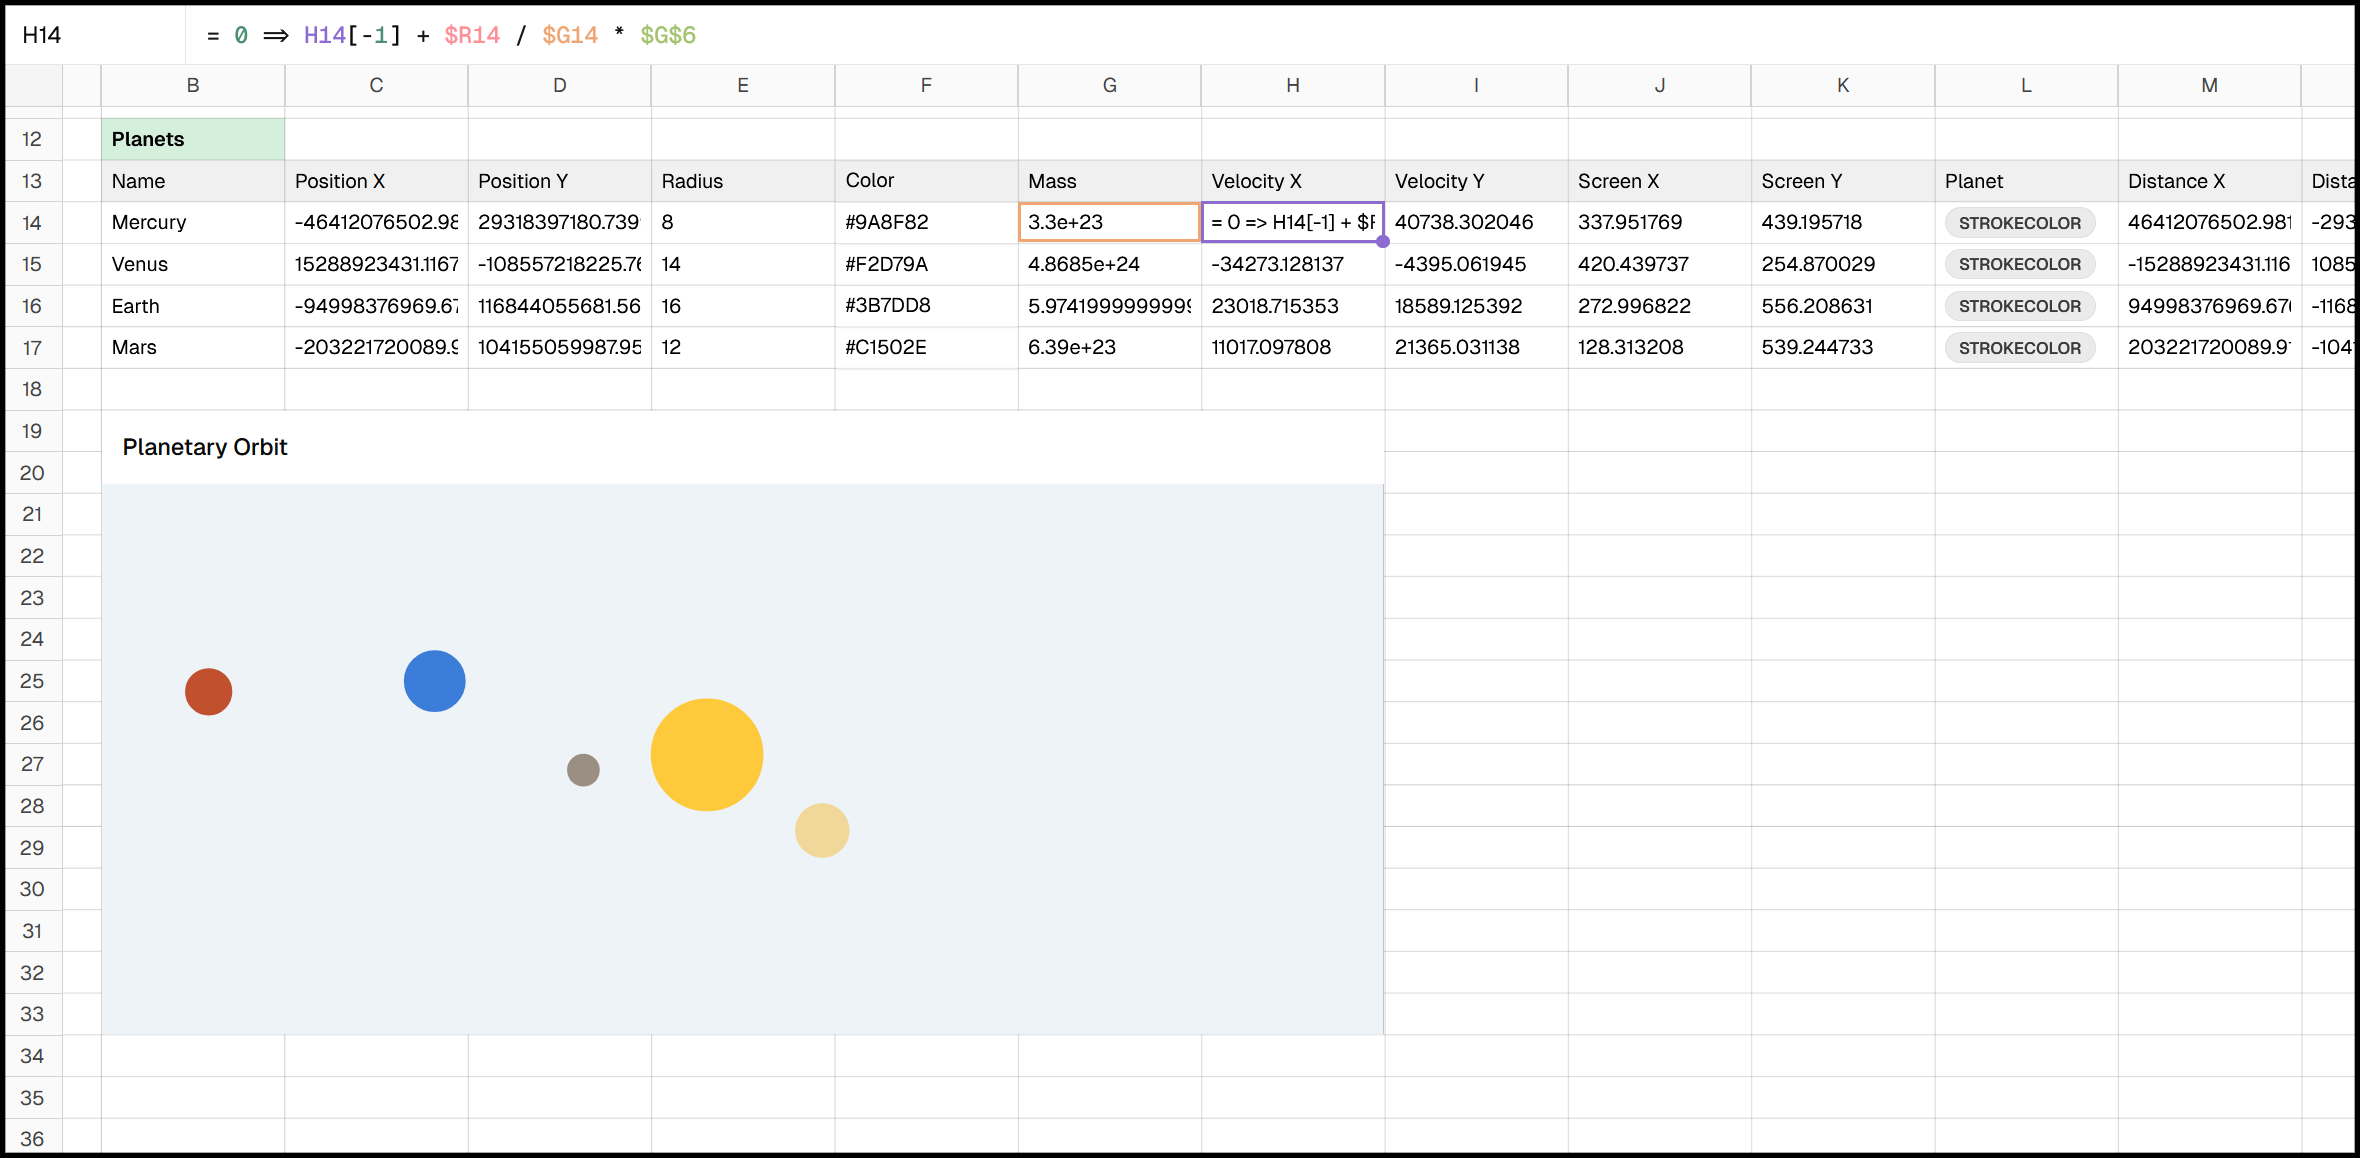
\includegraphics[width=\textwidth]{fig/case-planets}
\caption{Solar system simulation. The displayed table stores attributes of individual planets.}
\label{fig:case-planets}
\vspace{-0.25em}
\end{figure}

\subsubsection*{Spreadsheet structure\DIFaddbegin \DIFadd{.}\DIFaddend }
The spreadsheet consists of four tables. The first one contains constants, such as the astronomical
unit and the gravitational constant. The second and third tables contain information about the
Sun and the planets and the fourth table composes the final visualization by overlaying \DIFdelbegin \DIFdel{black
}\DIFdelend \DIFaddbegin \DIFadd{a light blue
}\DIFaddend background and visual \DIFdelbegin \DIFdel{representation }\DIFdelend \DIFaddbegin \DIFadd{representations }\DIFaddend of the Sun and the planets.

The table with planets (shown in \autoref{fig:case-planets}) records constant information about
each planet (name, radius, mass, color) and information related to the planet's movement.
This is the current distance from the Sun, force applied by the Sun, velocity and position,
kept separately for X and Y coordinates. For the planet Earth, the distance from the Sun and the
applied force are computed as follows (cells \tml{\$M16} and \tml{\$N16} store the X and Y
distances from the Sun, \tml{\$H16} and \tml{\$I16} store the X and Y velocity,
\tml{\$C\$6} is the gravitational constant, \tml{\$G16} is the Earth's mass,
and \tml{\$G\$10} is the Sun's mass; the initial X position is -1 AU while the initial Y
position is 0):

\begin{lstlisting}[style=timelineStyle]
/* Distance */   O16 = SQRT($M16 * $M16 + $N16 * $N16)
/* Force */      P16 = $C$6 * $G16 * $G$10 / POWER($O16, 2)
\end{lstlisting}
\vspace{-0.25em}
\begin{lstlisting}[style=timelineStyle]
/* X Position */ C16 = -1 * $B$6 => C16[-1] + $H16[-1] * $G$6
/* Y Position */ D16 = 0 => D16[-1] + $I16[-1] * $G$6
\end{lstlisting}

\DIFaddbegin \vspace{-0.5em}
\DIFaddend \subsubsection*{Case study assessment\DIFaddbegin \DIFadd{.}\DIFaddend }
\DIFdelbegin \DIFdel{Technically, the }\DIFdelend \DIFaddbegin \DIFadd{The }\DIFaddend case study is similar to the cannonball simulation (\autoref{sec:walkthrough}).
It uses absolute references (dollar sign) to enable the drag down operation for adding further
planets; and it uses \DIFdelbegin \DIFdel{the }\DIFdelend \tml{[-1]} \DIFdelbegin \DIFdel{notation }\DIFdelend to access one past value when updating
the position and velocity. \DIFdelbegin \DIFdel{Because of the large number of attributes needed }\DIFdelend \DIFaddbegin \DIFadd{What it adds to the cannonball example is scale and richer
structure. We keep 18 attributes }\DIFaddend for each planet \DIFdelbegin \DIFdel{,
constructing the same model in a two-dimensional spreadsheet (using rows for time-steps)would be
difficult}\DIFdelend \DIFaddbegin \DIFadd{and the gravitational computation links
every planet to the Sun (we ignore the gravitational forces of other planets).
}

\DIFadd{Representing the simulation in a two dimensions would require one of the workarounds
we observed in the formative study (}\autoref{sec:user-study}\DIFadd{). We could use one wide table and
repeat the same $18$ columns for each planet, or $18$ distinct tables (}\autoref{fig:tables}\DIFadd{).
Both approaches make cross-attribute references and adding more planets awkward.
The difficulty is structurally the same as the one participants encountered when part~(3) of
our study required storing multiple attributes per agent}\DIFaddend .
In \Timeline\DIFaddbegin \DIFadd{, }\DIFaddend the model fits a single \DIFdelbegin \DIFdel{simple table. When constructing the model as well
as the visualization, }\DIFdelend \DIFaddbegin \DIFadd{table, and }\DIFaddend the directness of the \DIFdelbegin \DIFdel{spreadsheet paradigm makes it possible to debug
the formulas
}\DIFdelend \DIFaddbegin \DIFadd{paradigm allows formulas
to be checked against concrete values }\DIFaddend as they are \DIFdelbegin \DIFdel{being }\DIFdelend written.

\DIFaddbegin \begin{figure}
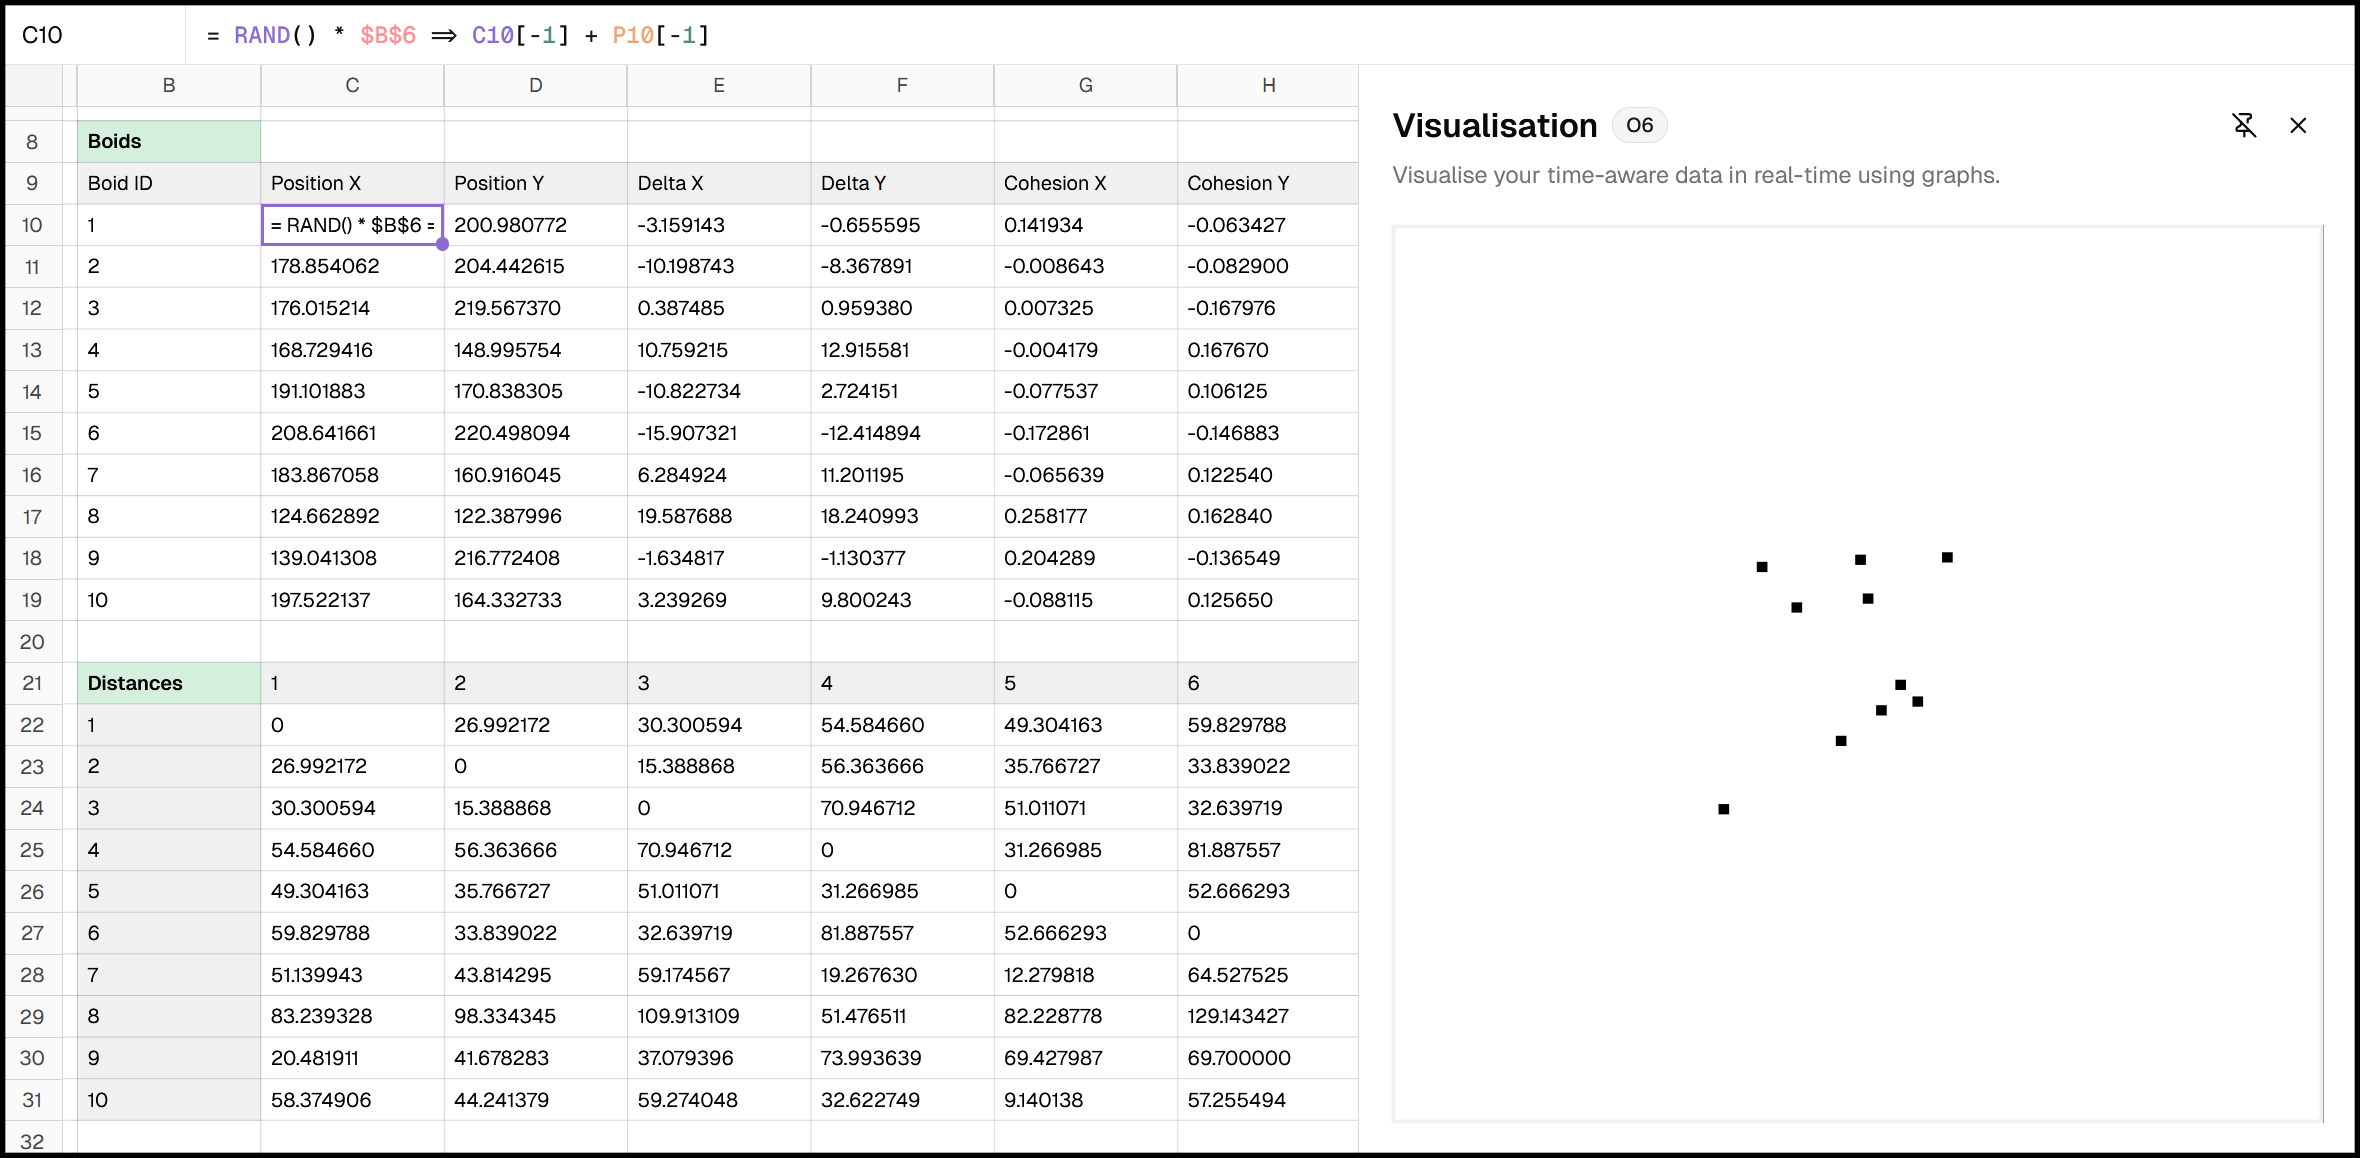
\includegraphics[width=\textwidth]{fig/case-boids}
\caption{\DIFaddFL{Agent-based flocking simulation. The main birds table and an interaction table.}}
\label{fig:case-boids}
\vspace{-0.25em}
\end{figure}

\DIFaddend \subsection{Agent-based flocking simulation}
\label{sec:case-abm}
Our second case study \DIFdelbegin \footnote{\DIFdel{Available at: }%DIFDELCMD < \url{https://timelinesheets.com/spreadsheet/c9b53ee9-0f1b-4d5d-a73e-19f0d201e204}
%DIFDELCMD < %%%
\DIFdel{(same as above)}} %DIFAUXCMD
\addtocounter{footnote}{-1}%DIFAUXCMD
\DIFdelend implements the Boids flocking algorithm \cite{reynolds-1998-boids}
and is inspired by a model developed in Netlogo \cite{wilensky-1998-flocking}. It is an example
of a broad class of agent-based models that are widely used in biology, epidemiology,
behavioral economics and social sciences.

The simulation\DIFaddbegin \footnote{\DIFadd{Available at: }\url{https://timelinesheets.com/spreadsheet/c9b53ee9-0f1b-4d5d-a73e-19f0d201e204}
\DIFadd{(same as above)}} \DIFaddend models the flocking behavior of birds that emerges from the interaction between
individual birds. The birds follow three simple rules: (i) each bird steers away from other birds
in its close proximity, (ii) each bird flies towards the average position of flockmates in its
visual range, and (iii) each bird tries to match the \DIFdelbegin \DIFdel{vector }\DIFdelend \DIFaddbegin \DIFadd{direction and velocity }\DIFaddend of birds in its visual range.

\subsubsection*{Spreadsheet structure\DIFaddbegin \DIFadd{.}\DIFaddend }
The model consists of a table with constants, a table with attributes of the birds and 9
square tables (\DIFdelbegin \DIFdel{no. of birds $\times$ no. }\DIFdelend \DIFaddbegin \DIFadd{$N \times N$ where $N$ is the number }\DIFaddend of birds) that model interactions between birds.
\DIFaddbegin \DIFadd{The 9 tables calculate pairwise distances and various properties based on the distances. The
computation relies on the fact that the tables are aligned and so the drag down operation can be used
to extend a computation for one pair of birds across the entire $N \times N$ table.
}

\DIFaddend \autoref{fig:case-boids} shows the main table and an interaction table calculating the distance
between each pair of birds.
\DIFdelbegin %DIFDELCMD <

%DIFDELCMD < %%%
\DIFdelend The flocking logic is defined in \DIFdelbegin \DIFdel{the main table in }\DIFdelend terms of three properties. Separation
is computed by multiplying the total number of birds in \DIFdelbegin \DIFdel{near }\DIFdelend \DIFaddbegin \DIFadd{close }\DIFaddend proximity by a constant \emph{avoid
factor}. Cohesion is calculated as the average location of birds within \DIFdelbegin \DIFdel{a }\DIFdelend \DIFaddbegin \DIFadd{its }\DIFaddend visual range, multiplied
by the \emph{centering factor}. Finally, alignment is computed as the average X and Y velocity
of birds in the visual range, multiplied by the \emph{matching factor}. The individual
components (\tml{G10}, \tml{I10}, \tml{K10}\DIFaddbegin \DIFadd{, }\tml{U10} \DIFaddend for X and \tml{H10}, \tml{J10}, \tml{L10}\DIFaddbegin \DIFadd{, }\tml{V10} \DIFaddend for Y)
are then added to compute the new speed:

\begin{lstlisting}[style=timelineStyle]
/* Delta X */ E10 = RAND()*10-5 => E10[-1] + G10[-1] + I10[-1] + K10[-1] + U10[-1]
/* Delta Y */ F10 = RAND()*10-5 => F10[-1] + H10[-1] + J10[-1] + L10[-1] + V10[-1]
/* Speed */   O10 = SQRT(E10 * E10 + F10 * F10)
\end{lstlisting}

The interaction between birds is computed in square tables where a cell at relative offset
$i$ and $j$ computes the interaction between a bird at index $i$ and a bird at index $j$.
For example, in the \emph{Distances} table, cell \tml{C23} calculates the distance between the
first bird (position \tml{\$C\$10}, \tml{\$D\$10}) and the second bird (position
\tml{\$C11}, \tml{\$D11}). The cell \tml{C35} in the \emph{Visual Range} table then checks if the
birds are within the visual range of each other (\tml{DIST} is a user-defined helper function):

\begin{lstlisting}[style=timelineStyle]
/* Distances */    C23 = DIST($C11,$D11,$C$10,$D$10)
/* Visual Range */ C35 = IF(AND(C23 != 0, C23 < $D$6), 1, 0)
\end{lstlisting}

\DIFdelbegin %DIFDELCMD < \begin{figure}
%DIFDELCMD < 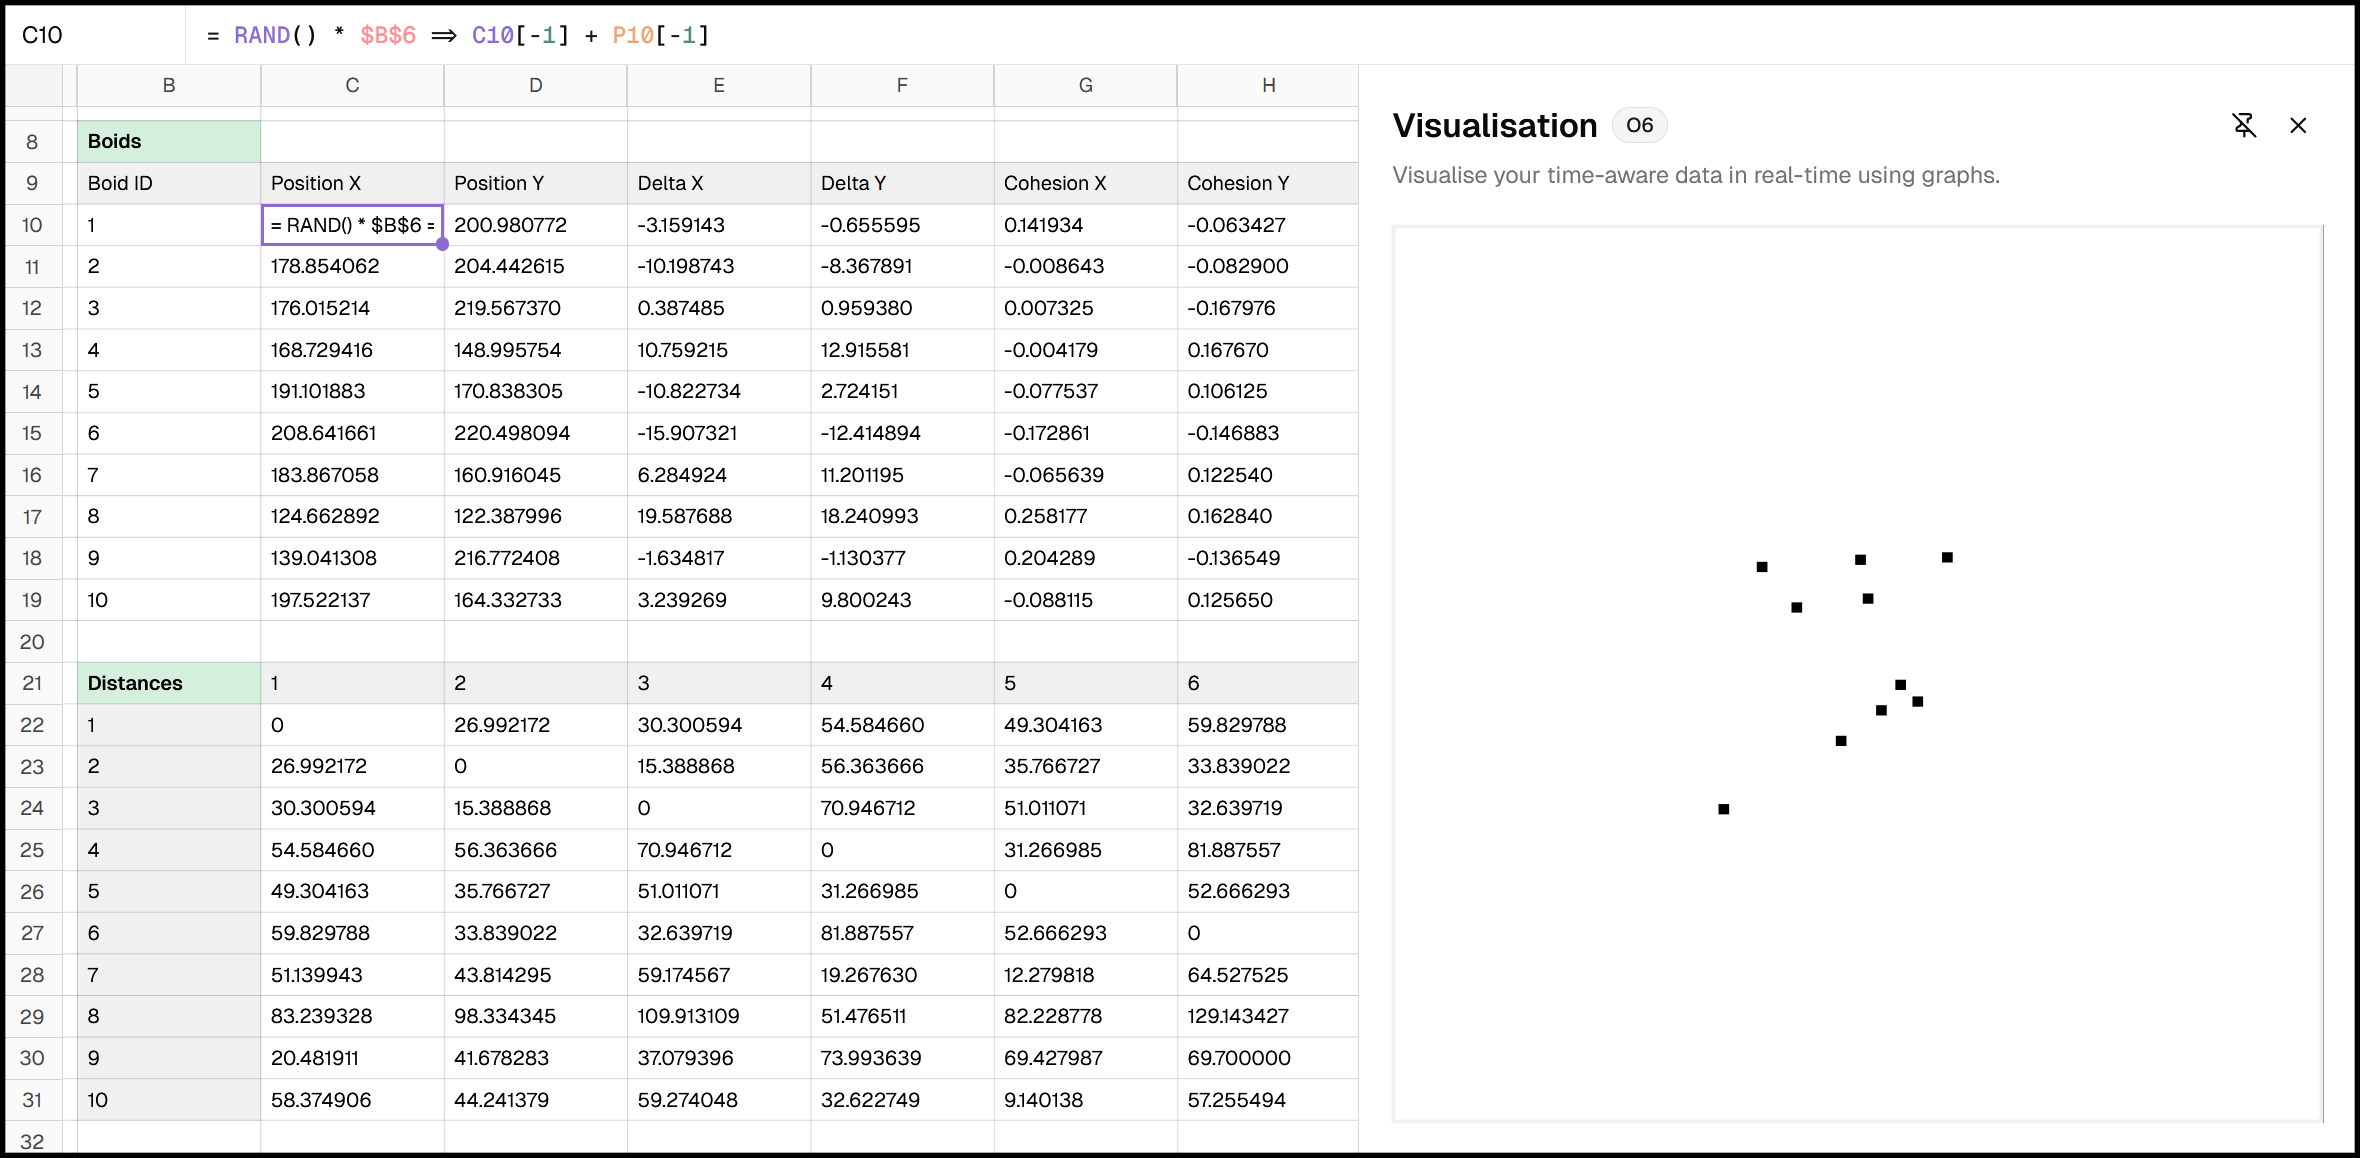
\includegraphics[width=\textwidth]{fig/case-boids}
%DIFDELCMD < %%%
%DIFDELCMD < \caption{%
{%DIFAUXCMD
\DIFdelFL{Agent-based flocking simulation. The main birds table and an interaction table.}}
%DIFAUXCMD
%DIFDELCMD < \label{fig:case-boids}
%DIFDELCMD < \vspace{-0.25em}
%DIFDELCMD < \end{figure}
%DIFDELCMD < %%%
\DIFdelend \DIFaddbegin \subsubsection*{\DIFadd{Case study assessment.}}
\DIFadd{Unlike the previous two case studies, the flocking model uses }\emph{\DIFadd{both}} \DIFadd{spreadsheet dimensions
for its core computation. The $N\times N$ tables model interactions between each pair of birds
and there is no dimension left for time. Using a flat table with $N^2$ columns would make
indexing across tables challenging. The flocking model thus best shows what }\Timeline \DIFadd{enables.
}\DIFaddend

\DIFdelbegin \subsubsection*{\DIFdel{Case study assessment}}
%DIFAUXCMD
\DIFdel{The implementation still relies only on }\DIFdelend \DIFaddbegin \DIFadd{The per-bird logic again uses only }\DIFaddend simple formulas and the \tml{[-1]} construct\DIFdelbegin \DIFdel{to access
previous value of a cell}\DIFdelend ,
but the \DIFdelbegin \DIFdel{sheet is larger. In particular, the construction of
interaction tables requires some effort (we }\DIFdelend \DIFaddbegin \DIFadd{interaction table tracking distances requires more care to construct. We }\DIFaddend can use drag down
to update formulas in one direction \DIFdelbegin \DIFdel{,
}\DIFdelend but not in both, hence \tml{\$C11} has one flexible dimension,
but \tml{\$C\$10} \DIFdelbegin \DIFdel{not in the
}\emph{\DIFdel{Distances}} %DIFAUXCMD
\DIFdel{table)}\DIFdelend \DIFaddbegin \DIFadd{does not}\DIFaddend . In our experience, \DIFdelbegin \DIFdel{interaction tables, as used in this case study,
}\DIFdelend \DIFaddbegin \DIFadd{similar interaction tables
}\DIFaddend are a common design pattern for agent-based models implemented in \Timeline. \DIFaddbegin \DIFadd{Their size grows
quadratically with the number of agents, which bounds the scale of models that remain practical,
but this is a fundamental limitation of spreadsheets.
}\DIFaddend

\subsection{Moving average crossover}
\label{sec:case-finance}

Moving average crossover is a trading strategy that relies on the interaction of a short-term
and a long-term moving average \cite{zakamulin-2025-moving}. When the short-term average crosses
over the long-term average, it suggests a buying opportunity, while the other direction suggests
a possible exit point. Our third case study implements a backtesting algorithm that replays
historical price data and calculates the gains or losses of the strategy over the
history.

\subsubsection*{Spreadsheet structure\DIFaddbegin \DIFadd{.}\DIFaddend }
The spreadsheet (\autoref{fig:case-finance})\footnote{Available at:
\url{https://timelinesheets.com/spreadsheet/e653e57b-9ba9-463d-9f2b-44ddd5a426d3} (same as above)}
loads data from an uploaded CSV file using the \tml{DATASET} function. This is a time-varying
function that returns a value from a row determined by the current time step. In our case,
it replays the history of the price. The computation of the fast and slow moving average looks
at the last 10 and 20 values using a range interval. To detect a crossover, we compare the
relationship in the current and the previous step:

\begin{lstlisting}[style=timelineStyle]
/* Price */   B5 = NUMBER(DATASET("btc", "price"))
/* MA Fast */ B9 = AVERAGE(B5[:-10])
/* MA Slow */ C9 = AVERAGE(B5[:-20])
/* Signal */  D9 = IF(AND(B9>C9,B9[-1]<=C9[-1]),1,IF(AND(B9<C9,B9[-1]>=C9[-1]),-1,0))
\end{lstlisting}

\subsubsection*{Case study assessment\DIFaddbegin \DIFadd{.}\DIFaddend }
\DIFdelbegin \DIFdel{The implementation relies on programming patterns that are common in synchronous dataflow
programming languages, such as the
code }\DIFdelend \DIFaddbegin \DIFadd{Unlike the accumulation-based simulations of the earlier case studies, this example uses the
}\tml{[-1]} \DIFadd{construct }\DIFaddend for edge detection\DIFdelbegin \DIFdel{discussed earlier }\DIFdelend \DIFaddbegin \DIFadd{, which is a pattern common in synchronous dataflow
languages }\DIFaddend (\autoref{sec:features-dataflow}). The example \DIFdelbegin \DIFdel{also utilizes larger history buffer }\DIFdelend \DIFaddbegin \DIFadd{compares the relationship between the
two averages in the current and previous step.
The example also uses larger history buffers }\DIFaddend (10 values for cell \tml{B9}, 20 for \tml{C9}).
These are specified inline and so our analysis can compute the buffer sizes statically.
If the floating window sizes were parameters in the sheet, we would need a more powerful
analysis in order to determine that the value of the cell is constant. The example also illustrates
the power of composable data visualizations, creating sparklines \cite{frishberg-2011-sparklines}
to show the price changes inline.

\begin{figure}
\vspace{-0.5em}
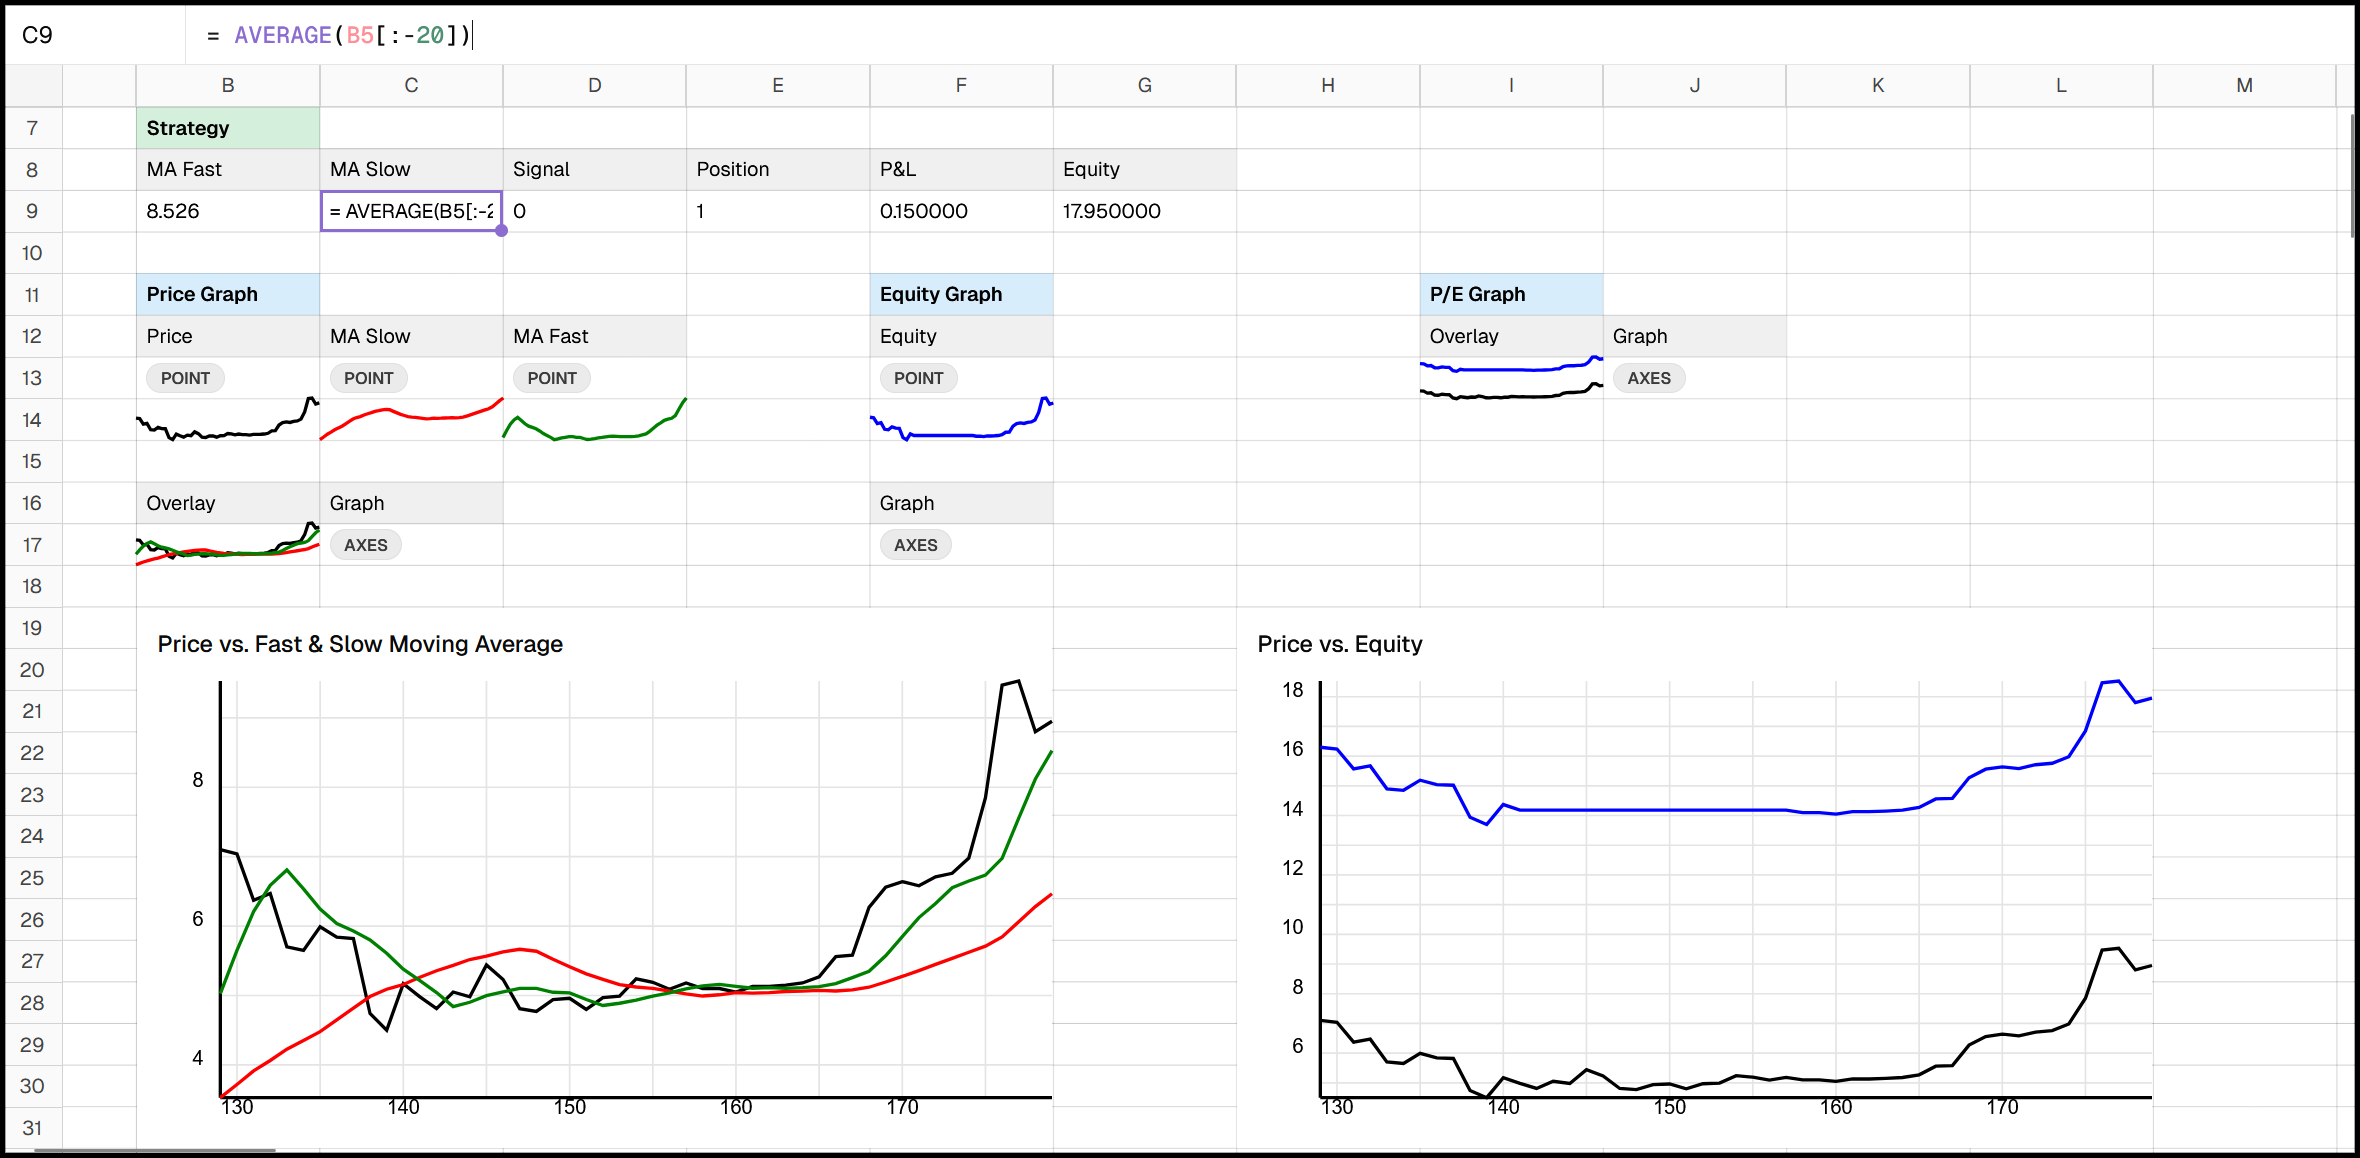
\includegraphics[width=\textwidth]{fig/case-finance}
\vspace{-1em}
\caption{Moving average crossover. Trading strategy and live charts over a floating window.}
\label{fig:case-finance}
\vspace{-0.5em}
\end{figure}

\subsection{Flappy \DIFdelbegin \DIFdel{bird }\DIFdelend \DIFaddbegin \DIFadd{Bird }\DIFaddend game clone\DIFdelbegin %DIFDELCMD < \MBLOCKRIGHTBRACE
%DIFDELCMD < %%%
\DIFdel{Flappy bird }\DIFdelend \DIFaddbegin }
\label{sec:case-flappy}
\DIFadd{Flappy Bird }\DIFaddend is a simple side-scroller game where the player aims to jump through a series of pipes
without hitting them. The bird is dragged down by gravity and jumps up when the user hits a key.

\subsubsection*{Spreadsheet structure\DIFaddbegin \DIFadd{.}\DIFaddend }
Our implementation \DIFaddbegin \DIFadd{(}\DIFaddend \autoref{fig:teaser}\DIFaddbegin \DIFadd{)}\DIFaddend \footnote{Available at: \url{https://timelinesheets.com/spreadsheet/1187c0bd-fe59-4efd-9541-622f35587031} (the web site
does not reveal author identity). To run the game, click \emph{View} $\rightarrow$ \emph{Graph},
click \emph{Play} and then press \texttt{A} to jump.}
contains four tables that define a number of constants (images, map, pipe and bird properties).
The main logic is implemented in two tables that track the positions of the bird and the pipes.
The bird moves down with gravity or up when the keypress is detected using \tml{KEYPRESS("A")}.
The pipes move to the left. A new size and position \DIFdelbegin \DIFdel{is }\DIFdelend \DIFaddbegin \DIFadd{are }\DIFaddend chosen when the pipe moves out of view
and so the table only has a fixed size of 3.

\subsubsection*{Case study assessment\DIFaddbegin \DIFadd{.}\DIFaddend }
The Flappy \DIFdelbegin \DIFdel{bird }\DIFdelend \DIFaddbegin \DIFadd{Bird }\DIFaddend game illustrates the somewhat unexpected capabilities of the \Timeline programming
model, \DIFdelbegin \DIFdel{when }\DIFdelend extended with a simple function to detect key presses. \DIFdelbegin \DIFdel{The discrete }\DIFdelend \DIFaddbegin \DIFadd{Discrete }\DIFaddend time serves as
the main game loop\DIFaddbegin \DIFadd{, }\DIFaddend and composable visualizations can be used to construct the game scene from
individual images (background, bird and pipe sprites).
\DIFdelbegin \DIFdel{As new entries cannot be dynamically }\DIFdelend \DIFaddbegin

\DIFadd{Two aspects point at the limits of the model. First, new rows cannot be }\DIFaddend added to a table \DIFdelbegin \DIFdel{, the existing three pipes }\DIFdelend \DIFaddbegin \DIFadd{dynamically,
so the three pipes are reused as they scroll off-screen. Second, }\Timeline \DIFadd{lacks the higher-order
switching combinators of functional reactive programming (}\autoref{sec:features-frp}\DIFadd{), and so
reset is handled by a condition specified outside of the formula language.
}

\let\thesubsection\oldthesubsection

\section{\DIFadd{Discussion}}
\label{sec:discussion}

\DIFadd{The formative study (}\autoref{sec:user-study}\DIFadd{) identified embedding of
three-dimensional data into a grid as one of the challenges when using conventional
spreadsheets. We first discuss how the grid is used in our case studies (}\autoref{sec:discuss-grid}\DIFadd{)
and then discuss the usability of spreadsheets with time more generally (}\autoref{sec:discuss-usability}\DIFadd{).
}

\subsection{\DIFadd{Working with two dimensions}}
\label{sec:discuss-grid}

\DIFadd{We now revisit the four case studies (}\autoref{sec:case-studies}\DIFadd{), consider how they use the grid
and whether (and how) they could be implemented using an ordinary two-dimensional spreadsheet system:
%DIF >
}\begin{itemize}[itemsep=2mm,topsep=1mm,leftmargin=0.5cm]
\item \DIFadd{Planetary orbit (}\caseref{sec:case-physics}{1}\DIFadd{) and cannonball (}\autoref{sec:walkthrough}\DIFadd{)
  simulations use a table $\textit{entities}\times\textit{attributes}$. To use an ordinary
  spreadsheet, we would need to embed entities and attributes in a single dimension, facing
  the problem discussed earlier (}\autoref{fig:tables}\DIFadd{).
}

\item \DIFadd{Flocking (}\caseref{sec:case-abm}{2}\DIFadd{) uses both an $\textit{entities}\times\textit{attributes}$
  table of size $10\times 17$, but it also uses multiple $\textit{entities}\times \textit{entities}$
  tables for pairwise comparison and other interactions. Doing so in an
  ordinary spreadsheet would require a table with $\textit{entities}^2$ columns and dynamic index calculation.
}

\item \DIFadd{Moving average crossover (}\caseref{sec:case-finance}{3}\DIFadd{) does not use two-dimensional tables
  and could be encoded in an ordinary spreadsheet (using rows for individual values and columns for
  the averages and other computed attributes). The benefit of }\Timeline \DIFadd{is that it can provide a
  live animated chart and could support streaming data. Streaming can be also supported in two-dimensions \mbox{%DIFAUXCMD
\cite{chang-2015-streaming}}\hspace{0pt}%DIFAUXCMD
.
}

\item \DIFadd{Flappy bird (}\caseref{sec:case-flappy}{4}\DIFadd{) also does not use two-dimensional tables,
  but it leverages the fact that the discrete time in }\Timeline \DIFadd{is unbounded (the game can
  continue indefinitely) and that keyboard events can be used as inputs. This could
  also be achieved in a two-dimensional model \mbox{%DIFAUXCMD
\cite{chang-2015-streaming,chang-2014-web}}\hspace{0pt}%DIFAUXCMD
.
}\end{itemize}

\DIFadd{Implementing the first three case studies in an ordinary spreadsheet system is possible, but
it would require large amount of space, especially for }\caseref{sec:case-abm}{2}\DIFadd{. This is
a situation encountered in part 3 of our formative study that two of the participants judged as
}\emph{\DIFadd{miserable}} \DIFadd{and }\emph{\DIFadd{painful}}\DIFadd{, respectively.
}

\subsection{\DIFadd{Usability of spreadsheets with time}}
\label{sec:discuss-usability}

\DIFadd{Spreadsheets are a canonical example of end-user programming tool
\mbox{%DIFAUXCMD
\cite{ko-2011-enduser,nardi-1993-matter}}\hspace{0pt}%DIFAUXCMD
, but the question why and how exactly
spreadsheets achieve their usability does not have an established answer.
We review existing analyses and discuss what they suggest about the usability of }\Timeline\DIFadd{.
}

\subsubsection*{\DIFadd{Evaluating spreadsheet systems.}}
\DIFadd{Many analyses of spreadsheets focus on documenting their errors and engineering limitations
\mbox{%DIFAUXCMD
\cite{hermans-2015-smells,panko-1998-errors}}\hspace{0pt}%DIFAUXCMD
. A few analyses attempt to explain what makes
spreadsheets work. Nardi \mbox{%DIFAUXCMD
\cite{nardi-1993-matter} }\hspace{0pt}%DIFAUXCMD
argues that spreadsheets
succeed because they closely fit the domain of tabular data analysis, while not requiring
explicit control flow and abstraction. Spreadsheets also achieve a high degree of liveness,
due to the edit-triggered recomputation \mbox{%DIFAUXCMD
\cite{tanimoto-2013-live}}\hspace{0pt}%DIFAUXCMD
.
}

\DIFadd{A more structured analysis of spreadsheets \mbox{%DIFAUXCMD
\cite{hendry-1994-spreadsheets} }\hspace{0pt}%DIFAUXCMD
has been done
using the cognitive dimensions of notations framework \mbox{%DIFAUXCMD
\cite{green-1996-cogdims}}\hspace{0pt}%DIFAUXCMD
. It
identified several notable characteristics. Spreadsheets support }\emph{\DIFadd{closeness of mapping}}\DIFadd{.
If the problem naturally has a two-dimensional strucutre, the problem domain fits with the program
domain. They do not suffer from high }\emph{\DIFadd{viscosity}}\DIFadd{, meaning that changes are
easy to make (even if this requires copying the modified formula). However, spreadsheets suffer
from poor }\emph{\DIFadd{visibility}} \DIFadd{of code and }\emph{\DIFadd{hidden dependencies}}\DIFadd{, because logic is hidden inside formulas
that }\DIFaddend have to be \DIFdelbegin \DIFdel{reused}\DIFdelend \DIFaddbegin \DIFadd{explicitly viewed. The analysis also attributes the success of spreadsheets to their
low }\emph{\DIFadd{abstraction level}} \DIFadd{and support for }\emph{\DIFadd{progressive evaluation}}\DIFadd{, i.e., live immediate feedback.
The analysis provides a limited baseline for heuristic evaluation of spreadsheet extensions.
}

\subsubsection*{\DIFadd{Adding the time dimension.}}
\DIFadd{Applying Nardi's analysis to }\Timeline \DIFadd{suggests that spreadsheets with discrete time fit
a broader range of application domains. In addition to tabular data analysis, these
include the four domains discussed above (}\autoref{sec:case-studies}\DIFadd{) and so }\Timeline \DIFadd{can
achieve better }\emph{\DIFadd{closeness of mapping}} \DIFadd{by not requiring an auxiliary tables
(}\autoref{fig:tables}\DIFadd{) to store values. The system also preserves a high degree of liveness through
edit-triggered recomputation.
}

\DIFadd{Reference to values in earlier steps, such as }\tml{A1[-1]}\DIFadd{, are less direct because the value
of }\tml{A1[-1]} \DIFadd{is not readily displayed in the grid and
cannot be referenced by clicking on it when writing a formula. This property is not
identified by aformentioned analyses, but relates to }\emph{\DIFadd{concrete programming}}
\DIFadd{\mbox{%DIFAUXCMD
\cite{edwards-2004-concrete}}\hspace{0pt}%DIFAUXCMD
. Programming in }\Timeline \DIFadd{is thus less concrete than in ordinary
spreadsheets.
}

\Timeline \DIFadd{has a higher }\emph{\DIFadd{viscosity}} \DIFadd{than conventional spreadsheets when the user wants
to modify a value at certain time steps. When encoding time as rows, this can be done by selecting
the affected range and modifying the value. In }\Timeline\DIFadd{,
such change can only be done by using }\tml{IF} \DIFadd{function with a condition based on the current
}\tml{STEP()}\DIFadd{.
Modifying the logic for all time steps is easier in }\Timeline\DIFadd{, where it
exists in a single formula, as opposed to multiple copies of the same formula.
}

\DIFadd{The }\emph{\DIFadd{visibility}} \DIFadd{of code remains unchanged, but }\emph{\DIFadd{visibility}} \DIFadd{of computed values
is decreased because only values for a single time step are displayed. (When representing time
as rows, multiple time steps are visible.) To alleviate this limitation, }\Timeline \DIFadd{makes it
easy to construct sparklines as shown in the financial analysis (}\caseref{sec:case-finance}{3}\DIFadd{),
which make previous values visible in a concise form.
}

\subsubsection*{\DIFadd{The limits of discrete time.}}
\Timeline \DIFadd{uses discrete time, which limits what kind of models it can express.
The grid is fixed and entities cannot be created over time. A flocking simulation with
constant number of birds (}\caseref{sec:case-abm}{2}\DIFadd{) is expressible, but a predator-prey model
in which individuals are born and die can only be modelled by pre-allocating a table of
entities. Moreover, }\Timeline \DIFadd{has no analogue of the
clock calculi of synchronous languages \mbox{%DIFAUXCMD
\cite{caspi-1992-clocks}}\hspace{0pt}%DIFAUXCMD
, which would allow cells to progress
at different rates. Supporting a more general notion of discrete time would be useful in domains such
as finance where users often work with data indexed by time. Generalising the notion of time
would require adapting not just the evaluation model, but also the indexing logic and notation}\DIFaddend .

\section{Related work}
\Timeline shows that a large number of programming language research
concepts are directly applicable to spreadsheets. Earlier discussion (\autoref{sec:features})
covers work on \DIFdelbegin \DIFdel{coeffect systems, data visualization and typed holes}\DIFdelend \DIFaddbegin \DIFadd{coeffects, functional reactive programming and visualization}\DIFaddend . This section
\DIFdelbegin \DIFdel{provides an overview of }\DIFdelend \DIFaddbegin \DIFadd{reviews }\DIFaddend the remaining main related research areas.

\DIFdelbegin %DIFDELCMD < \vspace{-0.25em}
%DIFDELCMD < %%%
\DIFdelend \subsubsection*{Extending the spreadsheet model\DIFaddbegin \DIFadd{.}\DIFaddend }
Forms/3~\cite{burnett-2001-forms3} is a pioneering extension of spreadsheets to non-tabular
format, that inspired later work \cite{bazant-2018-nontabular}; spreadsheets have been extended
to support object-orientation \cite{mccutchen-2016-oop,clack-1997-object} and
programming by demonstration \cite{gulwani-2012-examples}. An early attempt
to use spreadsheets for interactive graphics is by Wilde et al. \cite{wilde-1990-graphics}.
Websheets~\cite{chang-2014-web} and streaming extensions~\cite{chang-2015-streaming} integrate
spreadsheets with live data (but without adding a third dimension). Spreadsheets served as
an inspiration for multiple other languages \cite{yoder-1994-real,petricek-2022-gamma}.
Cuscus is a design prototype for describing rich visualizations in a
spreadsheet~\cite{marasoiu-2019-cuscus} and our work has also been inspired by
sparklines~\cite{frishberg-2011-sparklines}.

\DIFdelbegin %DIFDELCMD < \vspace{-0.2em}
%DIFDELCMD < %%%
\DIFdelend \subsubsection*{Abstractions and types for spreadsheets\DIFaddbegin \DIFadd{.}\DIFaddend }
Sheet-defined functions are introduced in~\cite{jones-2003-functions} with formal semantics
developed later~\cite{sestoft-2013-sheetdef,bock-2020-sheetdef,bock-2022-cost}. Later work allows
variable-size input~\cite{mccutchen-2020-sdfs}, while gridlets \cite{joharizadeh-2020-gridlets}
serve as reusable sheet blocks and have been implemented using spilled arrays~\cite{williams-2020-spilled},
which directly inspired our semantics. Multiple systems provide static type systems for
spreadsheets~\cite{ahmad-2003-types,abraham-2006-types}, perform static analysis of formulas
\cite{cheng-2015-static} or apply other software engineering techniques \cite{hermans-2016-spreadsheets}.

\DIFdelbegin %DIFDELCMD < \vspace{-0.2em}
%DIFDELCMD < %%%
\DIFdelend \subsubsection*{Dataflow and functional reactive programming\DIFaddbegin \DIFadd{.}\DIFaddend }
The \Timeline execution draws inspiration from synchronous dataflow languages
\DIFdelbegin \DIFdel{such as
Lucid, Lustre and Esterel~}\DIFdelend \cite{benveniste-2003-sync,ashcroft-1977-lucid,caspi-1987-lustre,halbwachs-1991-lustre,berry-1992-esterel}.
Our programming model is most closely related to Lustre, whose clock calculus~\cite{caspi-1992-clocks}
\DIFdelbegin \DIFdel{is a predecessor of }\DIFdelend \DIFaddbegin \DIFadd{resembles }\DIFaddend our checking of past accesses. Functional reactive programming systems
\cite{elliott-1997-fran,wan-2000-frp,courtney-2003-yampa} do not use discrete time\DIFdelbegin \DIFdel{, but
}\DIFdelend \DIFaddbegin \DIFadd{;
}\DIFaddend event-based \DIFdelbegin \DIFdel{systems are }\DIFdelend \DIFaddbegin \DIFadd{functional reactive programming is }\DIFaddend more similar to our approach \cite{wan-2002-efrp}.
\DIFdelbegin \DIFdel{Space leak problems have been a challenge for the implementation of FRP
systems~\mbox{%DIFAUXCMD
\cite{krishnaswami-2013-leaks,bahr-2022-frp}}\hspace{0pt}%DIFAUXCMD
, not shared by our system.
}\DIFdelend

\DIFdelbegin %DIFDELCMD < \vspace{-0.2em}
%DIFDELCMD < %%%
\DIFdelend \subsubsection*{Semantics of reactive and dataflow programs\DIFaddbegin \DIFadd{.}\DIFaddend }
Our semantics has been inspired by operational approaches \cite{williams-2020-spilled,bock-2020-sheetdef,bock-2022-cost}.
More dynamic reactive systems often use graph-based evaluation \cite{satyanarayan-2016-vega,oeyen-2023-graphbased}.
The semantics of dataflow languages has been given in both monadic~\cite{wadge-1995-monads}
and comonadic style~\cite{uustalu-2006-essence}.
The semantics of functional reactive programming languages has been
defined denotationally \cite{elliott-2009-pushpull} using a range of categorical
models \cite{jeltsch-2014-categorical,krishnaswami-2011-ultra}, but recently also in an
operational style \cite{ischard-2025-frp}.

\DIFdelbegin %DIFDELCMD < \vspace{-0.3em}
%DIFDELCMD < %%%
\DIFdelend \section{Conclusions}
Spreadsheets are the most widely used programming systems in the world, but their expressive
power is limited. Attempts to extend spreadsheets face a challenge---how to extend the power
of the programming model, without losing their liveness, directness and usability?
\Timeline shows that adding a time dimension to spreadsheets keeps their desirable properties,
but makes them more powerful. Spreadsheets with time can be used to implement agent-based
models, physics simulations, financial analyses and even interactive games.

\DIFdelbegin \DIFdel{The key observation in this paper is that }\DIFdelend \DIFaddbegin \DIFadd{Technically, }\DIFaddend the design and implementation of a spreadsheet system
with time can draw on a rich body of programming languages research. Our execution model takes
inspiration from synchronous dataflow languages and functional reactive programming, we
guarantee memory-bounded execution using coeffects, \DIFdelbegin \DIFdel{the formula editor can leverage the theory of
typed holes }\DIFdelend and we can support rich charts by using ideas
rooted in grammar of graphics. There is more to spreadsheets than meets the (programming language
researcher's)\DIFaddbegin \DIFadd{~}\DIFaddend eye!

%DIF > TODO: ACKS: Clemens, Vít Ungermann, Raphael Wimmer, Jakob Haimerl and Tobias Wittl
%DIF >  \footnote{We thank anonymous reviewer for pointing out the mid-air change scenario.}
\DIFaddbegin

\DIFaddend \newpage
\section*{Data availability statement}
An implementation of \Timeline will be submitted as an artifact, consisting of:
\begin{itemize}[itemsep=0mm,topsep=1mm,leftmargin=0.5cm]
  \item[--] Stand-alone package that can be used to run \Timeline locally (Docker image)
  \item[--] Easily accessible implementation of the four case studies discussed in the paper
    (Flappy \DIFdelbegin \DIFdel{bird}\DIFdelend \DIFaddbegin \DIFadd{Bird}\DIFaddend , Moving average crossover, Flocking simulation, Solar system simulation)
    and the introductory example (Cannonball simulation).
\end{itemize}

\noindent
The artifact differs from the fully general theoretical account provided in the paper in that:
\begin{itemize}[itemsep=0mm,topsep=1mm,leftmargin=0.5cm]
  \item[--] The implementation of cell evaluation is based on topological ordering of dependencies
    and update propagation. This aspect is left unspecified in this paper.
  \item[--] All the examples and case studies work exactly as described in the paper. Some may use
    advanced features for readability (such as named ranges and user-defined functions).
  \item[--] The system implements only the simple mechanism for checking the required number of
    past values (without the coeffect-based optimization). Coeffect-based model is theoretically
    interesting, but not necessary for efficiency in practice.
  \item[--] The execution using bounded memory can be enabled or disabled (it saves memory,
    but makes it difficult to go to the previous step, which is helpful for debugging)
  \item[--] Formula editing based on holes is not implemented. Currently, \Timeline inserts
    a cell reference on click when \texttt{Ctrl} is pressed. Implementing the theory described
    in the paper is future work.
\end{itemize}


\section*{Generative AI tools use}
The system implementation and the paper have been solely written by the authors.
Generative AI tools (Claude Code, \url{https://claude.ai}) has been used while writing and revising
the paper: (i) as a critic of the paper text (prompted to find flaws, omissions and inconsistencies),
(ii) to generate ideas on possible ways of structuring and framing some of the sections in the paper
(prompted to suggest possible options), and (iii) for langauge corrections and spellchecking (prompted to
list issues). In all cases, the authors wrote the actual text as it appears in the paper.


%\begin{acks}
%Omitted
%thanks to Mickael for pointing out the synchronous languages link!
%DIF > thanks to Vit Ungermann for adding compost
%\end{acks}

\bibliographystyle{ACM-Reference-Format}
\DIFdelbegin %DIFDELCMD < \bibliography{main}
%DIFDELCMD < %%%
\DIFdelend %DIF > %% -*-BibTeX-*-
%DIF > %% Do NOT edit. File created by BibTeX with style
%DIF > %% ACM-Reference-Format-Journals [18-Jan-2012].
\DIFaddbegin

\begin{thebibliography}{73}

%DIF > %% ====================================================================
%DIF > %% NOTE TO THE USER: you can override these defaults by providing
%DIF > %% customized versions of any of these macros before the \bibliography
%DIF > %% command.  Each of them MUST provide its own final punctuation,
%DIF > %% except for \shownote{} and \showURL{}.  The latter two
%DIF > %% do not use final punctuation, in order to avoid confusing it with
%DIF > %% the Web address.
%DIF > %%
%DIF > %% To suppress output of a particular field, define its macro to expand
%DIF > %% to an empty string, or better, \unskip, like this:
%DIF > %%
%DIF > %% \newcommand{\showURL}[1]{\unskip}   % LaTeX syntax
%DIF > %%
%DIF > %% \def \showURL #1{\unskip}           % plain TeX syntax
%DIF > %%
%DIF > %% ====================================================================

\ifx \showCODEN    \undefined \def \showCODEN     \DIFadd{#1}{\unskip}     \fi
\ifx \showISBNx    \undefined \def \showISBNx     \DIFadd{#1}{\unskip}     \fi
\ifx \showISBNxiii \undefined \def \showISBNxiii  \DIFadd{#1}{\unskip}     \fi
\ifx \showISSN     \undefined \def \showISSN      \DIFadd{#1}{\unskip}     \fi
\ifx \showLCCN     \undefined \def \showLCCN      \DIFadd{#1}{\unskip}     \fi
\ifx \shownote     \undefined \def \shownote      \DIFadd{#1}{\DIFadd{#1}}          \fi
\ifx \showarticletitle \undefined \def \showarticletitle \DIFadd{#1}{\DIFadd{#1}}   \fi
\ifx \showURL      \undefined \def \showURL       {\relax}        \fi
%DIF >  The following commands are used for tagged output and should be
%DIF >  invisible to TeX
\providecommand\bibfield[2]{#2}
\providecommand\bibinfo[2]{#2}
\providecommand\natexlab[1]{#1}
\providecommand\showeprint[2][]{arXiv:#2}

\bibitem[Abar et~al\mbox{.}(2017)]%DIF >
        {\DIFadd{abar-2017-abm}}
\bibfield{author}{\bibinfo{person}{Sameera Abar}, \bibinfo{person}{Georgios~K.
  Theodoropoulos}, \bibinfo{person}{Pierre Lemarinier}, {and}
  \bibinfo{person}{Gregory~M.P. O’Hare}.} \bibinfo{year}{2017}\natexlab{}\DIFadd{.
}\newblock \showarticletitle{Agent Based Modelling and Simulation tools: A
  review of the state-of-art software}\DIFadd{.
}\newblock \bibinfo{journal}{\emph{Computer Science Review}}
  \bibinfo{volume}{24} \DIFadd{(}\bibinfo{year}{2017}\DIFadd{), }\bibinfo{pages}{13--33}\DIFadd{.
}\newblock
\showISSN{1574-0137}
\href{https://doi.org/10.1016/j.cosrev.2017.03.001}{doi:\nolinkurl{10.1016/j.cosrev.2017.03.001}}


\bibitem[Abraham et~al\mbox{.}(2009)]%DIF >
        {\DIFadd{abraham-2009-prog}}
\bibfield{author}{\bibinfo{person}{Robin Abraham}, \bibinfo{person}{Margaret
  Burnett}, {and} \bibinfo{person}{Martin Erwig}.}
  \bibinfo{year}{2009}\natexlab{}\DIFadd{.
}\newblock \bibinfo{booktitle}{\emph{Spreadsheet Programming}}\DIFadd{.
}\newblock \bibinfo{publisher}{John Wiley \& Sons, Ltd}\DIFadd{,
  }\bibinfo{pages}{2804--2810}\DIFadd{.
}\newblock
\showISBNx{9780470050118}
\href{https://doi.org/10.1002/9780470050118.ecse415}{doi:\nolinkurl{10.1002/9780470050118.ecse415}}


\bibitem[Abraham and Erwig(2006)]%DIF >
        {\DIFadd{abraham-2006-types}}
\bibfield{author}{\bibinfo{person}{Robin Abraham} {and} \bibinfo{person}{Martin
  Erwig}.} \bibinfo{year}{2006}\natexlab{}\DIFadd{.
}\newblock \showarticletitle{Type inference for spreadsheets}\DIFadd{. In
  }\bibinfo{booktitle}{\emph{Proceedings of the 8th ACM SIGPLAN International
  Conference on Principles and Practice of Declarative Programming}} \DIFadd{(Venice,
  Italy) }\emph{\DIFadd{(}\bibinfo{series}{PPDP '06}\DIFadd{)}}\DIFadd{. }\bibinfo{publisher}{Association
  for Computing Machinery}\DIFadd{, }\bibinfo{address}{New York, NY, USA}\DIFadd{,
  }\bibinfo{pages}{73–84}\DIFadd{.
}\newblock
\showISBNx{1595933883}
\href{https://doi.org/10.1145/1140335.1140346}{doi:\nolinkurl{10.1145/1140335.1140346}}


\bibitem[Ahmad et~al\mbox{.}(2003)]%DIF >
        {\DIFadd{ahmad-2003-types}}
\bibfield{author}{\bibinfo{person}{Y. Ahmad}, \bibinfo{person}{T. Antoniu},
  \bibinfo{person}{S. Goldwater}, {and} \bibinfo{person}{S. Krishnamurthi}.}
  \bibinfo{year}{2003}\natexlab{}\DIFadd{.
}\newblock \showarticletitle{A type system for statically detecting spreadsheet
  errors}\DIFadd{. In }\bibinfo{booktitle}{\emph{18th IEEE International Conference on
  Automated Software Engineering, 2003. Proceedings.}}
  \bibinfo{pages}{174--183}\DIFadd{.
}\newblock
\href{https://doi.org/10.1109/ASE.2003.1240305}{doi:\nolinkurl{10.1109/ASE.2003.1240305}}


\bibitem[Ahmed(2006)]%DIF >
        {\DIFadd{ahmed-2006-stepindexed}}
\bibfield{author}{\bibinfo{person}{Amal Ahmed}.}
  \bibinfo{year}{2006}\natexlab{}\DIFadd{.
}\newblock \showarticletitle{Step-Indexed Syntactic Logical Relations for
  Recursive and Quantified Types}\DIFadd{. In }\bibinfo{booktitle}{\emph{Programming
  Languages and Systems}}\DIFadd{, }\bibfield{editor}{\bibinfo{person}{Peter Sestoft}}
  \DIFadd{(Ed.). }\bibinfo{publisher}{Springer Berlin Heidelberg}\DIFadd{,
  }\bibinfo{address}{Berlin, Heidelberg}\DIFadd{, }\bibinfo{pages}{69--83}\DIFadd{.
}\newblock
\showISBNx{978-3-540-33096-7}


\bibitem[Ashcroft and Wadge(1977)]%DIF >
        {\DIFadd{ashcroft-1977-lucid}}
\bibfield{author}{\bibinfo{person}{Edward~A. Ashcroft} {and}
  \bibinfo{person}{William~W. Wadge}.} \bibinfo{year}{1977}\natexlab{}\DIFadd{.
}\newblock \showarticletitle{{Lucid}, a Nonprocedural Language with Iteration}\DIFadd{.
}\newblock \bibinfo{journal}{\emph{Commun. ACM}} \bibinfo{volume}{20}\DIFadd{,
  }\bibinfo{number}{7} \DIFadd{(}\bibinfo{year}{1977}\DIFadd{), }\bibinfo{pages}{519--526}\DIFadd{.
}\newblock
\href{https://doi.org/10.1145/359636.359715}{doi:\nolinkurl{10.1145/359636.359715}}


\bibitem[Bahr(2022)]%DIF >
        {\DIFadd{bahr-2022-frp}}
\bibfield{author}{\bibinfo{person}{Patrick Bahr}.}
  \bibinfo{year}{2022}\natexlab{}\DIFadd{.
}\newblock \showarticletitle{Modal {FRP} for all: Functional reactive
  programming without space leaks in {Haskell}}\DIFadd{.
}\newblock \bibinfo{journal}{\emph{Journal of Functional Programming}}
  \bibinfo{volume}{32} \DIFadd{(}\bibinfo{year}{2022}\DIFadd{), }\bibinfo{pages}{e15}\DIFadd{.
}\newblock
\href{https://doi.org/10.1017/S0956796822000132}{doi:\nolinkurl{10.1017/S0956796822000132}}


\bibitem[Ba{\v z}ant and Mar{\v s}{\'a}lkov{\'a}(2018)]%DIF >
        {\DIFadd{bazant-2018-nontabular}}
\bibfield{author}{\bibinfo{person}{Pavel Ba{\v z}ant} {and}
  \bibinfo{person}{Michaela Mar{\v s}{\'a}lkov{\'a}}.}
  \bibinfo{year}{2018}\natexlab{}\DIFadd{.
}\newblock \showarticletitle{A Non-Tabular Spreadsheet with Broad
  Applicability}\DIFadd{. In }\bibinfo{booktitle}{\emph{Companion {{Proceedings}} of the
  2nd {{International Conference}} on the {{Art}}, {{Science}}, and
  {{Engineering}} of {{Programming}}}} \emph{\DIFadd{(}\bibinfo{series}{Programming
  '18}\DIFadd{)}}\DIFadd{. }\bibinfo{publisher}{Association for Computing Machinery}\DIFadd{,
  }\bibinfo{address}{New York, NY, USA}\DIFadd{, }\bibinfo{pages}{161--165}\DIFadd{.
}\newblock
\showISBNx{978-1-4503-5513-1}
\href{https://doi.org/10.1145/3191697.3214343}{doi:\nolinkurl{10.1145/3191697.3214343}}


\bibitem[Benveniste et~al\mbox{.}(2003)]%DIF >
        {\DIFadd{benveniste-2003-sync}}
\bibfield{author}{\bibinfo{person}{A. Benveniste}, \bibinfo{person}{P. Caspi},
  \bibinfo{person}{S.A. Edwards}, \bibinfo{person}{N. Halbwachs},
  \bibinfo{person}{P. Le~Guernic}, {and} \bibinfo{person}{R. de Simone}.}
  \bibinfo{year}{2003}\natexlab{}\DIFadd{.
}\newblock \showarticletitle{The synchronous languages 12 years later}\DIFadd{.
}\newblock \bibinfo{journal}{\emph{Proc. IEEE}} \bibinfo{volume}{91}\DIFadd{,
  }\bibinfo{number}{1} \DIFadd{(}\bibinfo{year}{2003}\DIFadd{), }\bibinfo{pages}{64--83}\DIFadd{.
}\newblock
\href{https://doi.org/10.1109/JPROC.2002.805826}{doi:\nolinkurl{10.1109/JPROC.2002.805826}}


\bibitem[Berry and Gonthier(1992)]%DIF >
        {\DIFadd{berry-1992-esterel}}
\bibfield{author}{\bibinfo{person}{G{\'e}rard Berry} {and}
  \bibinfo{person}{Georges Gonthier}.} \bibinfo{year}{1992}\natexlab{}\DIFadd{.
}\newblock \showarticletitle{The {Esterel} Synchronous Programming Language:
  Design, Semantics, Implementation}\DIFadd{.
}\newblock \bibinfo{journal}{\emph{Science of Computer Programming}}
  \bibinfo{volume}{19}\DIFadd{, }\bibinfo{number}{2} \DIFadd{(}\bibinfo{year}{1992}\DIFadd{),
  }\bibinfo{pages}{87--152}\DIFadd{.
}\newblock
\href{https://doi.org/10.1016/0167-6423(92)90005-V}{doi:\nolinkurl{10.1016/0167-6423(92)90005-V}}


\bibitem[Bock et~al\mbox{.}(2022)]%DIF >
        {\DIFadd{bock-2022-cost}}
\bibfield{author}{\bibinfo{person}{Alexander~Asp Bock}, \bibinfo{person}{Thomas
  B{\o}gholm}, \bibinfo{person}{Peter Sestoft}, \bibinfo{person}{Bent Thomsen},
  {and} \bibinfo{person}{Lone~Leth Thomsen}.} \bibinfo{year}{2022}\natexlab{}\DIFadd{.
}\newblock \showarticletitle{On the cost semantics for spreadsheets with
  sheet-defined functions}\DIFadd{.
}\newblock \bibinfo{journal}{\emph{J. Comput. Lang.}}  \bibinfo{volume}{69}
  \DIFadd{(}\bibinfo{year}{2022}\DIFadd{), }\bibinfo{pages}{101103}\DIFadd{.
}\newblock
\href{https://doi.org/10.1016/J.COLA.2022.101103}{doi:\nolinkurl{10.1016/J.COLA.2022.101103}}


\bibitem[Bock et~al\mbox{.}(2020)]%DIF >
        {\DIFadd{bock-2020-sheetdef}}
\bibfield{author}{\bibinfo{person}{Alexander~Asp Bock}, \bibinfo{person}{Thomas
  Bøgholm}, \bibinfo{person}{Peter Sestoft}, \bibinfo{person}{Bent Thomsen},
  {and} \bibinfo{person}{Lone~Leth Thomsen}.} \bibinfo{year}{2020}\natexlab{}\DIFadd{.
}\newblock \showarticletitle{On the semantics for spreadsheets with
  sheet-defined functions}\DIFadd{.
}\newblock \bibinfo{journal}{\emph{Journal of Computer Languages}}
  \bibinfo{volume}{57} \DIFadd{(}\bibinfo{year}{2020}\DIFadd{), }\bibinfo{pages}{100960}\DIFadd{.
}\newblock
\showISSN{2590-1184}
\href{https://doi.org/10.1016/j.cola.2020.100960}{doi:\nolinkurl{10.1016/j.cola.2020.100960}}


\bibitem[Brunel et~al\mbox{.}(2014)]%DIF >
        {\DIFadd{brunel-2014-coeffects}}
\bibfield{author}{\bibinfo{person}{Alo{\"i}s Brunel}, \bibinfo{person}{Marco
  Gaboardi}, \bibinfo{person}{Damiano Mazza}, {and} \bibinfo{person}{Steve
  Zdancewic}.} \bibinfo{year}{2014}\natexlab{}\DIFadd{.
}\newblock \showarticletitle{A Core Quantitative Coeffect Calculus}\DIFadd{. In
  }\bibinfo{booktitle}{\emph{Programming Languages and Systems}}\DIFadd{,
  }\bibfield{editor}{\bibinfo{person}{Zhong Shao}} \DIFadd{(Ed.).
  }\bibinfo{publisher}{Springer Berlin Heidelberg}\DIFadd{, }\bibinfo{address}{Berlin,
  Heidelberg}\DIFadd{, }\bibinfo{pages}{351--370}\DIFadd{.
}\newblock
\showISBNx{978-3-642-54833-8}


\bibitem[Burnett et~al\mbox{.}(2001)]%DIF >
        {\DIFadd{burnett-2001-forms3}}
\bibfield{author}{\bibinfo{person}{Margaret Burnett}, \bibinfo{person}{John
  Atwood}, \bibinfo{person}{Rebecca {Walpole Djang}}, \bibinfo{person}{James
  Reichwein}, \bibinfo{person}{Herkimer Gottfried}, {and}
  \bibinfo{person}{Sherry Yang}.} \bibinfo{year}{2001}\natexlab{}\DIFadd{.
}\newblock \showarticletitle{{Forms/3}: A first-order visual language to explore
  the boundaries of the spreadsheet paradigm}\DIFadd{.
}\newblock \bibinfo{journal}{\emph{Journal of Functional Programming}}
  \bibinfo{volume}{11}\DIFadd{, }\bibinfo{number}{2} \DIFadd{(}\bibinfo{year}{2001}\DIFadd{),
  }\bibinfo{pages}{155–206}\DIFadd{.
}\newblock
\href{https://doi.org/10.1017/S0956796800003828}{doi:\nolinkurl{10.1017/S0956796800003828}}


\bibitem[Caspi(1992)]%DIF >
        {\DIFadd{caspi-1992-clocks}}
\bibfield{author}{\bibinfo{person}{Paul Caspi}.}
  \bibinfo{year}{1992}\natexlab{}\DIFadd{.
}\newblock \showarticletitle{Clocks in dataflow languages}\DIFadd{.
}\newblock \bibinfo{journal}{\emph{Theoretical Computer Science}}
  \bibinfo{volume}{94}\DIFadd{, }\bibinfo{number}{1} \DIFadd{(}\bibinfo{year}{1992}\DIFadd{),
  }\bibinfo{pages}{125--140}\DIFadd{.
}\newblock
\showISSN{0304-3975}
\href{https://doi.org/10.1016/0304-3975(92)90326-B}{doi:\nolinkurl{10.1016/0304-3975(92)90326-B}}


\bibitem[Caspi et~al\mbox{.}(2008)]%DIF >
        {\DIFadd{caspi-2008-lucid}}
\bibfield{author}{\bibinfo{person}{Paul Caspi}, \bibinfo{person}{Gr{\'e}goire
  Hamon}, {and} \bibinfo{person}{Marc Pouzet}.}
  \bibinfo{year}{2008}\natexlab{}\DIFadd{.
}\newblock \showarticletitle{Synchronous functional programming: The {Lucid
  Synchrone} experiment}\DIFadd{.
}\newblock \bibinfo{journal}{\emph{Real-Time Systems: Description and
  Verification Techniques: Theory and Tools. Hermes}} \DIFadd{(}\bibinfo{year}{2008}\DIFadd{),
  }\bibinfo{pages}{28--41}\DIFadd{.
}\newblock


\bibitem[Caspi et~al\mbox{.}(1987)]%DIF >
        {\DIFadd{caspi-1987-lustre}}
\bibfield{author}{\bibinfo{person}{Paul Caspi}, \bibinfo{person}{Daniel
  Pilaud}, \bibinfo{person}{Nicolas Halbwachs}, {and} \bibinfo{person}{John
  Plaice}.} \bibinfo{year}{1987}\natexlab{}\DIFadd{.
}\newblock \showarticletitle{{Lustre}: A Declarative Language for Programming
  Synchronous Systems}\DIFadd{. In }\bibinfo{booktitle}{\emph{Proceedings of the 14th
  ACM SIGACT-SIGPLAN Symposium on Principles of Programming Languages (POPL)}}\DIFadd{.
  }\bibinfo{publisher}{ACM}\DIFadd{, }\bibinfo{pages}{178--188}\DIFadd{.
}\newblock
\href{https://doi.org/10.1145/41625.41641}{doi:\nolinkurl{10.1145/41625.41641}}


\bibitem[Chang and Myers(2014)]%DIF >
        {\DIFadd{chang-2014-web}}
\bibfield{author}{\bibinfo{person}{Kerry Shih-Ping Chang} {and}
  \bibinfo{person}{Brad~A. Myers}.} \bibinfo{year}{2014}\natexlab{}\DIFadd{.
}\newblock \showarticletitle{Creating Interactive Web Data Applications with
  Spreadsheets}\DIFadd{. In }\bibinfo{booktitle}{\emph{Proceedings of the 27th Annual
  {{ACM}} Symposium on {{User}} Interface Software and Technology}}
  \emph{\DIFadd{(}\bibinfo{series}{{{UIST}} '14}\DIFadd{)}}\DIFadd{. }\bibinfo{publisher}{Association for
  Computing Machinery}\DIFadd{, }\bibinfo{address}{New York, NY, USA}\DIFadd{,
  }\bibinfo{pages}{87--96}\DIFadd{.
}\newblock
\showISBNx{978-1-4503-3069-5}
\href{https://doi.org/10.1145/2642918.2647371}{doi:\nolinkurl{10.1145/2642918.2647371}}


\bibitem[Chang and Myers(2015)]%DIF >
        {\DIFadd{chang-2015-streaming}}
\bibfield{author}{\bibinfo{person}{Kerry Shih-Ping Chang} {and}
  \bibinfo{person}{Brad~A. Myers}.} \bibinfo{year}{2015}\natexlab{}\DIFadd{.
}\newblock \showarticletitle{A {{Spreadsheet Model}} for {{Handling Streaming
  Data}}}\DIFadd{. In }\bibinfo{booktitle}{\emph{Proceedings of the 33rd {{Annual ACM
  Conference}} on {{Human Factors}} in {{Computing Systems}}}}
  \emph{\DIFadd{(}\bibinfo{series}{{{CHI}} '15}\DIFadd{)}}\DIFadd{. }\bibinfo{publisher}{Association for
  Computing Machinery}\DIFadd{, }\bibinfo{address}{New York, NY, USA}\DIFadd{,
  }\bibinfo{pages}{3399--3402}\DIFadd{.
}\newblock
\showISBNx{978-1-4503-3145-6}
\href{https://doi.org/10.1145/2702123.2702587}{doi:\nolinkurl{10.1145/2702123.2702587}}


\bibitem[Cheng and Rival(2015)]%DIF >
        {\DIFadd{cheng-2015-static}}
\bibfield{author}{\bibinfo{person}{Tie Cheng} {and} \bibinfo{person}{Xavier
  Rival}.} \bibinfo{year}{2015}\natexlab{}\DIFadd{.
}\newblock \showarticletitle{Static Analysis of Spreadsheet Applications for
  Type-Unsafe Operations Detection}\DIFadd{. In }\bibinfo{booktitle}{\emph{Programming
  Languages and Systems}}\DIFadd{, }\bibfield{editor}{\bibinfo{person}{Jan Vitek}}
  \DIFadd{(Ed.). }\bibinfo{publisher}{Springer Berlin Heidelberg}\DIFadd{,
  }\bibinfo{address}{Berlin, Heidelberg}\DIFadd{, }\bibinfo{pages}{26--52}\DIFadd{.
}\newblock
\showISBNx{978-3-662-46669-8}


\bibitem[Clack and Braine(1997)]%DIF >
        {\DIFadd{clack-1997-object}}
\bibfield{author}{\bibinfo{person}{Chris Clack} {and} \bibinfo{person}{Lee
  Braine}.} \bibinfo{year}{1997}\natexlab{}\DIFadd{.
}\newblock \showarticletitle{Object-oriented functional spreadsheets}\DIFadd{. In
  }\bibinfo{booktitle}{\emph{Proceedings of the 10th Glasgow Workshop on
  Functional Programming (GlaFP’97)}}\DIFadd{.
}\newblock


\bibitem[Cooper and Krishnamurthi(2006)]%DIF >
        {\DIFadd{cooper-2006-frtime}}
\bibfield{author}{\bibinfo{person}{Gregory~H. Cooper} {and}
  \bibinfo{person}{Shriram Krishnamurthi}.} \bibinfo{year}{2006}\natexlab{}\DIFadd{.
}\newblock \showarticletitle{Embedding Dynamic Dataflow in a Call-by-Value
  Language}\DIFadd{. In }\bibinfo{booktitle}{\emph{Programming Languages and Systems}}\DIFadd{,
  }\bibfield{editor}{\bibinfo{person}{Peter Sestoft}} \DIFadd{(Ed.).
  }\bibinfo{publisher}{Springer Berlin Heidelberg}\DIFadd{, }\bibinfo{address}{Berlin,
  Heidelberg}\DIFadd{, }\bibinfo{pages}{294--308}\DIFadd{.
}\newblock
\showISBNx{978-3-540-33096-7}


\bibitem[Courtney et~al\mbox{.}(2003)]%DIF >
        {\DIFadd{courtney-2003-yampa}}
\bibfield{author}{\bibinfo{person}{Antony Courtney}, \bibinfo{person}{Henrik
  Nilsson}, {and} \bibinfo{person}{John Peterson}.}
  \bibinfo{year}{2003}\natexlab{}\DIFadd{.
}\newblock \showarticletitle{The {Yampa} arcade}\DIFadd{. In
  }\bibinfo{booktitle}{\emph{Proceedings of the 2003 ACM SIGPLAN Workshop on
  Haskell}} \DIFadd{(Uppsala, Sweden) }\emph{\DIFadd{(}\bibinfo{series}{Haskell '03}\DIFadd{)}}\DIFadd{.
  }\bibinfo{publisher}{Association for Computing Machinery}\DIFadd{,
  }\bibinfo{address}{New York, NY, USA}\DIFadd{, }\bibinfo{pages}{7–18}\DIFadd{.
}\newblock
\showISBNx{1581137583}
\href{https://doi.org/10.1145/871895.871897}{doi:\nolinkurl{10.1145/871895.871897}}


\bibitem[Edwards(2004)]%DIF >
        {\DIFadd{edwards-2004-concrete}}
\bibfield{author}{\bibinfo{person}{Jonathan Edwards}.}
  \bibinfo{year}{2004}\natexlab{}\DIFadd{.
}\newblock \showarticletitle{Example centric programming}\DIFadd{.
}\newblock  \DIFadd{(}\bibinfo{year}{2004}\DIFadd{), }\bibinfo{pages}{124}\DIFadd{.
}\newblock
\href{https://doi.org/10.1145/1028664.1028713}{doi:\nolinkurl{10.1145/1028664.1028713}}


\bibitem[Elliott and Hudak(1997)]%DIF >
        {\DIFadd{elliott-1997-fran}}
\bibfield{author}{\bibinfo{person}{Conal Elliott} {and} \bibinfo{person}{Paul
  Hudak}.} \bibinfo{year}{1997}\natexlab{}\DIFadd{.
}\newblock \showarticletitle{Functional reactive animation}\DIFadd{. In
  }\bibinfo{booktitle}{\emph{Proceedings of the Second ACM SIGPLAN International
  Conference on Functional Programming}} \DIFadd{(Amsterdam, The Netherlands)
  }\emph{\DIFadd{(}\bibinfo{series}{ICFP '97}\DIFadd{)}}\DIFadd{. }\bibinfo{publisher}{Association for
  Computing Machinery}\DIFadd{, }\bibinfo{address}{New York, NY, USA}\DIFadd{,
  }\bibinfo{pages}{263–273}\DIFadd{.
}\newblock
\showISBNx{0897919181}
\href{https://doi.org/10.1145/258948.258973}{doi:\nolinkurl{10.1145/258948.258973}}


\bibitem[Elliott(2009)]%DIF >
        {\DIFadd{elliott-2009-pushpull}}
\bibfield{author}{\bibinfo{person}{Conal~M. Elliott}.}
  \bibinfo{year}{2009}\natexlab{}\DIFadd{.
}\newblock \showarticletitle{Push-pull functional reactive programming}\DIFadd{. In
  }\bibinfo{booktitle}{\emph{Proceedings of the 2nd ACM SIGPLAN Symposium on
  Haskell}} \DIFadd{(Edinburgh, Scotland) }\emph{\DIFadd{(}\bibinfo{series}{Haskell '09}\DIFadd{)}}\DIFadd{.
  }\bibinfo{publisher}{Association for Computing Machinery}\DIFadd{,
  }\bibinfo{address}{New York, NY, USA}\DIFadd{, }\bibinfo{pages}{25–36}\DIFadd{.
}\newblock
\showISBNx{9781605585086}
\href{https://doi.org/10.1145/1596638.1596643}{doi:\nolinkurl{10.1145/1596638.1596643}}


\bibitem[Frishberg(2011)]%DIF >
        {\DIFadd{frishberg-2011-sparklines}}
\bibfield{author}{\bibinfo{person}{Leo~D. Frishberg}.}
  \bibinfo{year}{2011}\natexlab{}\DIFadd{.
}\newblock \showarticletitle{Interactive sparklines: a dynamic display of
  quantitative information}\DIFadd{. In }\bibinfo{booktitle}{\emph{CHI '11 Extended
  Abstracts on Human Factors in Computing Systems}} \DIFadd{(Vancouver, BC, Canada)
  }\emph{\DIFadd{(}\bibinfo{series}{CHI EA '11}\DIFadd{)}}\DIFadd{. }\bibinfo{publisher}{Association for
  Computing Machinery}\DIFadd{, }\bibinfo{address}{New York, NY, USA}\DIFadd{,
  }\bibinfo{pages}{589–604}\DIFadd{.
}\newblock
\showISBNx{9781450302685}
\href{https://doi.org/10.1145/1979742.1979655}{doi:\nolinkurl{10.1145/1979742.1979655}}


\bibitem[Green and Petre(1996)]%DIF >
        {\DIFadd{green-1996-cogdims}}
\bibfield{author}{\bibinfo{person}{Thomas R.~G. Green} {and}
  \bibinfo{person}{Marian Petre}.} \bibinfo{year}{1996}\natexlab{}\DIFadd{.
}\newblock \showarticletitle{Usability Analysis of Visual Programming
  Environments: A {Cognitive Dimensions} Framework}\DIFadd{.
}\newblock \bibinfo{journal}{\emph{Journal of Visual Languages and Computing}}
  \bibinfo{volume}{7}\DIFadd{, }\bibinfo{number}{2} \DIFadd{(}\bibinfo{year}{1996}\DIFadd{),
  }\bibinfo{pages}{131--174}\DIFadd{.
}\newblock
\href{https://doi.org/10.1006/jvlc.1996.0009}{doi:\nolinkurl{10.1006/jvlc.1996.0009}}


\bibitem[Grossman and Mehrotra(2023)]%DIF >
        {\DIFadd{grossman-2023-taxonomy}}
\bibfield{author}{\bibinfo{person}{Thomas~A Grossman} {and}
  \bibinfo{person}{Vijay Mehrotra}.} \bibinfo{year}{2023}\natexlab{}\DIFadd{.
}\newblock \showarticletitle{A Use Case-Engineering Resources Taxonomy for
  Analytical Spreadsheet Models}\DIFadd{. In }\bibinfo{booktitle}{\emph{21st EuSpRIG
  Annual Conference ``The Spreadsheet Crisis: Regaining Control''}}\DIFadd{.
}\newblock


\bibitem[Gulwani et~al\mbox{.}(2012)]%DIF >
        {\DIFadd{gulwani-2012-examples}}
\bibfield{author}{\bibinfo{person}{Sumit Gulwani}, \bibinfo{person}{William~R.
  Harris}, {and} \bibinfo{person}{Rishabh Singh}.}
  \bibinfo{year}{2012}\natexlab{}\DIFadd{.
}\newblock \showarticletitle{Spreadsheet Data Manipulation Using Examples}\DIFadd{.
}\newblock \bibinfo{journal}{\emph{Commun. ACM}} \bibinfo{volume}{55}\DIFadd{,
  }\bibinfo{number}{8} \DIFadd{(}\bibinfo{date}{Aug.} \bibinfo{year}{2012}\DIFadd{),
  }\bibinfo{pages}{97--105}\DIFadd{.
}\newblock
\showISSN{0001-0782, 1557-7317}
\href{https://doi.org/10.1145/2240236.2240260}{doi:\nolinkurl{10.1145/2240236.2240260}}


\bibitem[Halbwachs et~al\mbox{.}(1991)]%DIF >
        {\DIFadd{halbwachs-1991-lustre}}
\bibfield{author}{\bibinfo{person}{N. Halbwachs}, \bibinfo{person}{P. Caspi},
  \bibinfo{person}{P. Raymond}, {and} \bibinfo{person}{D. Pilaud}.}
  \bibinfo{year}{1991}\natexlab{}\DIFadd{.
}\newblock \showarticletitle{The synchronous data flow programming language
  {Lustre}}\DIFadd{.
}\newblock \bibinfo{journal}{\emph{Proc. IEEE}} \bibinfo{volume}{79}\DIFadd{,
  }\bibinfo{number}{9} \DIFadd{(}\bibinfo{year}{1991}\DIFadd{), }\bibinfo{pages}{1305--1320}\DIFadd{.
}\newblock
\href{https://doi.org/10.1109/5.97300}{doi:\nolinkurl{10.1109/5.97300}}


\bibitem[Hendry and Green(1994)]%DIF >
        {\DIFadd{hendry-1994-spreadsheets}}
\bibfield{author}{\bibinfo{person}{D.G. Hendry} {and} \bibinfo{person}{T.R.G.
  Green}.} \bibinfo{year}{1994}\natexlab{}\DIFadd{.
}\newblock \showarticletitle{Creating, comprehending and explaining
  spreadsheets: a cognitive interpretation of what discretionary users think of
  the spreadsheet model}\DIFadd{.
}\newblock \bibinfo{journal}{\emph{International Journal of Human-Computer
  Studies}} \bibinfo{volume}{40}\DIFadd{, }\bibinfo{number}{6} \DIFadd{(}\bibinfo{year}{1994}\DIFadd{),
  }\bibinfo{pages}{1033--1065}\DIFadd{.
}\newblock
\showISSN{1071-5819}
\href{https://doi.org/10.1006/ijhc.1994.1047}{doi:\nolinkurl{10.1006/ijhc.1994.1047}}


\bibitem[Hermans et~al\mbox{.}(2016)]%DIF >
        {\DIFadd{hermans-2016-spreadsheets}}
\bibfield{author}{\bibinfo{person}{Felienne Hermans}, \bibinfo{person}{Bas
  Jansen}, \bibinfo{person}{Sohon Roy}, \bibinfo{person}{Efthimia Aivaloglou},
  \bibinfo{person}{Alaaeddin Swidan}, {and} \bibinfo{person}{David Hoepelman}.}
  \bibinfo{year}{2016}\natexlab{}\DIFadd{.
}\newblock \showarticletitle{Spreadsheets are Code: An Overview of Software
  Engineering Approaches Applied to Spreadsheets}\DIFadd{. In
  }\bibinfo{booktitle}{\emph{2016 IEEE 23rd International Conference on Software
  Analysis, Evolution, and Reengineering (SANER)}}\DIFadd{, Vol.~}\bibinfo{volume}{5}\DIFadd{.
  }\bibinfo{pages}{56--65}\DIFadd{.
}\newblock
\href{https://doi.org/10.1109/SANER.2016.86}{doi:\nolinkurl{10.1109/SANER.2016.86}}


\bibitem[Hermans et~al\mbox{.}(2015)]%DIF >
        {\DIFadd{hermans-2015-smells}}
\bibfield{author}{\bibinfo{person}{Felienne Hermans}, \bibinfo{person}{Martin
  Pinzger}, {and} \bibinfo{person}{Arie van Deursen}.}
  \bibinfo{year}{2015}\natexlab{}\DIFadd{.
}\newblock \showarticletitle{Detecting and Refactoring Code Smells in
  Spreadsheet Formulas}\DIFadd{.
}\newblock \bibinfo{journal}{\emph{Empirical Software Engineering}}
  \bibinfo{volume}{20}\DIFadd{, }\bibinfo{number}{2} \DIFadd{(}\bibinfo{year}{2015}\DIFadd{),
  }\bibinfo{pages}{549--575}\DIFadd{.
}\newblock
\showISSN{1382-3256}
\href{https://doi.org/10.1007/s10664-013-9296-2}{doi:\nolinkurl{10.1007/s10664-013-9296-2}}


\bibitem[Hudak et~al\mbox{.}(2003)]%DIF >
        {\DIFadd{hudak-2003-arrows}}
\bibfield{author}{\bibinfo{person}{Paul Hudak}, \bibinfo{person}{Antony
  Courtney}, \bibinfo{person}{Henrik Nilsson}, {and} \bibinfo{person}{John
  Peterson}.} \bibinfo{year}{2003}\natexlab{}\DIFadd{.
}\newblock \bibinfo{booktitle}{\emph{Arrows, Robots, and Functional Reactive
  Programming}}\DIFadd{.
}\newblock \bibinfo{publisher}{Springer Berlin Heidelberg}\DIFadd{,
  }\bibinfo{address}{Berlin, Heidelberg}\DIFadd{, }\bibinfo{pages}{159--187}\DIFadd{.
}\newblock
\showISBNx{978-3-540-44833-4}
\href{https://doi.org/10.1007/978-3-540-44833-4_6}{doi:\nolinkurl{10.1007/978-3-540-44833-4_6}}


\bibitem[Ischard et~al\mbox{.}(2025)]%DIF >
        {\DIFadd{ischard-2025-frp}}
\bibfield{author}{\bibinfo{person}{Jordan Ischard},
  \bibinfo{person}{Fr\'{e}d\'{e}ric Dabrowski}, \bibinfo{person}{Jules
  Chouquet}, {and} \bibinfo{person}{Fr\'{e}d\'{e}ric Loulergue}.}
  \bibinfo{year}{2025}\natexlab{}\DIFadd{.
}\newblock \showarticletitle{A Mechanized Formalization of an FRP Language with
  Effects}\DIFadd{. In }\bibinfo{booktitle}{\emph{Proceedings of the 40th ACM/SIGAPP
  Symposium on Applied Computing}} \DIFadd{(Catania International Airport, Catania,
  Italy) }\emph{\DIFadd{(}\bibinfo{series}{SAC '25}\DIFadd{)}}\DIFadd{. }\bibinfo{publisher}{Association
  for Computing Machinery}\DIFadd{, }\bibinfo{address}{New York, NY, USA}\DIFadd{,
  }\bibinfo{pages}{1431–1439}\DIFadd{.
}\newblock
\showISBNx{9798400706295}
\href{https://doi.org/10.1145/3672608.3707907}{doi:\nolinkurl{10.1145/3672608.3707907}}


\bibitem[Jakubovic et~al\mbox{.}(2023)]%DIF >
        {\DIFadd{jakubovic-2023-techdims}}
\bibfield{author}{\bibinfo{person}{Joel Jakubovic}, \bibinfo{person}{Jonathan
  Edwards}, {and} \bibinfo{person}{Tomas Petricek}.}
  \bibinfo{year}{2023}\natexlab{}\DIFadd{.
}\newblock \showarticletitle{{Technical Dimensions of Programming Systems}}\DIFadd{.
}\newblock \bibinfo{journal}{\emph{The Art, Science, and Engineering of
  Programming}} \bibinfo{volume}{7}\DIFadd{, }\bibinfo{number}{3}
  \DIFadd{(}\bibinfo{year}{2023}\DIFadd{), }\bibinfo{pages}{13:1--13:59}\DIFadd{.
}\newblock
\href{https://doi.org/10.22152/programming-journal.org/2023/7/13}{doi:\nolinkurl{10.22152/programming-journal.org/2023/7/13}}


\bibitem[Jeltsch(2014)]%DIF >
        {\DIFadd{jeltsch-2014-categorical}}
\bibfield{author}{\bibinfo{person}{Wolfgang Jeltsch}.}
  \bibinfo{year}{2014}\natexlab{}\DIFadd{.
}\newblock \showarticletitle{An abstract categorical semantics for functional
  reactive programming with processes}\DIFadd{. In
  }\bibinfo{booktitle}{\emph{Proceedings of the ACM SIGPLAN 2014 Workshop on
  Programming Languages Meets Program Verification}} \DIFadd{(San Diego, California,
  USA) }\emph{\DIFadd{(}\bibinfo{series}{PLPV '14}\DIFadd{)}}\DIFadd{. }\bibinfo{publisher}{Association for
  Computing Machinery}\DIFadd{, }\bibinfo{address}{New York, NY, USA}\DIFadd{,
  }\bibinfo{pages}{47–58}\DIFadd{.
}\newblock
\showISBNx{9781450325677}
\href{https://doi.org/10.1145/2541568.2541573}{doi:\nolinkurl{10.1145/2541568.2541573}}


\bibitem[Joharizadeh et~al\mbox{.}(2020)]%DIF >
        {\DIFadd{joharizadeh-2020-gridlets}}
\bibfield{author}{\bibinfo{person}{Nima Joharizadeh}, \bibinfo{person}{Advait
  Sarkar}, \bibinfo{person}{Andrew~D. Gordon}, {and} \bibinfo{person}{Jack
  Williams}.} \bibinfo{year}{2020}\natexlab{}\DIFadd{.
}\newblock \showarticletitle{{Gridlets}: Reusing Spreadsheet Grids}\DIFadd{. In
  }\bibinfo{booktitle}{\emph{Extended Abstracts of the 2020 CHI Conference on
  Human Factors in Computing Systems}} \DIFadd{(Honolulu, HI, USA)
  }\emph{\DIFadd{(}\bibinfo{series}{CHI EA '20}\DIFadd{)}}\DIFadd{. }\bibinfo{publisher}{Association for
  Computing Machinery}\DIFadd{, }\bibinfo{address}{New York, NY, USA}\DIFadd{,
  }\bibinfo{pages}{1–7}\DIFadd{.
}\newblock
\showISBNx{9781450368193}
\href{https://doi.org/10.1145/3334480.3382806}{doi:\nolinkurl{10.1145/3334480.3382806}}


\bibitem[Jones et~al\mbox{.}(2003)]%DIF >
        {\DIFadd{jones-2003-functions}}
\bibfield{author}{\bibinfo{person}{Simon~Peyton Jones}, \bibinfo{person}{Alan
  Blackwell}, {and} \bibinfo{person}{Margaret Burnett}.}
  \bibinfo{year}{2003}\natexlab{}\DIFadd{.
}\newblock \showarticletitle{A user-centred approach to functions in {Excel}}\DIFadd{.
  In }\bibinfo{booktitle}{\emph{Proceedings of the Eighth ACM SIGPLAN
  International Conference on Functional Programming}} \DIFadd{(Uppsala, Sweden)
  }\emph{\DIFadd{(}\bibinfo{series}{ICFP '03}\DIFadd{)}}\DIFadd{. }\bibinfo{publisher}{Association for
  Computing Machinery}\DIFadd{, }\bibinfo{address}{New York, NY, USA}\DIFadd{,
  }\bibinfo{pages}{165–176}\DIFadd{.
}\newblock
\showISBNx{1581137567}
\href{https://doi.org/10.1145/944705.944721}{doi:\nolinkurl{10.1145/944705.944721}}


\bibitem[Ko et~al\mbox{.}(2011)]%DIF >
        {\DIFadd{ko-2011-enduser}}
\bibfield{author}{\bibinfo{person}{Amy~J. Ko}, \bibinfo{person}{Robin Abraham},
  \bibinfo{person}{Laura Beckwith}, \bibinfo{person}{Alan Blackwell},
  \bibinfo{person}{Margaret Burnett}, \bibinfo{person}{Martin Erwig},
  \bibinfo{person}{Chris Scaffidi}, \bibinfo{person}{Joseph Lawrance},
  \bibinfo{person}{Henry Lieberman}, \bibinfo{person}{Brad Myers},
  \bibinfo{person}{Mary~Beth Rosson}, \bibinfo{person}{Gregg Rothermel},
  \bibinfo{person}{Mary Shaw}, {and} \bibinfo{person}{Susan Wiedenbeck}.}
  \bibinfo{year}{2011}\natexlab{}\DIFadd{.
}\newblock \showarticletitle{The state of the art in end-user software
  engineering}\DIFadd{.
}\newblock \bibinfo{journal}{\emph{ACM Comput. Surv.}} \bibinfo{volume}{43}\DIFadd{,
  }\bibinfo{number}{3}\DIFadd{, Article }\bibinfo{articleno}{21} \DIFadd{(}\bibinfo{date}{April}
  \bibinfo{year}{2011}\DIFadd{), }\bibinfo{numpages}{44}\DIFadd{~pages.
}\newblock
\showISSN{0360-0300}
\href{https://doi.org/10.1145/1922649.1922658}{doi:\nolinkurl{10.1145/1922649.1922658}}


\bibitem[Krishnaswami(2013)]%DIF >
        {\DIFadd{krishnaswami-2013-leaks}}
\bibfield{author}{\bibinfo{person}{Neelakantan~R. Krishnaswami}.}
  \bibinfo{year}{2013}\natexlab{}\DIFadd{.
}\newblock \showarticletitle{Higher-order functional reactive programming
  without spacetime leaks}\DIFadd{. In }\bibinfo{booktitle}{\emph{Proceedings of the
  18th ACM SIGPLAN International Conference on Functional Programming}}
  \DIFadd{(Boston, Massachusetts, USA) }\emph{\DIFadd{(}\bibinfo{series}{ICFP '13}\DIFadd{)}}\DIFadd{.
  }\bibinfo{publisher}{Association for Computing Machinery}\DIFadd{,
  }\bibinfo{address}{New York, NY, USA}\DIFadd{, }\bibinfo{pages}{221–232}\DIFadd{.
}\newblock
\showISBNx{9781450323260}
\href{https://doi.org/10.1145/2500365.2500588}{doi:\nolinkurl{10.1145/2500365.2500588}}


\bibitem[Krishnaswami and Benton(2011)]%DIF >
        {\DIFadd{krishnaswami-2011-ultra}}
\bibfield{author}{\bibinfo{person}{Neelakantan~R. Krishnaswami} {and}
  \bibinfo{person}{Nick Benton}.} \bibinfo{year}{2011}\natexlab{}\DIFadd{.
}\newblock \showarticletitle{Ultrametric Semantics of Reactive Programs}\DIFadd{. In
  }\bibinfo{booktitle}{\emph{2011 IEEE 26th Annual Symposium on Logic in
  Computer Science}}\DIFadd{. }\bibinfo{pages}{257--266}\DIFadd{.
}\newblock
\href{https://doi.org/10.1109/LICS.2011.38}{doi:\nolinkurl{10.1109/LICS.2011.38}}


\bibitem[Litt(2017)]%DIF >
        {\DIFadd{litt-2017-multidim}}
\bibfield{author}{\bibinfo{person}{Steve Litt}.}
  \bibinfo{year}{2017}\natexlab{}\DIFadd{.
}\newblock \showarticletitle{Mitigating Spreadsheet Risk in Complex
  Multi-Dimensional Models in {Excel}}\DIFadd{. In
  }\bibinfo{booktitle}{\emph{Proceedings of the EuSpRIG 2017 Conference
  “Spreadsheet Risk Management”}}\DIFadd{. }\bibinfo{publisher}{European Spreadsheet
  Risks Interest Group (EuSpRIG)}\DIFadd{, }\bibinfo{address}{London, UK}\DIFadd{.
}\newblock
\showISBNx{978-1-905404-54-4}


\bibitem[Marasoiu et~al\mbox{.}(2019)]%DIF >
        {\DIFadd{marasoiu-2019-cuscus}}
\bibfield{author}{\bibinfo{person}{Mariana Marasoiu}, \bibinfo{person}{Detlef
  Nauck}, {and} \bibinfo{person}{Alan~F. Blackwell}.}
  \bibinfo{year}{2019}\natexlab{}\DIFadd{.
}\newblock \showarticletitle{{Cuscus}: An End User Programming Tool for Data
  Visualisation}\DIFadd{. In }\bibinfo{booktitle}{\emph{End-User Development}}\DIFadd{,
  }\bibfield{editor}{\bibinfo{person}{Alessio Malizia}, \bibinfo{person}{Stefano
  Valtolina}, \bibinfo{person}{Anders Morch}, \bibinfo{person}{Alan Serrano},
  {and} \bibinfo{person}{Andrew Stratton}} \DIFadd{(Eds.). }\bibinfo{publisher}{Springer
  International Publishing}\DIFadd{, }\bibinfo{address}{Cham}\DIFadd{,
  }\bibinfo{pages}{115--131}\DIFadd{.
}\newblock
\showISBNx{978-3-030-24781-2}


\bibitem[{McCutchen} et~al\mbox{.}(2020)]%DIF >
        {\DIFadd{mccutchen-2020-sdfs}}
\bibfield{author}{\bibinfo{person}{Matt {McCutchen}}, \bibinfo{person}{Judith
  Borghouts}, \bibinfo{person}{Andrew~D. Gordon}, \bibinfo{person}{Simon
  Peyton~Jones}, {and} \bibinfo{person}{Advait Sarkar}.}
  \bibinfo{year}{2020}\natexlab{}\DIFadd{.
}\newblock \showarticletitle{Elastic sheet-defined functions: Generalising
  spreadsheet functions to variable-size input arrays}\DIFadd{.
}\newblock \bibinfo{journal}{\emph{Journal of Functional Programming}}
  \bibinfo{volume}{30} \DIFadd{(}\bibinfo{year}{2020}\DIFadd{), }\bibinfo{pages}{e26}\DIFadd{.
}\newblock
\href{https://doi.org/10.1017/S0956796820000234}{doi:\nolinkurl{10.1017/S0956796820000234}}


\bibitem[McCutchen et~al\mbox{.}(2016)]%DIF >
        {\DIFadd{mccutchen-2016-oop}}
\bibfield{author}{\bibinfo{person}{Matt McCutchen}, \bibinfo{person}{Shachar
  Itzhaky}, {and} \bibinfo{person}{Daniel Jackson}.}
  \bibinfo{year}{2016}\natexlab{}\DIFadd{.
}\newblock \showarticletitle{Object Spreadsheets: A New Computational Model for
  End-User Development of Data-Centric Web Applications}\DIFadd{. In
  }\bibinfo{booktitle}{\emph{Proceedings of the 2016 {{ACM International
  Symposium}} on {{New Ideas}}, {{New Paradigms}}, and {{Reflections}} on
  {{Programming}} and {{Software}}}} \emph{\DIFadd{(}\bibinfo{series}{Onward! 2016}\DIFadd{)}}\DIFadd{.
  }\bibinfo{publisher}{Association for Computing Machinery}\DIFadd{,
  }\bibinfo{address}{New York, NY, USA}\DIFadd{, }\bibinfo{pages}{112--127}\DIFadd{.
}\newblock
\showISBNx{978-1-4503-4076-2}
\href{https://doi.org/10.1145/2986012.2986018}{doi:\nolinkurl{10.1145/2986012.2986018}}


\bibitem[Nardi(1993)]%DIF >
        {\DIFadd{nardi-1993-matter}}
\bibfield{author}{\bibinfo{person}{Bonnie~A. Nardi}.}
  \bibinfo{year}{1993}\natexlab{}\DIFadd{.
}\newblock \bibinfo{booktitle}{\emph{A Small Matter of Programming: Perspectives
  on End User Computing}}\DIFadd{.
}\newblock \bibinfo{publisher}{MIT Press}\DIFadd{, }\bibinfo{address}{Cambridge, MA}\DIFadd{. 162
  pages.
}\newblock
\showISBNx{9780262140539}


\bibitem[Oeyen et~al\mbox{.}(2023)]%DIF >
        {\DIFadd{oeyen-2023-graphbased}}
\bibfield{author}{\bibinfo{person}{Bjarno Oeyen}, \bibinfo{person}{Joeri
  De~Koster}, {and} \bibinfo{person}{Wolfgang De~Meuter}.}
  \bibinfo{year}{2023}\natexlab{}\DIFadd{.
}\newblock \showarticletitle{A Graph-Based Formal Semantics of Reactive
  Programming from First Principles}\DIFadd{. In }\bibinfo{booktitle}{\emph{Proceedings
  of the 24th ACM International Workshop on Formal Techniques for Java-like
  Programs}} \DIFadd{(Berlin, Germany) }\emph{\DIFadd{(}\bibinfo{series}{FTfJP '22}\DIFadd{)}}\DIFadd{.
  }\bibinfo{publisher}{Association for Computing Machinery}\DIFadd{,
  }\bibinfo{address}{New York, NY, USA}\DIFadd{, }\bibinfo{pages}{18–25}\DIFadd{.
}\newblock
\showISBNx{9798400707841}
\href{https://doi.org/10.1145/3611096.3611101}{doi:\nolinkurl{10.1145/3611096.3611101}}


\bibitem[Panko(1998)]%DIF >
        {\DIFadd{panko-1998-errors}}
\bibfield{author}{\bibinfo{person}{Raymond~R. Panko}.}
  \bibinfo{year}{1998}\natexlab{}\DIFadd{.
}\newblock \showarticletitle{What We Know About Spreadsheet Errors}\DIFadd{.
}\newblock \bibinfo{journal}{\emph{Journal of Organizational and End User
  Computing}} \bibinfo{volume}{10}\DIFadd{, }\bibinfo{number}{2} \DIFadd{(}\bibinfo{year}{1998}\DIFadd{),
  }\bibinfo{pages}{15--21}\DIFadd{.
}\newblock
\href{https://doi.org/10.4018/joeuc.1998040102}{doi:\nolinkurl{10.4018/joeuc.1998040102}}


\bibitem[Petricek(2017)]%DIF >
        {\DIFadd{petricek-2017-compostjs}}
\bibfield{author}{\bibinfo{person}{Tomas Petricek}.}
  \bibinfo{year}{2017}\natexlab{}\DIFadd{.
}\newblock \bibinfo{title}{{Compost.js}: Composable Data Visualization Library}\DIFadd{.
}\newblock \bibinfo{howpublished}{\url{https://github.com/compostjs/compost}}\DIFadd{.
}\newblock
\newblock
\shownote{Accessed 10 March 2026}\DIFadd{.
}


\bibitem[Petricek(2021)]%DIF >
        {\DIFadd{petricek-2021-compost}}
\bibfield{author}{\bibinfo{person}{Tomas Petricek}.}
  \bibinfo{year}{2021}\natexlab{}\DIFadd{.
}\newblock \showarticletitle{Composable data visualizations}\DIFadd{.
}\newblock \bibinfo{journal}{\emph{Journal of Functional Programming}}
  \bibinfo{volume}{31} \DIFadd{(}\bibinfo{year}{2021}\DIFadd{), }\bibinfo{pages}{e13}\DIFadd{.
}\newblock
\href{https://doi.org/10.1017/S0956796821000046}{doi:\nolinkurl{10.1017/S0956796821000046}}


\bibitem[Petricek(2022)]%DIF >
        {\DIFadd{petricek-2022-gamma}}
\bibfield{author}{\bibinfo{person}{Tomas Petricek}.}
  \bibinfo{year}{2022}\natexlab{}\DIFadd{.
}\newblock \showarticletitle{The Gamma: Programmatic Data Exploration for
  Non-programmers}\DIFadd{. In }\bibinfo{booktitle}{\emph{2022 IEEE Symposium on Visual
  Languages and Human-Centric Computing (VL/HCC)}}\DIFadd{. }\bibinfo{pages}{1--7}\DIFadd{.
}\newblock
\href{https://doi.org/10.1109/VL/HCC53370.2022.9833134}{doi:\nolinkurl{10.1109/VL/HCC53370.2022.9833134}}


\bibitem[Petricek et~al\mbox{.}(2013)]%DIF >
        {\DIFadd{petricek-2013-coeffects}}
\bibfield{author}{\bibinfo{person}{Tomas Petricek}, \bibinfo{person}{Dominic
  Orchard}, {and} \bibinfo{person}{Alan Mycroft}.}
  \bibinfo{year}{2013}\natexlab{}\DIFadd{.
}\newblock \showarticletitle{Coeffects: Unified Static Analysis of
  Context-Dependence}\DIFadd{. In }\bibinfo{booktitle}{\emph{Automata, Languages, and
  Programming}}\DIFadd{, }\bibfield{editor}{\bibinfo{person}{Fedor~V. Fomin},
  \bibinfo{person}{R{\={u}}si{\c{n}}{\v{s}} Freivalds}, \bibinfo{person}{Marta
  Kwiatkowska}, {and} \bibinfo{person}{David Peleg}} \DIFadd{(Eds.).
  }\bibinfo{publisher}{Springer Berlin Heidelberg}\DIFadd{, }\bibinfo{pages}{385--397}\DIFadd{.
}\newblock
\showISBNx{978-3-642-39212-2}


\bibitem[Petricek et~al\mbox{.}(2014)]%DIF >
        {\DIFadd{petricek-2014-coeffects}}
\bibfield{author}{\bibinfo{person}{Tomas Petricek}, \bibinfo{person}{Dominic
  Orchard}, {and} \bibinfo{person}{Alan Mycroft}.}
  \bibinfo{year}{2014}\natexlab{}\DIFadd{.
}\newblock \showarticletitle{Coeffects: a calculus of context-dependent
  computation}\DIFadd{. In }\bibinfo{booktitle}{\emph{Proceedings of the 19th ACM
  SIGPLAN International Conference on Functional Programming}} \DIFadd{(Gothenburg,
  Sweden) }\emph{\DIFadd{(}\bibinfo{series}{ICFP '14}\DIFadd{)}}\DIFadd{. }\bibinfo{publisher}{Association
  for Computing Machinery}\DIFadd{, }\bibinfo{address}{New York, NY, USA}\DIFadd{,
  }\bibinfo{pages}{123–135}\DIFadd{.
}\newblock
\showISBNx{9781450328739}
\href{https://doi.org/10.1145/2628136.2628160}{doi:\nolinkurl{10.1145/2628136.2628160}}


\bibitem[Reynolds(1998)]%DIF >
        {\DIFadd{reynolds-1998-boids}}
\bibfield{author}{\bibinfo{person}{Craig~W. Reynolds}.}
  \bibinfo{year}{1998}\natexlab{}\DIFadd{.
}\newblock \bibinfo{booktitle}{\emph{Flocks, herds, and schools: a distributed
  behavioral model}}\DIFadd{.
}\newblock \bibinfo{publisher}{Association for Computing Machinery}\DIFadd{,
  }\bibinfo{address}{New York, NY, USA}\DIFadd{, }\bibinfo{pages}{273–282}\DIFadd{.
}\newblock
\showISBNx{158113052X}
\href{https://doi.org/10.1145/280811.281008}{doi:\nolinkurl{10.1145/280811.281008}}


\bibitem[Sarkar and Gordon(2018)]%DIF >
        {\DIFadd{sarkar-2018-learn}}
\bibfield{author}{\bibinfo{person}{Advait Sarkar} {and}
  \bibinfo{person}{Andrew~D. Gordon}.} \bibinfo{year}{2018}\natexlab{}\DIFadd{.
}\newblock \showarticletitle{How do people learn to use spreadsheets? (Work in
  progress)}\DIFadd{. In }\bibinfo{booktitle}{\emph{Proceedings of the 29th Annual
  Conference of the Psychology of Programming Interest Group (PPIG 2018)}}\DIFadd{.
  PPIG, }\bibinfo{pages}{28--35}\DIFadd{.
}\newblock
\urldef\tempurl%DIF >
\url{https://advait.org/publications-web/sarkar-2018-spreadsheet-learning}
\showURL{%
\tempurl}


\bibitem[Satyanarayan et~al\mbox{.}(2017)]%DIF >
        {\DIFadd{satyanarayan-2017-vegalite}}
\bibfield{author}{\bibinfo{person}{Arvind Satyanarayan},
  \bibinfo{person}{Dominik Moritz}, \bibinfo{person}{Kanit Wongsuphasawat},
  {and} \bibinfo{person}{Jeffrey Heer}.} \bibinfo{year}{2017}\natexlab{}\DIFadd{.
}\newblock \showarticletitle{{Vega-Lite}: A Grammar of Interactive Graphics}\DIFadd{.
}\newblock \bibinfo{journal}{\emph{IEEE Transactions on Visualization and
  Computer Graphics}} \bibinfo{volume}{23}\DIFadd{, }\bibinfo{number}{1}
  \DIFadd{(}\bibinfo{year}{2017}\DIFadd{), }\bibinfo{pages}{341--350}\DIFadd{.
}\newblock
\href{https://doi.org/10.1109/TVCG.2016.2599030}{doi:\nolinkurl{10.1109/TVCG.2016.2599030}}


\bibitem[Satyanarayan et~al\mbox{.}(2016)]%DIF >
        {\DIFadd{satyanarayan-2016-vega}}
\bibfield{author}{\bibinfo{person}{Arvind Satyanarayan}, \bibinfo{person}{Ryan
  Russell}, \bibinfo{person}{Jane Hoffswell}, {and} \bibinfo{person}{Jeffrey
  Heer}.} \bibinfo{year}{2016}\natexlab{}\DIFadd{.
}\newblock \showarticletitle{Reactive Vega: A Streaming Dataflow Architecture
  for Declarative Interactive Visualization}\DIFadd{.
}\newblock \bibinfo{journal}{\emph{IEEE Transactions on Visualization and
  Computer Graphics}} \bibinfo{volume}{22}\DIFadd{, }\bibinfo{number}{1}
  \DIFadd{(}\bibinfo{year}{2016}\DIFadd{), }\bibinfo{pages}{659--668}\DIFadd{.
}\newblock
\href{https://doi.org/10.1109/TVCG.2015.2467091}{doi:\nolinkurl{10.1109/TVCG.2015.2467091}}


\bibitem[Sestoft and S{\o}rensen(2013)]%DIF >
        {\DIFadd{sestoft-2013-sheetdef}}
\bibfield{author}{\bibinfo{person}{Peter Sestoft} {and}
  \bibinfo{person}{Jens~Zeilund S{\o}rensen}.} \bibinfo{year}{2013}\natexlab{}\DIFadd{.
}\newblock \showarticletitle{Sheet-Defined Functions: Implementation and Initial
  Evaluation}\DIFadd{. In }\bibinfo{booktitle}{\emph{End-User Development}}\DIFadd{,
  }\bibfield{editor}{\bibinfo{person}{Yvonne Dittrich},
  \bibinfo{person}{Margaret Burnett}, \bibinfo{person}{Anders M{\o}rch}, {and}
  \bibinfo{person}{David Redmiles}} \DIFadd{(Eds.). }\bibinfo{publisher}{Springer Berlin
  Heidelberg}\DIFadd{, }\bibinfo{address}{Berlin, Heidelberg}\DIFadd{, }\bibinfo{pages}{88--103}\DIFadd{.
}\newblock
\showISBNx{978-3-642-38706-7}


\bibitem[Tanimoto(2013)]%DIF >
        {\DIFadd{tanimoto-2013-live}}
\bibfield{author}{\bibinfo{person}{Steven~L. Tanimoto}.}
  \bibinfo{year}{2013}\natexlab{}\DIFadd{.
}\newblock \showarticletitle{A perspective on the evolution of live
  programming}\DIFadd{. In }\bibinfo{booktitle}{\emph{2013 1st International Workshop on
  Live Programming (LIVE)}}\DIFadd{. }\bibinfo{pages}{31--34}\DIFadd{.
}\newblock
\href{https://doi.org/10.1109/LIVE.2013.6617346}{doi:\nolinkurl{10.1109/LIVE.2013.6617346}}


\bibitem[{The Center for Connected Learning and Computer-Based
  Modeling}(2025)]%DIF >
        {\DIFadd{ccl-2025-netlogo}}
\bibfield{author}{\bibinfo{person}{{The Center for Connected Learning and
  Computer-Based Modeling}}.} \bibinfo{year}{2025}\natexlab{}\DIFadd{.
}\newblock \bibinfo{booktitle}{\emph{{NetLogo} Models Library}}\DIFadd{.
}\newblock
\urldef\tempurl%DIF >
\url{https://ccl.northwestern.edu/netlogo/models/}
\showURL{%
\tempurl}
\newblock
\shownote{Accessed: 25 February 2026}\DIFadd{.
}


\bibitem[Uustalu and Vene(2006)]%DIF >
        {\DIFadd{uustalu-2006-essence}}
\bibfield{author}{\bibinfo{person}{Tarmo Uustalu} {and} \bibinfo{person}{Varmo
  Vene}.} \bibinfo{year}{2006}\natexlab{}\DIFadd{.
}\newblock \showarticletitle{The Essence of Dataflow Programming}\DIFadd{. In
  }\bibinfo{booktitle}{\emph{Central European Functional Programming School}}\DIFadd{,
  }\bibfield{editor}{\bibinfo{person}{Zolt{\'a}n Horv{\'a}th}} \DIFadd{(Ed.).
  }\bibinfo{publisher}{Springer Berlin Heidelberg}\DIFadd{, }\bibinfo{address}{Berlin,
  Heidelberg}\DIFadd{, }\bibinfo{pages}{135--167}\DIFadd{.
}\newblock
\showISBNx{978-3-540-46845-5}


\bibitem[Wadge(1995)]%DIF >
        {\DIFadd{wadge-1995-monads}}
\bibfield{author}{\bibinfo{person}{William Wadge}.}
  \bibinfo{year}{1995}\natexlab{}\DIFadd{.
}\newblock \showarticletitle{Monads and intensionality}\DIFadd{. In
  }\bibinfo{booktitle}{\emph{International Symposium on Lucid and Intensional
  Programming}}\DIFadd{, Vol.~}\bibinfo{volume}{95}\DIFadd{.
}\newblock


\bibitem[Wan and Hudak(2000)]%DIF >
        {\DIFadd{wan-2000-frp}}
\bibfield{author}{\bibinfo{person}{Zhanyong Wan} {and} \bibinfo{person}{Paul
  Hudak}.} \bibinfo{year}{2000}\natexlab{}\DIFadd{.
}\newblock \showarticletitle{Functional reactive programming from first
  principles}\DIFadd{. In }\bibinfo{booktitle}{\emph{Proceedings of the ACM SIGPLAN 2000
  Conference on Programming Language Design and Implementation}} \DIFadd{(Vancouver,
  British Columbia, Canada) }\emph{\DIFadd{(}\bibinfo{series}{PLDI '00}\DIFadd{)}}\DIFadd{.
  }\bibinfo{publisher}{Association for Computing Machinery}\DIFadd{,
  }\bibinfo{address}{New York, NY, USA}\DIFadd{, }\bibinfo{pages}{242–252}\DIFadd{.
}\newblock
\showISBNx{1581131992}
\href{https://doi.org/10.1145/349299.349331}{doi:\nolinkurl{10.1145/349299.349331}}


\bibitem[Wan et~al\mbox{.}(2002)]%DIF >
        {\DIFadd{wan-2002-efrp}}
\bibfield{author}{\bibinfo{person}{Zhanyong Wan}, \bibinfo{person}{Walid Taha},
  {and} \bibinfo{person}{Paul Hudak}.} \bibinfo{year}{2002}\natexlab{}\DIFadd{.
}\newblock \showarticletitle{Event-Driven {FRP}}\DIFadd{. In
  }\bibinfo{booktitle}{\emph{Practical Aspects of Declarative Languages}}\DIFadd{,
  }\bibfield{editor}{\bibinfo{person}{Shriram Krishnamurthi} {and}
  \bibinfo{person}{C.~R. Ramakrishnan}} \DIFadd{(Eds.). }\bibinfo{publisher}{Springer
  Berlin Heidelberg}\DIFadd{, }\bibinfo{address}{Berlin, Heidelberg}\DIFadd{,
  }\bibinfo{pages}{155--172}\DIFadd{.
}\newblock
\showISBNx{978-3-540-45587-5}


\bibitem[Wickham(2010)]%DIF >
        {\DIFadd{wickham-2010-layered}}
\bibfield{author}{\bibinfo{person}{Hadley Wickham}.}
  \bibinfo{year}{2010}\natexlab{}\DIFadd{.
}\newblock \showarticletitle{A Layered Grammar of Graphics}\DIFadd{.
}\newblock \bibinfo{journal}{\emph{Journal of Computational and Graphical
  Statistics}} \bibinfo{volume}{19}\DIFadd{, }\bibinfo{number}{1}
  \DIFadd{(}\bibinfo{year}{2010}\DIFadd{), }\bibinfo{pages}{3--28}\DIFadd{.
}\newblock
\href{https://doi.org/10.1198/jcgs.2009.07098}{doi:\nolinkurl{10.1198/jcgs.2009.07098}}


\bibitem[Wilde and Lewis(1990)]%DIF >
        {\DIFadd{wilde-1990-graphics}}
\bibfield{author}{\bibinfo{person}{Nicholas Wilde} {and}
  \bibinfo{person}{Clayton Lewis}.} \bibinfo{year}{1990}\natexlab{}\DIFadd{.
}\newblock \showarticletitle{Spreadsheet-based interactive graphics: from
  prototype to tool}\DIFadd{. In }\bibinfo{booktitle}{\emph{Proceedings of the SIGCHI
  Conference on Human Factors in Computing Systems}} \DIFadd{(Seattle, Washington, USA)
  }\emph{\DIFadd{(}\bibinfo{series}{CHI '90}\DIFadd{)}}\DIFadd{. }\bibinfo{publisher}{Association for
  Computing Machinery}\DIFadd{, }\bibinfo{address}{New York, NY, USA}\DIFadd{,
  }\bibinfo{pages}{153–160}\DIFadd{.
}\newblock
\showISBNx{0201509326}
\href{https://doi.org/10.1145/97243.97268}{doi:\nolinkurl{10.1145/97243.97268}}


\bibitem[Wilensky(1998)]%DIF >
        {\DIFadd{wilensky-1998-flocking}}
\bibfield{author}{\bibinfo{person}{Uri Wilensky}.}
  \bibinfo{year}{1998}\natexlab{}\DIFadd{.
}\newblock \bibinfo{title}{NetLogo Flocking model}\DIFadd{.
}\newblock
  \bibinfo{howpublished}{\url{http://ccl.northwestern.edu/netlogo/models/Flocking}}\DIFadd{.
}\newblock


\bibitem[Wilkinson(2012)]%DIF >
        {\DIFadd{wilkinson-2012-gg}}
\bibfield{author}{\bibinfo{person}{Leland Wilkinson}.}
  \bibinfo{year}{2012}\natexlab{}\DIFadd{.
}\newblock \bibinfo{booktitle}{\emph{The Grammar of Graphics}}\DIFadd{.
}\newblock \bibinfo{publisher}{Springer Berlin Heidelberg}\DIFadd{,
  }\bibinfo{pages}{375--414}\DIFadd{.
}\newblock
\showISBNx{978-3-642-21551-3}
\href{https://doi.org/10.1007/978-3-642-21551-3_13}{doi:\nolinkurl{10.1007/978-3-642-21551-3_13}}


\bibitem[Williams et~al\mbox{.}(2020)]%DIF >
        {\DIFadd{williams-2020-spilled}}
\bibfield{author}{\bibinfo{person}{Jack Williams}, \bibinfo{person}{Nima
  Joharizadeh}, \bibinfo{person}{Andrew~D. Gordon}, {and}
  \bibinfo{person}{Advait Sarkar}.} \bibinfo{year}{2020}\natexlab{}\DIFadd{.
}\newblock \showarticletitle{Higher-Order Spreadsheets with Spilled Arrays}\DIFadd{. In
  }\bibinfo{booktitle}{\emph{Programming Languages and Systems - 29th European
  Symposium on Programming, {ESOP} 2020}} \emph{\DIFadd{(}\bibinfo{series}{Lecture Notes
  in Computer Science}\DIFadd{, Vol.~}\bibinfo{volume}{12075}\DIFadd{)}}\DIFadd{,
  }\bibfield{editor}{\bibinfo{person}{Peter M{\"{u}}ller}} \DIFadd{(Ed.).
  }\bibinfo{publisher}{Springer}\DIFadd{, }\bibinfo{pages}{743--769}\DIFadd{.
}\newblock
\href{https://doi.org/10.1007/978-3-030-44914-8\_27}{doi:\nolinkurl{10.1007/978-3-030-44914-8\_27}}


\bibitem[Yoder and Cohn(1994)]%DIF >
        {\DIFadd{yoder-1994-real}}
\bibfield{author}{\bibinfo{person}{A.G. Yoder} {and} \bibinfo{person}{D.L.
  Cohn}.} \bibinfo{year}{1994}\natexlab{}\DIFadd{.
}\newblock \showarticletitle{Real spreadsheets for real programmers}\DIFadd{. In
  }\bibinfo{booktitle}{\emph{Proceedings of 1994 IEEE International Conference
  on Computer Languages (ICCL'94)}}\DIFadd{. }\bibinfo{pages}{20--30}\DIFadd{.
}\newblock
\href{https://doi.org/10.1109/ICCL.1994.288396}{doi:\nolinkurl{10.1109/ICCL.1994.288396}}


\bibitem[Zakamulin and Giner(2025)]%DIF >
        {\DIFadd{zakamulin-2025-moving}}
\bibfield{author}{\bibinfo{person}{Valeriy Zakamulin} {and}
  \bibinfo{person}{Javier Giner}.} \bibinfo{year}{2025}\natexlab{}\DIFadd{.
}\newblock \bibinfo{booktitle}{\emph{The Ultimate Moving Average Handbook:
  Bringing Science into the Art of Trend Following}}\DIFadd{.
}\newblock \bibinfo{publisher}{Palgrave Macmillan}\DIFadd{, }\bibinfo{address}{Cham,
  Switzerland}\DIFadd{.
}\newblock
\showISBNx{978-3-031-90907-8}
\href{https://doi.org/10.1007/978-3-031-90907-8}{doi:\nolinkurl{10.1007/978-3-031-90907-8}}


\end{thebibliography}
\DIFaddend


\end{document}
\endinput
